\documentclass[11pt, letterpaper]{report}
\usepackage[hmargin=1in, vmargin=1in]{geometry}
\usepackage[pdftex]{graphicx}
\usepackage{pdfpages}
\usepackage{listings}
\usepackage{fixltx2e}
\usepackage{fancyhdr}
\usepackage{amsmath}
\usepackage{hyperref}
\hypersetup{colorlinks=false}
\hypersetup{%
    pdfborder = {0 0 0}
}
\pagestyle{fancy}
\fancyhf{}
\lhead{Team Dijkstra}
\chead{t13 - Final Project Design}
\rhead{Page \thepage}



\begin{document}

\title{\begin{center}
\line(1,0){450}
\end{center} \hfill \\ \Huge{Team Dijkstra }\\ \small{Crist - Howell - Ghodratnama} \\ \hfill \\ \hfill \\ \hfill \\ \huge{t13 - Final Project Design} \\ \LARGE{Email Server/Client System} \\ \hfill \\ \hfill  \\ \Large{Software Engineering II} \\ \small{Spring 2013} \\ \begin{center}
\line(1,0){450}
\end{center}\small{\textit{``Elegance is not a dispensable luxury but a quality that decides between success and failure.'' \\- Edsger Dijkstra}}}
\date{ }

\maketitle
\newpage

\begin{description}

\setcounter{page}{1}
\pagenumbering{roman}

\item[\Large{Table of Contents}] \hfill  
\begin{itemize}
\item Table of Contents \dotfill i
\item Revision Notes \dotfill ii
\item \hyperlink{Overview}{Introduction} \dotfill 1
\item Proof of Concept \dotfill 2
\item Data Structure Design \dotfill 3
\subitem Email Message Structure \dotfill 3
\subitem Address Registration Structure \dotfill 4
\subitem Address Book Structure \dotfill 4
\subitem Mailing Lists Structure \dotfill 4
\item \hyperlink{Project Requirements}{Component Requirements} \dotfill 5
\subitem Server \dotfill 5
\subitem Client \dotfill 6
\item Module Design \dotfill 7
\subitem Server \dotfill 7
\subsubitem ACL2 \dotfill 7
\subsubitem Module \dotfill 11
\subsubitem GUI \dotfill 13
\subitem Client \dotfill 13
\subsubitem ACL2 \dotfill 13
\subsubitem Module \dotfill 16
\subsubitem GUI \dotfill 18
\item \hyperlink{IO}{Input/Output} \dotfill 19
\subitem Email I/O \dotfill 19
\subitem Email Address Book I/O \dotfill 19
\subitem Mailing List I/O \dotfill 20
\item \hyperlink{PROBE Estimates}{PROBE Estimate and PSP Report} \dotfill 22
\item \hyperlink{Additional Features}{Additional Features} \dotfill 39
\subitem Overview \dotfill 39
\subitem PROBE Estimate \dotfill 41
\item \hyperlink{Appendix}{Appendix} \dotfill 43
\subitem A: ACL2 Source Code \dotfill 43
\subitem B: ACL2 Theorems and Test Code \dotfill 70
\subitem C: Java Source Code \dotfill 79
\subitem D: PSP Source File \dotfill 121
\subitem E: PSP Source for Additional Features \dotfill 144
\subitem E: Engineering Standards and Procedures \dotfill 147

\end{itemize}
\newpage
The following is a list of the changes that have been made to the document. Each time a round of changes occur, they will be updated and reflected here. Each revision will constitute a new list of notes to be included with this document.
\item[\Large Revision Notes - I]\hfill
\begin{itemize}
\item \textbf{Page 1:} The graphic was changed to include the XML Reader/Writer in the program overview. 
\item \textbf{Page 8:} The text in the first paragraph was changed to direct the reader to the Input/Output sections of the document to see the XML requirements for the project. 
\item \textbf{Page 8:} The graphic was changed to add the ``/'' sign to denote the difference between the open and close tags.
\item\textbf{Page 10:} The text was changed in the first paragraph to fix grammatical errors
\item \textbf{Page 10:} The a paragraph was added to the end of the section to denote that TCP/IP is possible though the UNIX shell and can reduce the overhead of the outside programming language on the project.
\item \textbf{Page 10:} It was noted after the first paragraph in the Client Monitor section that the client will NOT implement TCP/IP, this will be handled though the server
\item \textbf{Page 12:} The XML format was updated to correct mistakes
\item \textbf{Page 12:} The Document Type Definition for the XML format was added
\item \textbf{Page 13:} The XML format was updated to correct mistakes
\item \textbf{Page 13:} The Document Type Definition for the XML format was added
\item \textbf{Page 14:} The Document Type Definition for the XML format was added
\end{itemize}

\item[\Large Revision Notes - II] \hfill
\begin{itemize}
\item \textbf{Page 5:} Added the subsection Email Functionality to split the required functions for the Server Module into smaller components based on current implementation of these modules. 
\item \textbf{Page 6:} Added the functions getEmailXML, getContactStructure, and getEmailStructure based on current implementation
\item \textbf{Page 6:} Added subsections Address Functionality and Mailing List functionality based on implementation and current program structure. 
\item\textbf{Page 9:} The function ignoreWhitespace was added to the XML reader section based on actual implementation of the program.
\item \textbf{Page 15:} The Section Product Testing was added and included planned properties to include with the project.
\item \textbf{Page 16:} The subsection Client Modules was added to the product testing section. This is planned requirements and test for the client module once it gets implemented.
\item \textbf{Page 18-27:} The PSP Report for the initial summary has been updated to include currently implemented object along with the teams combined time and defect logs.
\item \textbf{Page A1- A20:} The PSP file has been updated with all our current object, time and defect logs used to generate the updated PSP report in the document.
\end{itemize}
\newpage
\item[\Large Revision Notes - III] \hfill
\begin{itemize}
\item \textbf{Page 1:} Changed the introduction and graphic  to our current state of the application.
\item \textbf{Page 2:} Updated the proof of concept to be inline with the final design and specifications.
\item \textbf{Page 5:} Added the section Component Requirements in order to provide specific high-level requirements for each module.
\item \textbf{Page 7:} Added the section Module Design in order to provide full explanation of how a module is to be implemented, tested, and executed. This will allow a developer to implement the requirements spelled out in the Component Requirements section.
\item \textbf{Page 19:} Updated the Email XML to current implementation standards.
\item \textbf{Page 22:} Updated PSP report to include all reports submitted by our team to date.
\item \textbf{Page 43:} Added the full, complete source code files to the appendix.
\end{itemize}

\newpage

\setcounter{page}{1}
\pagenumbering{arabic}

\hypertarget{Overview} {}
\item[\Large Introduction] \hfill \\ \hfill \\
The proposed application is that of an Email Client/Server transaction system that utilizes ACL2 in order to theoretically prove the correctness of the data transformations that occur on both the client and the server applications.  While not all components of the system can be theoretically proven, we can provide the means to implement predicate based testing on the data acquired and formulate data structures in which we can inductively test, as opposed to the discrete methods currently implemented in the software industry.  However, ACL2 is not without its shortcomings and as a result, we have had to implement some of the systems in a secondary language.  For this application, we chose to use Java for interoperability.  This also promotes a multilevel design that is easy to build upon and upgradable without detriment to the application. 
The basic layout of the program hierarchy is as follows: 
\begin{figure}[htbp]
\centering
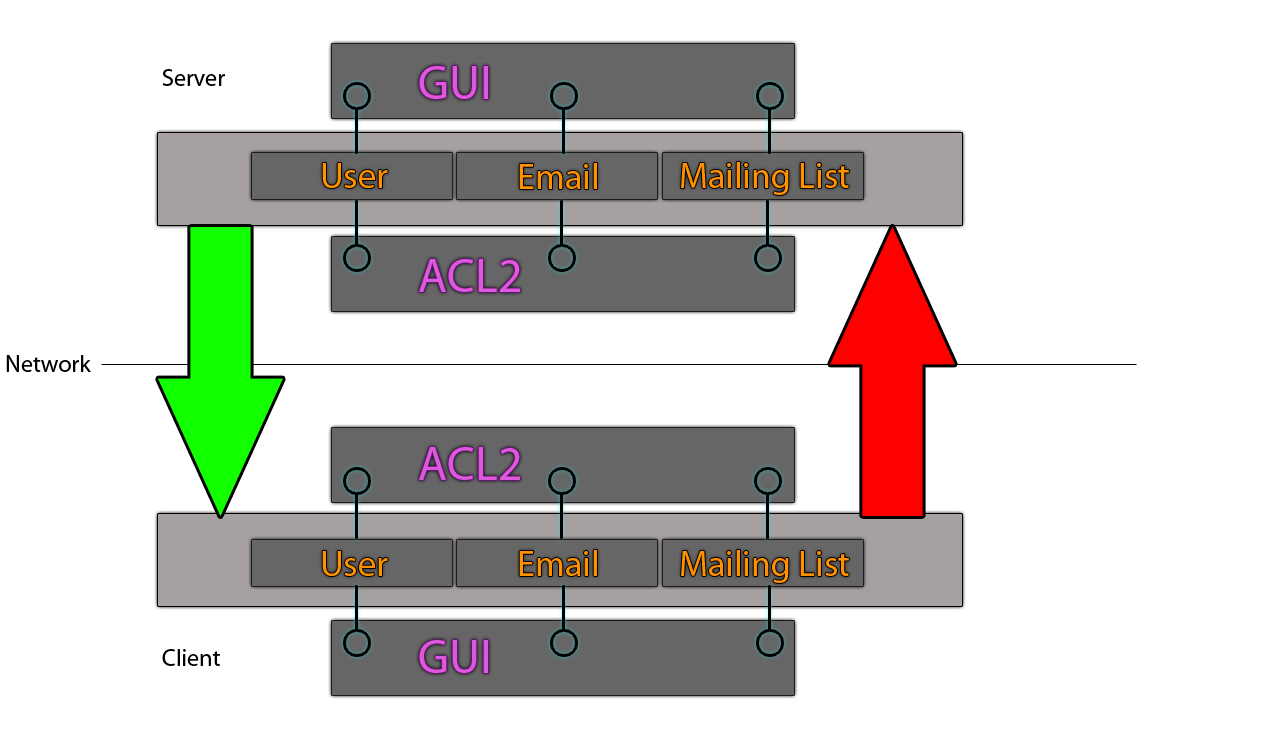
\includegraphics[scale=0.42]{softArch}
\caption{Program Layout}
\end{figure}

There are two separate applications to this program, which must be running in a synchronized fashion.  One is the client, which is the program that invokes the actions upon the program, and the other is the server, which is an automaton after the user starts it on a machine.  This allows the client to send information to the server and expect a response based on the type of transaction it invokes.  Each program consists of a modules, which in itself, is a standalone application.  These modules may be called individually without the GUI intervention.  They are, however, dependent upon ACL2 for data transformation.  The structure of both applications is the same, with a GUI layer for client interaction, an ACL2 layer for data processing and a module layer for integrating the two and providing a means for invocation.

\newpage 
\item[\Large Proof of Concept] \hfill \\ \hfill \\
In order for this project to be feasible, we had to research and test our environments to see if the idea of an email client and server system would be possible. This section will outline our research and tests of the ACL2 and operating system environments. 
\item[ACL2 Environment Research] \hfill \\
Our basis for this project was to develop an application that would implement a network connected application that would have a host program and client programs. Networking is not inherently implemented in ACL2. In order to do this, development of ACL2 modules in Common Lisp would be required. We deemed that this was going to be too much of an undertaking and out of the scope of the Software Engineering - II requirements for the project. \\ \\
In our investigation, we found that the best way to have ACL2 execute from an outside environment is to call the ACL2 system directly from a Java program. Java provides two things that are critical to this application. First, it provides a means of executing ACL2 in a way that eliminates the need for ACL2 executables. Second, it allows us to use local networking protocols to send our message information over a data connection. A Sample of the the Java code that executes this environment follows.

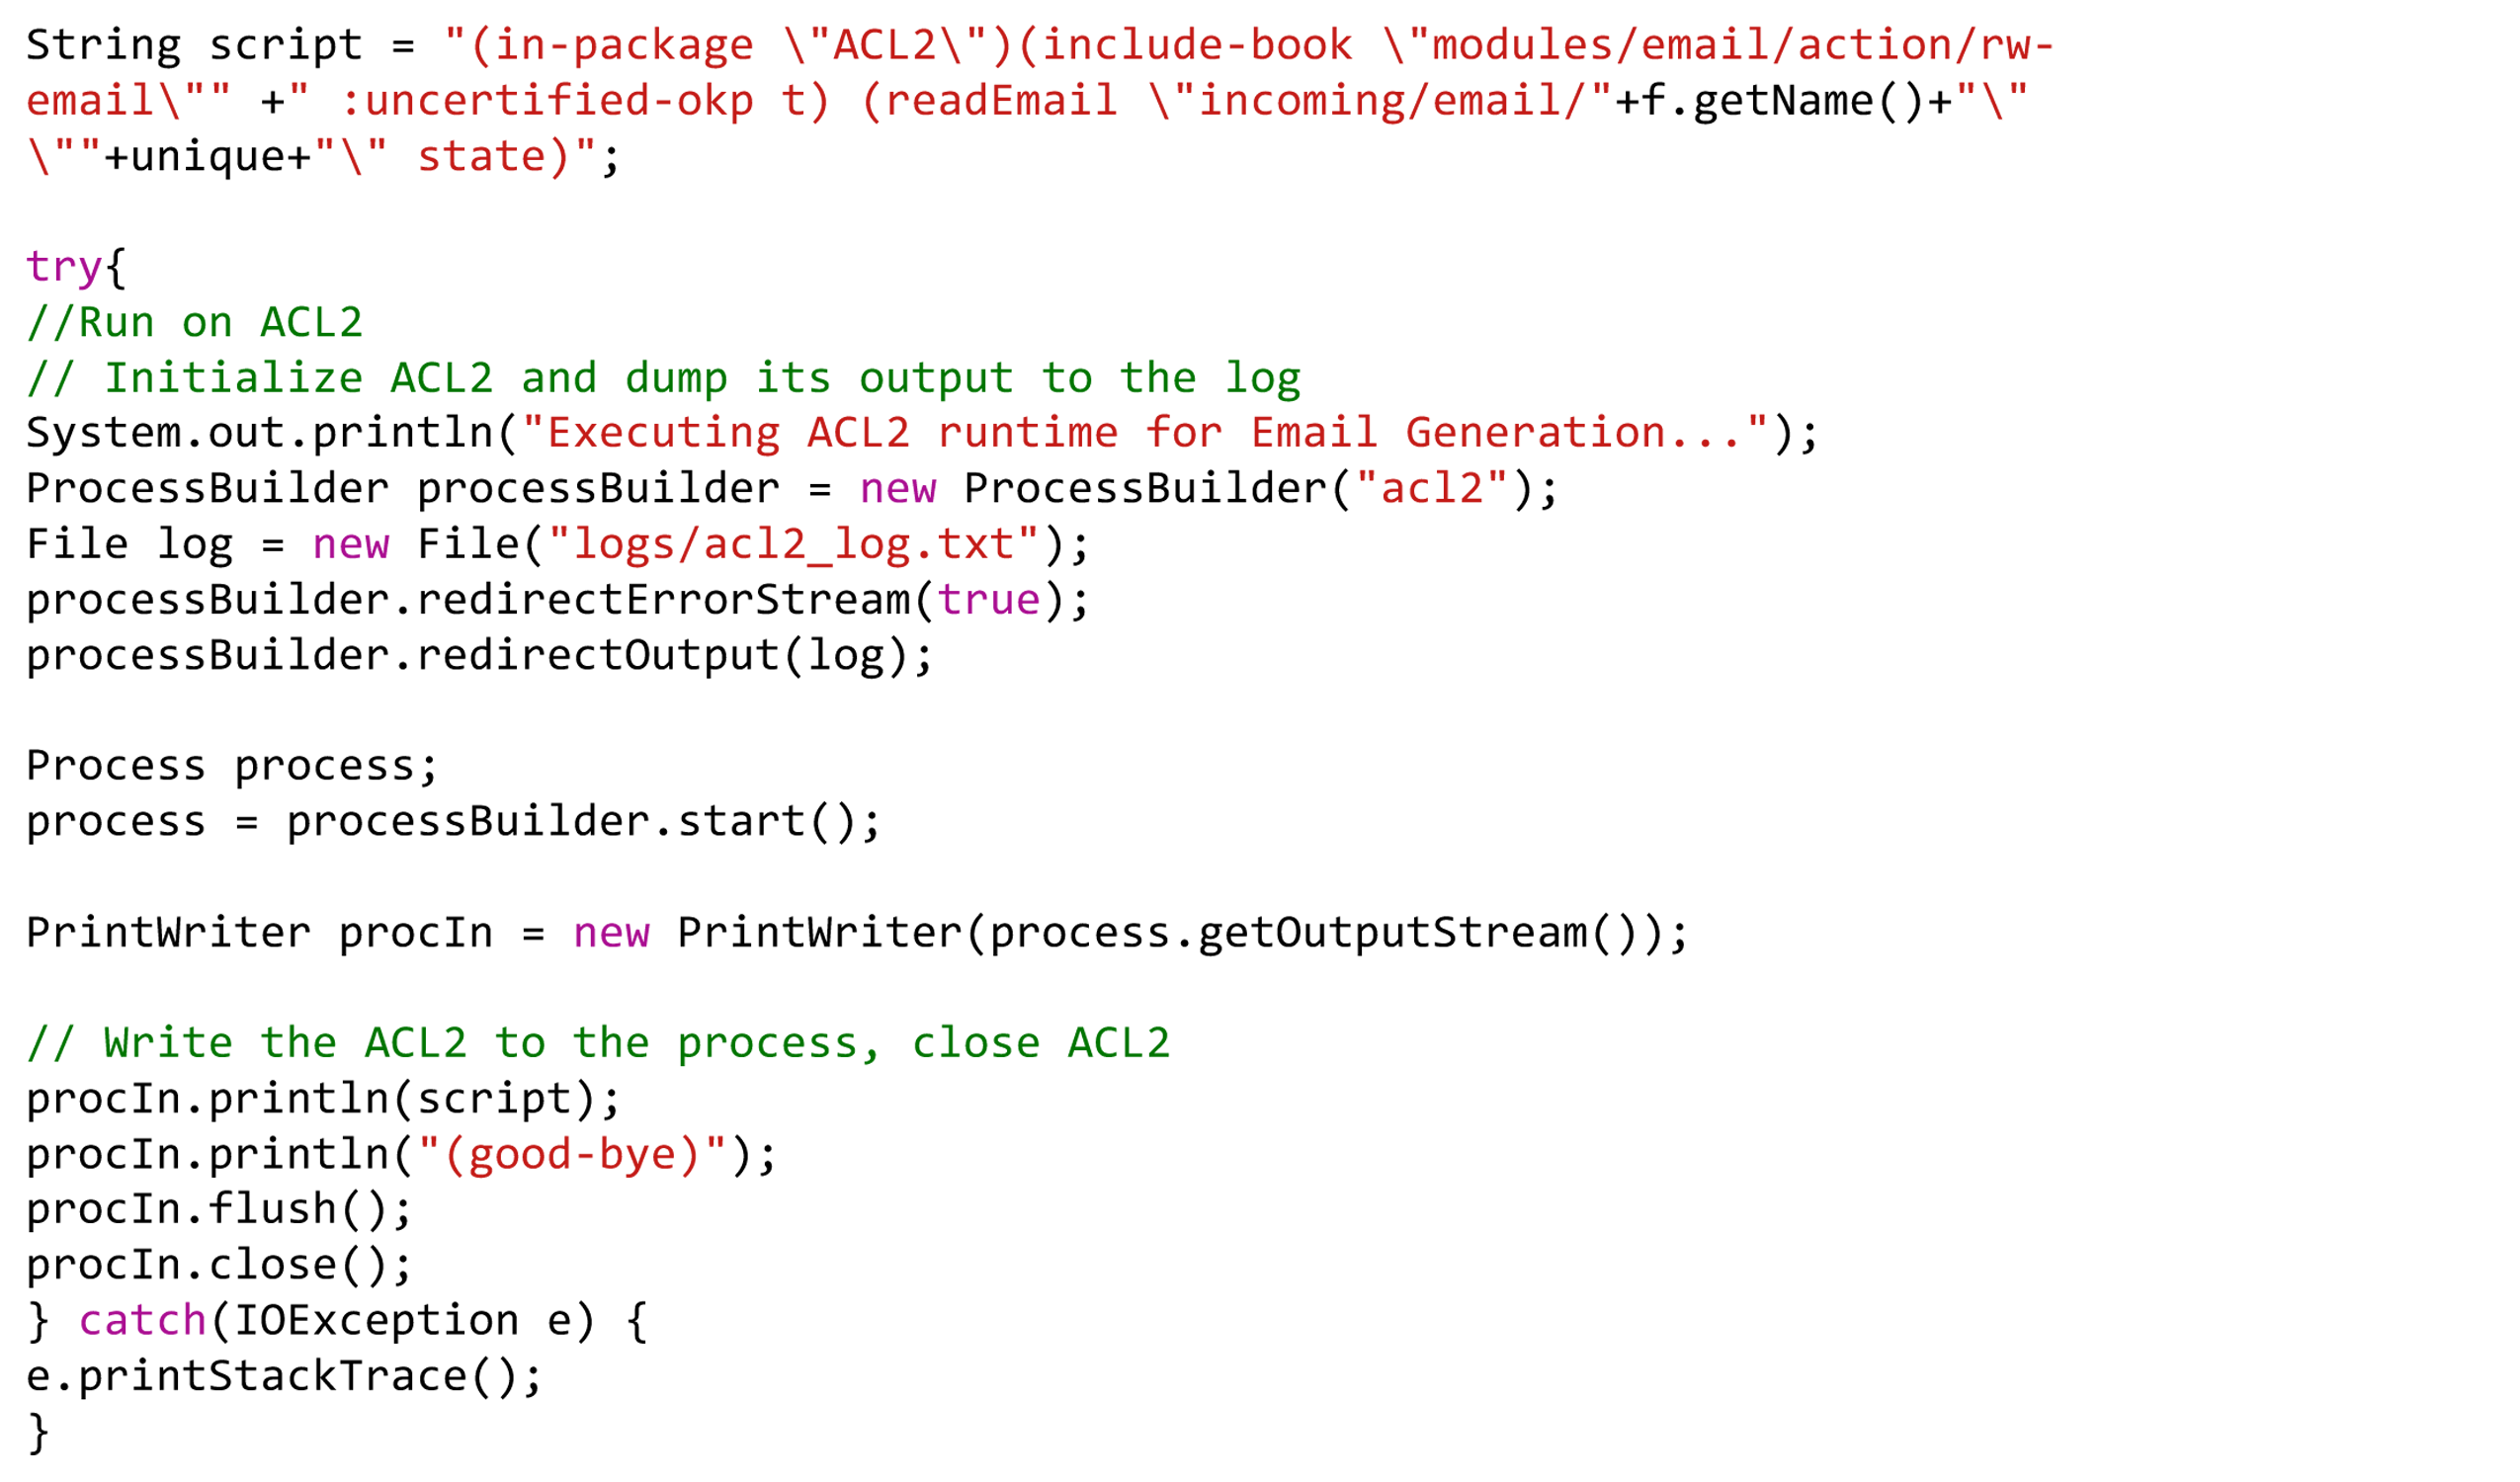
\includegraphics[scale=.8]{javaproc}

Once this process is complete, we can use the built in network modules in Java and have the system send data across a port that is registered with the server.


\newpage
\item[\Large Data Structure Design] \hfill \\ \hfill \\
This project will handle numerous types of data in order to transmit and receive the required information needed for a complete email message. In order to make this process more streamlined and allow effective communications between the different client and server platforms. We have developed the following internal data structures for email messages, address books, contacts, and mailing lists. 
\item[Email Message] \hfill \\
An email message in the scope of this project will contain the following elements. A ``To'' field which will contain the recipient(s) of a message, a ``From'' field to denote the sender of a message, a ``Subject'' field for the message's subject line, and the message field which will hold the content of a message. The ACL2 format of this structure is outlined below: 
\begin{center} $'('(to_1, to_2, ..., to_n) from ``subject" ``message")$\end{center}
Where:\\
$(to_1, to_2, ..., to_n)$: is the recipient email addresses represented as contact structures. \\ \\
$(from)$: is the senders email address in a contact structure. \\  \\
$``subject"$: is the message's subject represented as a string value.\\ \\
$``message"$: is the message's content represented as a string value.

\item[Contact Structure]\hfill \\
Instead of storing email addresses in the format ``name@domain''. We have decided to use a tokenized version of this format which will allow easy access to the contacts information without having to re-parse the address each time we need to find out details of the address. The format of the email address in ACL2 will be: 
\begin{center} $'(domain$ $name)$ \end{center}
Where: \\
$domain$: is the address domain content. This information is the information after the ``@'' symbol in the address. \\ \\
$name$: is the users email name on the domain. This information is written before the ``@'' symbol.

\newpage
\item[Address Registration Structure] \hfill \\ 
In order for a client to send email to another client, it must first register with the server. Server registration will also add a abstracted view of security to the program as well. The registration will take place each time the client is initiated. When initiated, the client will send the server its domain name, user name, and password. This will allow the server to check the registration log and address book to see if the client has registered in the past. If it hasn't, it will add the registration and allow the client to send email messages. \\ \\
The data structure to be used for this process in ACL2 is: 
\begin{center} $'("domain"$ $"name"$  $"password)$\end{center}
Where: \\ 
$domain$: is the address domain content. This information is the information after the ``@'' symbol in the address. \\ \\
$name$: is the user's email name on the domain. This information is written before the ``@'' symbol. \\ \\
$password$: is the user's password used to verify the user with the server and address book and registration log.

\item[Address Book Structure] \hfill \\
The address book will allow a user to search through to view and send email messages to stored contacts. Also this will be used by the server to see if a email address has been registered and is available to receive email messages. The address book will be constructed as: 
\begin{center} $'((``Address String'')_1, (``Address String'')_2, ..., (``Address String'')_n)$ \end{center}
Where: \\
$``Address String''$: is the string value of a registered email client.

\item[Mailing Lists Structure] \hfill \\
A mailing list be used by the clients of the server. This will allow messages to be sent to multiple clients using one address. This will add convenience to the client when sending email messages. The structure of a mailing list will be: 
\begin{center}$ '(``MailingListName''$ $'(contact_1 , contact_2 , ..., contact_n ))$\end{center}
Where:\\
$``MailingListName''$: is the string value of the mailing list's name. \\ \\
$contact_n$: is a contact in the mailing list. This will be stored as a contact structure as defined above.


\newpage
\item[\Large Component Requirements] \hfill \\ \hfill \\
The program is split into two separate programs. The server program will handled the communications between the clients. The client program will handle all user end features and input. Each program is built in a modular fashion and the detailed structure of each module will be discussed in the next section. 
\item[\large Server]\hfill \\
The server will need the following modules for implementation. The requirements for each module are: 
\item[Email]\hfill \\
This is one of the most important modules as it will handle the message interaction between the client and server. The server will need to implement the following in order to successfully handle email messages.
\begin{itemize}
\item Open an email message from a file in XML format and save the message in a client's inbox in XML format.
\item Split an incoming message into it individual components.
\item Read email addresses and generate store directories for saving XML files.
\item Parse an incoming email into XML tokens
\item Monitor port 20005 for incoming messages. Then save incoming messages into the incoming email directory
\end{itemize}
\item[User]\hfill \\
The User module will need to accomplish two task. The first task will be to register new users into the system. Once a user has been registered, the client will have an inbox available on the server. The next task will be to verify a user and send the user its email messages. The specific task for this module are:
\begin{itemize}
\item Create and maintain an email address book of active users.
\item Take a user request and generate an email address entry into the address book.
\item Assign a password to a user.
\item Check to see if a user is already entered into the address book.
\item Verify a users password
\item Verify a user request as belonging to the user
\item Upon verification send all email messages on server to the user.
\item Monitor the network on port 20003 for user registration request
\item Monitor the network on port 20002 for verification request
\end{itemize}
\newpage
\item[Mailing List]\hfill \\
The mailing list will be a feature that will allow a user to send a message to multiple recipients by sending an email to an alias address that is registered on the server. Users must have permission to send messages to a mailing list and must be able to request access to either send and receive messages from a mailing list. Specifically the mailing list should:
\begin{itemize}
\item Allow a user to request a mailing list be created.
\item Allow a user to request access to the mailing list
\item Allow a user to request to be removed from the list.
\item Recognize the email alias as a mailing list address.
\item Upon list recognition, copy the email and send to users on the list.
\end{itemize}

\item[\large Client]\hfill \\
The client program will be the point of interaction for the users of the system. The client will need these modules in order to interact with the server.
\item[Email]\hfill \\
The client email module will need to be able to read and write messages to or from the server. The functionality needed for the email module is:
\begin{itemize}
\item Allow a user to input an email message to send to another client.
\item Generate the correct XML format from the inputted email message.
\item Allow a user to send a single message to multiple recipients.
\item Split a multiple recipient email message into separate XML documents for each message.
\item Process an incoming email in XML format and convert the email to HTML for the client's inbox.
\item Connect to the server over port 20005 and send an email XML file to the server for processing
\item Connect to the server over port 20002 and retrieve email messages waiting for the client on the server. 
\end{itemize}
\item[User]\hfill \\
The user module on the client will be used to register the client on the server. The User module will need to:
\begin{itemize}
\item accept as input the username, domain, and password of a client.
\item Generate a request XML file with the given information for the request.
\item Connect to the server on port 20003 to send the request file.
\end{itemize}
\item[Mailing List]\hfill \\
The mailing list will allow a client to send messages to multiple clients with one alias. The mailing list will need to:
\begin{itemize}
\item Accept as input, the name and recipients for the mailing list.
\item Generate a new mailing list request XML file to send to the server.
\item Generate a request file to be added to a mailing list.
\item Generate a request file to be removed from a mailing list.
\item Generate a request to obtain access to a mailing list.
\end{itemize}

\newpage
\hypertarget{Component Design} {}
\item[\Large Module Design] \hfill \\ \hfill \\
There are two separate applications to this program. Both must be running in some synchronized fashion. The first being the client, which is the program that will invoke actions on the user end of the application and make request to the server. Then the server, which is an automaton, will process request and send appropriate information back to the clients. Each program will consist of modules specific to the operation of the program. This section will discuss the exact structure for modules on both the client and server since each application has subtle differences in its development. \\
\item[\large Server Design] \hfill \\ \hfill \\
This section will cover the design standards of the server program and general module structure. The server is divided into three parts: An ACL2 module, the actions the module performs, and a GUI interface for easy startup and shutdown processes.
\item[ACL2]\hfill \\
The structure of the ACL2 that is implemented on the program consists of 3 separate parts:\\
1.	The Logic\\
2.	The Tests\\
3.	The Actions\\\\
\textit{The Logic}\\\\
The logic consists of the transformations that will occur upon the proposed data structures in the application.  An example of this would be the address-book.lisp file.\\

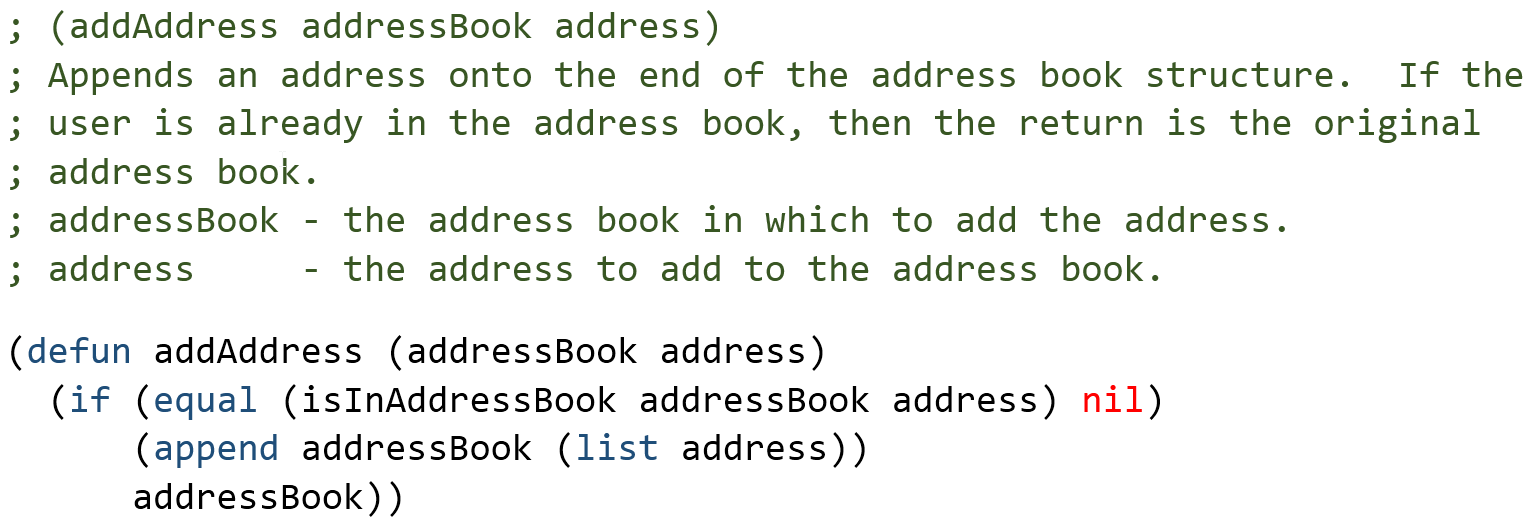
\includegraphics[scale=.3]{addbk}\\

In this code snippet, we examine the addressBook, which is a user defined structure – a list of addresses, address containing a domain, name and password.  It uses a user defined function in order to determine whether the address is in the addressBook structure and if that is false, then we can append the address to the list of addresses.  If not, then it is already in the addressBook, thus we can return the original addressBook.  \\\\
There is not technically a type enforcement on this data, as it can actually hold numerical values.  We can safely assume that we are not concerned with the type value until actionable information is passed from the invocation portion of the script – since we can explicitly cast this information, but safely assume our testing can include any such value this logic can be tested again – including integers, null values, strings, and even lists of strings.  It suffices to say, at the logic level, we are not considerably concerned with the data the user has entered, rather whether the transformations are correct and true.  This absolves the developer from considering this issue and allows them to focus explicitly on the logic.\\\\
The logic should be included in the modules root folder and a name given (such as users in the case of the example: \textit{modules/users/address-book.lisp}).  We will go into actions a bit later, but it is safe to say that anything that invokes this file should be a part of this module. \\ \\
\textit{The Test} \\ \\
Testing is done via Racket utilizing the Dracula environment.  There are three alternative methods of testing – two of which are discrete, and one through induction.  Proof through induction is the most solid means of verifying the transformations from the logic are true and correct.  The other two include property based randomized testing (PBRT), and check-expects.\\\\

Proof through induction must be implemented through the ACL2 engine.  You can use Racket in order to prove the formulated hypothesis, thus accepting it as a theorem into the logical world.\\

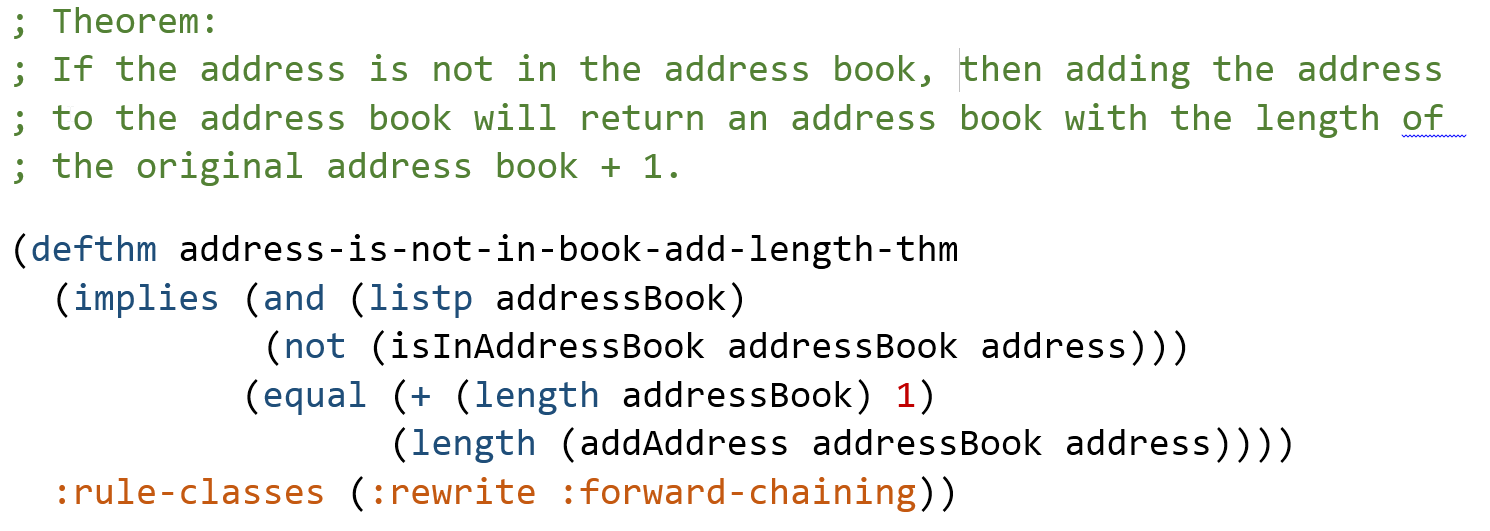
\includegraphics[scale=.3]{svrthm}\\

In this example, we are verifying that if we add an address to the addressBook structure that is currently not a part of the addressBook, we can conclude that the size of the addressBook is increased by one.  Using the theorem prover yields us our result:
\scriptsize{\begin{verbatim}
ACL2 Observation in ( DEFTHM ADDRESS-IS-NOT-IN-BOOK-ADD-LENGTH-THM...):  The :TRIGGER-TERMS for the :FORWARD-CHAINING 
rule 
ADDRESS-IS-NOT-IN-BOOK-ADD-LENGTH-THM will consist of the list containing (LISTP ADDRESSBOOK).
ACL2 Warning [Non-rec] in ( DEFTHM ADDRESS-IS-NOT-IN-BOOK-ADD-LENGTH-THM...):  A :REWRITE rule generated from 
ADDRESS-IS-NOT-IN-BOOK-ADD-LENGTH-THM will be triggered only by terms containing the non-recursive
 function symbol LENGTH.  Unless this function is disabled, this rule is unlikely ever to be used.
ACL2 Warning [Free] in ( DEFTHM ADDRESS-IS-NOT-IN-BOOK-ADD-LENGTH-THM...):  A :REWRITE rule generated
 from ADDRESS-IS-NOT-IN-BOOK-ADD-LENGTH-THM contains the free variable ADDRESS.  This variable will be
  chosen by searching for an instance of (NOT (ISINADDRESSBOOK ADDRESSBOOK ADDRESS)) in the context of
  the term being rewritten.  This is generally a severe restriction on the applicability of a :REWRITE
   rule.  See :DOC free-variables.
ACL2 Warning [Subsume] in ( DEFTHM ADDRESS-IS-NOT-IN-BOOK-ADD-LENGTH-THM...):  The previously added
 rule COMMUTATIVITY-OF-+ subsumes a newly proposed :REWRITE rule generated from
  ADDRESS-IS-NOT-IN-BOOK-ADD-LENGTH-THM, in the sense that the old rule rewrites a more general
   target.  Because the new rule will be tried first, it may nonetheless find application.
ACL2 Warning [Free] in ( DEFTHM ADDRESS-IS-NOT-IN-BOOK-ADD-LENGTH-THM...):  
When the :FORWARD-CHAINING rule generated from
ADDRESS-IS-NOT-IN-BOOK-ADD-LENGTH-THM is triggered by (LISTP ADDRESSBOOK) it contains the free
 variable ADDRESS.  This variable will be chosen by searching for an instance of (NOT (ISINADDRESSBOOK
  ADDRESSBOOK ADDRESS)) among the hypotheses of the conjecture being rewritten.  This is generally a
   severe restriction on the applicability of the forward chaining rule.
ACL2 Warning [Non-rec] in ( DEFTHM ADDRESS-IS-NOT-IN-BOOK-ADD-LENGTH-THM...):  The term (LISTP
 ADDRESSBOOK) contains the non-recursive function symbol LISTP.  Unless this function is disabled,
  (LISTP ADDRESSBOOK) is unlikely ever to occur as a trigger for ADDRESS-IS-NOT-IN-BOOK-ADD-LENGTH-THM.
<< Starting proof tree logging >>
Goal'
([ A key checkpoint:
Goal'
(IMPLIES (AND (CONSP ADDRESSBOOK)
              (NOT (ISINADDRESSBOOK ADDRESSBOOK ADDRESS)))
         (EQUAL (+ 1 (LEN ADDRESSBOOK))
                (LEN (APPEND ADDRESSBOOK (LIST ADDRESS)))))
*1 (Goal') is pushed for proof by induction.
])
Perhaps we can prove *1 by induction.  Three induction schemes are suggested by this conjecture. 
 Subsumption reduces that number to two. These merge into one derived induction scheme.  We will
  induct according to a scheme suggested by (LEN ADDRESSBOOK), but modified to accommodate
   (ISINADDRESSBOOK ADDRESSBOOK ADDRESS).
These suggestions were produced using the :induction rules BINARY-APPEND, ISINADDRESSBOOK and LEN.  If
 we let (:P ADDRESS ADDRESSBOOK) denote *1 above then the induction scheme we'll use is
(AND (IMPLIES (NOT (CONSP ADDRESSBOOK))
              (:P ADDRESS ADDRESSBOOK))
     (IMPLIES (AND (CONSP ADDRESSBOOK)
                   (:P ADDRESS (CDR ADDRESSBOOK)))
              (:P ADDRESS ADDRESSBOOK))).
This induction is justified by the same argument used to admit LEN.  When applied to the goal at hand
 the above induction scheme produces three nontautological subgoals.
Subgoal *1/3
Subgoal *1/2
Subgoal *1/1
Subgoal *1/1.2
Subgoal *1/1.1
*1 is COMPLETED!
Thus key checkpoint Goal' is COMPLETED!
Q.E.D.
Summary
Form:  ( DEFTHM ADDRESS-IS-NOT-IN-BOOK-ADD-LENGTH-THM ...)
Rules: ((:DEFINITION ADDADDRESS)
        (:DEFINITION BINARY-APPEND)
        (:DEFINITION ISINADDRESSBOOK)
        (:DEFINITION LEN)
        (:DEFINITION LENGTH)
        (:DEFINITION LISTP)
        (:DEFINITION NOT)
        (:EXECUTABLE-COUNTERPART BINARY-+)
        (:EXECUTABLE-COUNTERPART CONSP)
        (:EXECUTABLE-COUNTERPART EQUAL)
        (:EXECUTABLE-COUNTERPART LEN)
        (:EXECUTABLE-COUNTERPART LENGTH)
        (:FAKE-RUNE-FOR-TYPE-SET NIL)
        (:INDUCTION BINARY-APPEND)
        (:INDUCTION ISINADDRESSBOOK)
        (:INDUCTION LEN)
        (:REWRITE CDR-CONS)
        (:REWRITE COMMUTATIVITY-OF-+)
        (:TYPE-PRESCRIPTION BINARY-APPEND)
        (:TYPE-PRESCRIPTION ISINADDRESSBOOK)
        (:TYPE-PRESCRIPTION TRUE-LISTP-APPEND))
Warnings:  Subsume, Free and Non-rec
Time:  0.00 seconds (prove: 0.00, print: 0.00, proof tree: 0.00, other: 0.00)
Prover steps counted:  1017
 ADDRESS-IS-NOT-IN-BOOK-ADD-LENGTH-THM
\end{verbatim}}
\normalsize
As we can see, the theorem has been accepted and the inductions require are listed above.  It also goes into a full textual description of the proving steps and lists the number of steps required to prove the function.  Thus we can assume that the logic for adding an address to the addressBook is theoretically sound.\\\\
PBRT describes a hypothesis of the transformation of a function to be tested.  Random values are assigned, and injected into this logic and tested for its trueness.  The range of testing can be user specified, but for our sake, we have implemented a default value of 50 cycles.  The formulation of the proof structure is similar to that of the theorem test, but we are required to define out input values.
\\\\
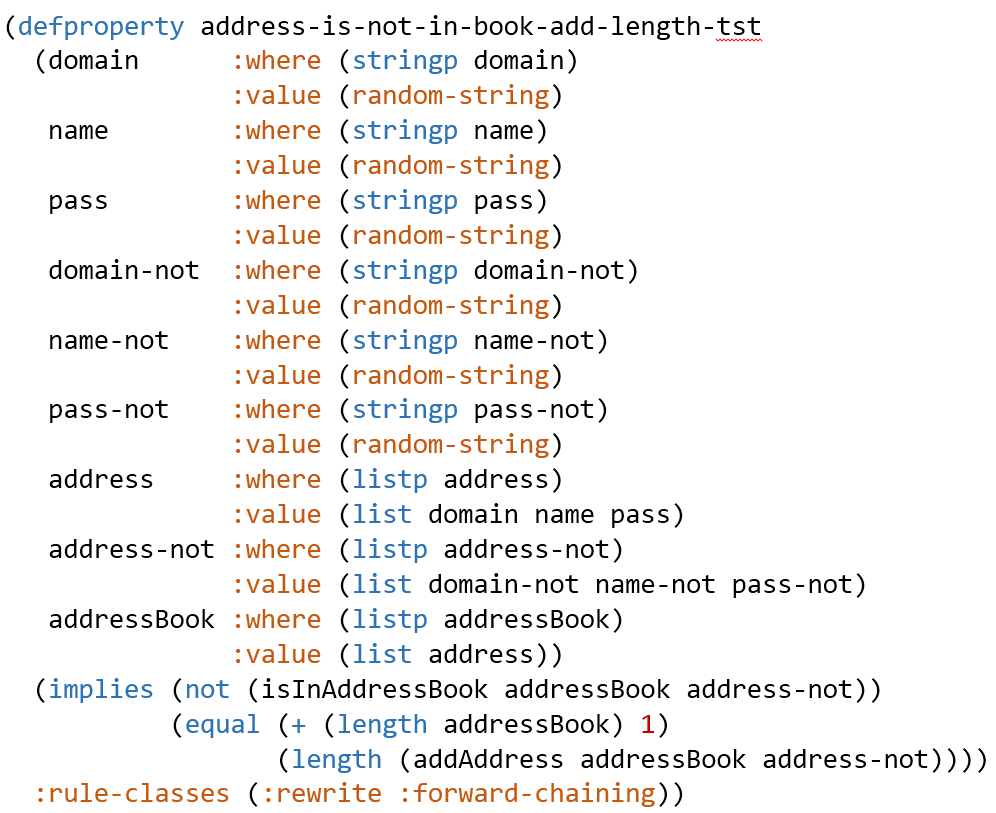
\includegraphics[scale=.4]{pbrt}\\\\ 
%\newpage
We are using exactly the same hypothesis that we proved in ACL2.  The only different is the discrete values that are populated.  Though these values are considered to be random, they are limited, this is not a correct bearing for the correctness of the hypothesis, but rather standard foundation for augmenting out hypothesis if we are unable to get it to verify correctly in ACL2.  The results of this test are: 
\begin{center}
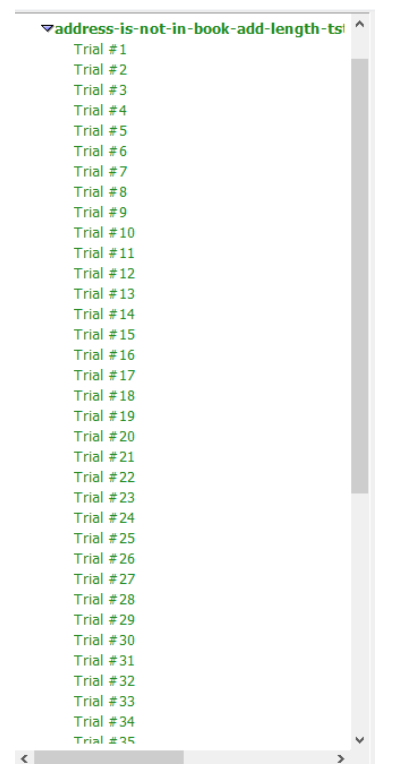
\includegraphics[scale=0.3]{rst}
\end{center}
We can view each individual trial, thus if there is an error, we can see the values as opposed to trying to change our hypothesis based on theoretical results – usually it is more intuitive for developers to see a value that is causing it to fail.\\ \\
Sometimes developers may find this process frustrating as theory is generally more difficult to prove over that of expected results with known inputs.  This is where the check-expect typically helps.  With it, we can enter a value that we predetermine and verify it against the expected output (producing a true/false result).\\\\
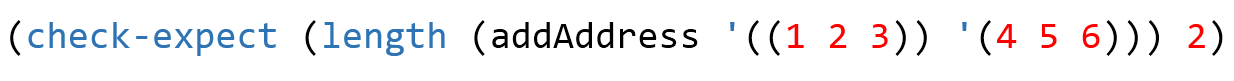
\includegraphics[scale=0.3]{chkex}\\\\
This statement states  that if we add the address \textit{(4 5 6)} to the addressBook that contains \textit{(1 2 3)} only, we will acquire the addressBook with the additional address, verified by the length of the total address book – in this case, addressBook is a list of lists or numbers (three values).  Running this test will only result in an echo of ``test passed'' or ``test failed'', with no reasoning.\\\\
Typically these logic files are included in the modular folder with the logic file (usually suffixed by \_tests).  No naming conventions are enforced at this level other than knowing that this file is not to be invoked by the ACL2 subsystem when the module is running.  It is explicitly used for testing purpose.
\\\\
\textit{The Actions}\\\\
Logic is for naught if we are not doing anything with it.  This is where our actions come into play and the integration into or client/server environment.  The actions are the standalone program portion of the module that that will perform the IO as well as any network connectivity.  Portions of this are written in ACL2 and others are written in Java.  There were some considerations previously of writing the whole module in ACL2, but network connectivity proved to be a challenge.  This was later changed to shell scripting in the BASH shell, but synchronization through connectivity, yet again, proved to be an issue.  We could send information across a network, but waiting for a response proved to be an issue.  In the end, we decided that Java was the best alternative and many students would integrate into this environment seamlessly.  This is also where the client and server start to deviate in code production.\\

\item[The Module]\hfill \\
There are typically two parts to the action of each module, but a user can define as many as they need to complete the task.  You can implement GUI elements in this application or you may even perform some third party processing to get the information ready for ACL2 processing.  For the sake of demonstration, we will be implementing this in a simplistic manner through the user registration process.\\\\
Since the action we defined is register, a subfolder in the \textit{user} folder is created and will contain the files responsible for registration.  We can define the files as needed, but we are going to invoke against the RegisterUser class.  Since the execution of the server occurs from the root, we must include this Java class in the package: ``\textit{modules.user.register}'' which makes the fully qualified name for invocation \textit{modules.user.register.RegisterUser}.  More will be compounded upon this when the GUI wrapper is introduced.  We also need a minimum of one lisp file that will generate IO for the ACL2 environment and put the logic to work on data structures.  This is also the point to which the user should be concerned with the data types being introduced into the ACL2 environment, since it will be responsible for writing persistent data.\\\\
Example of lisp required:\\
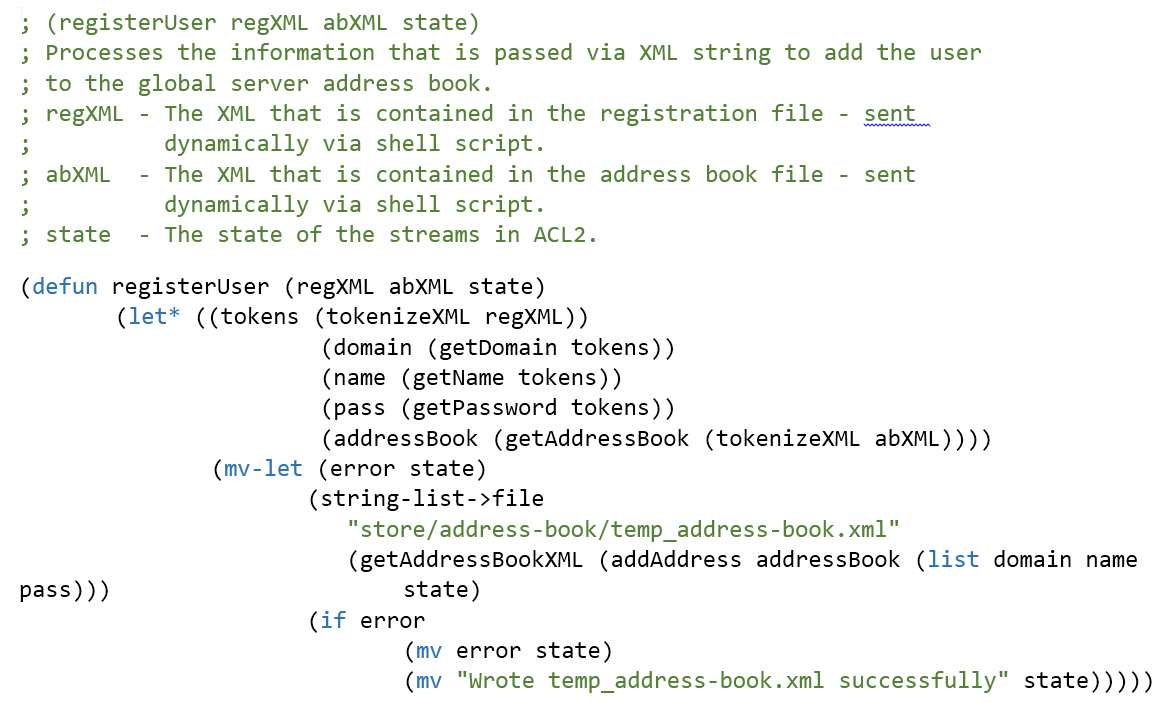
\includegraphics[scale=0.5]{lisp}\\\\
This example provides an entry point that will attempt to add the user to the addressBook and store it for persistence.  There are a couple of things to note – we are writing to \textit{temp\_address-book.xml} which generally does not denote permanent storage, but because of one of the shortcomings of ACL2, we cannot overwrite a file that is currently open for read.  This will be expanded upon when we discuss the GUI integration. \\

The XML is tokenized from the incoming request, parsed into the address and addressBook data structures.  This information is fed directly from the Java file into this function and pushed into ACL2.  The response is written and additional logic in the Java file ensures that the addressBook data structure has changed by verifying the sizes of the \textit{temp\_address-book.xml} and \textit{address-book.xml} files.
We can then move on to the java file construction.  In this file, the networking (if needed) and typical IO functions that cannot be handled by ACL2 generally occur.  Since this is a standalone application, it must have a main method associated in the file.  From there we can call the \textit{ProcessBuilder}, and invoke ACL2 by building ``wrappers'' for the ACL2 input and output.  You are able to feed ACL2 commands and functions directly into the environment, after which you must call (good-bye) in order to exit the process.  General cleanup of memory must occur and the process is repeated for every incoming request.\\

After the Java file is constructed, you must compile it and register the binary in the server module registration manager (for server side modules).  Client side requires integration into the application at this point, which is direct manipulation of the source code and recompilation.\\
\item[The GUI]\hfill \\
Modules are invoked from a \textit{ProcessBuilder} similar to the one that invokes ACL2.  This requires that we register each module so the user can identify it.  Since this is allowed on the server side, there is no overhead for integration into the Server UI, rather just standalone application specifics that are introduced when the module has been ran.\\\\
To register the module on the server, execute the Server class through a console (java Server).  A GUI should show up with a menu at the top of the screen.  Under the ``modules'' menu, you will find ``management''.  Clicking this will open a list of modules currently registered with the server and by clicking the ``add'' button, you can add the module.  It is important to note that you cannot register modules that are listening on the same network port.  They will create a confliction and fail to start.  The registration will simply reject it completely.  The fields are fairly straight forward with the name of the module, location and port.  Location can be selected via the locator button, which will generate the expected package name for invocation.

\item[\large Client Design]\hfill \\ \hfill \\
The client is developed into modules with three major components: the logic, test, and actions. Each module runs independently from each other, thus making each module a stand alone application itself. The modules are tied together into the GUI in order to make reading the results and executing the application easier. However, the GUI is not needed in order to make the application run. The layout of each layer is described below. \\
\item[ACL2]\hfill \\
The ACL2 components are structured into 3 parts:
1.	The Logic
2.	The Test
3.	The Actions \\ \\
\textit{Logic}\\
The logic consists of transformations that need to be handled by the proposed data structures in the application. An example of this would be the client-email.lisp file.\\\\
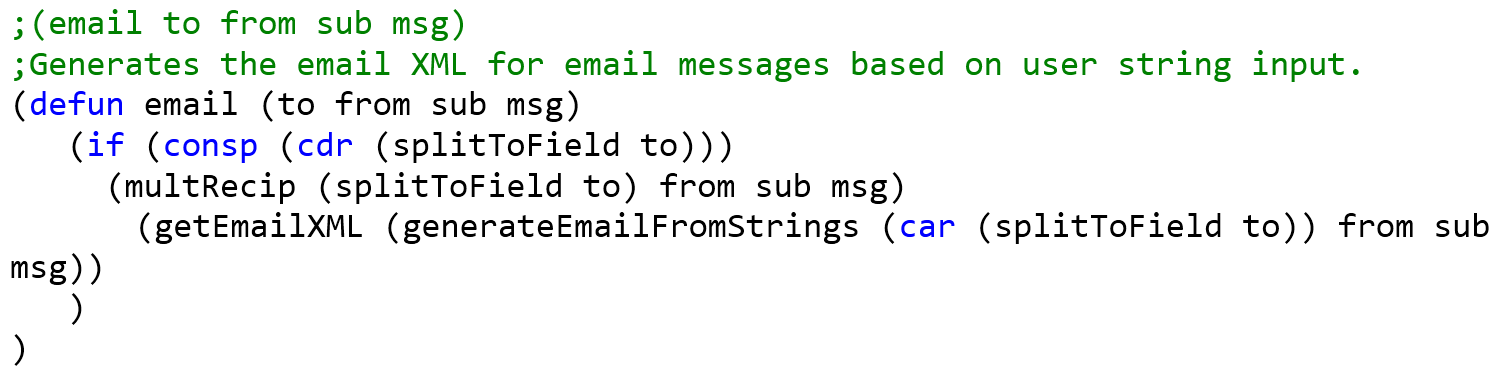
\includegraphics[scale=0.3]{clientlisp}\\\\
In this code, we take in the contents of an email message that will need to be generated into an XML format. The function takes in four parameters with each being a corresponding component to an email message. Once the function has completed, we are left with the XML contents for an email message that will then need to be stored for output, which will be handled in the actions component. An example of the raw XML output would be:
\begin{verbatim}
<?xml version='1.0'?><!DOCTYPE user SYSTEM '../../../dtd/messages.dtd'>
<email>
    <to>howell@localHost</to>
    <from>crist@localhost</from>
    <subject>SUB001</subject>
    <content>MSG001</content>
</email>
\end{verbatim}
As you can see, each of the four fields is generated into an email message format. This XML format is strictly defined in the document type definition located in the directory specified. This DTD must be included on BOTH the client and server in order for the XML definitions to pass.

Logic files will need to be stored in the root directory of the module and given a name such that it represents the logic it is performing (For the above example, the email module on the client is stored in the following directory: modules/email/client-email.lisp). Any operation that needs to include this main logic file should be part of this module.\\\\
\textit{Test}\\\\
Testing is done through the Dr. Racket and Dracula interface. There are three methods of testing which include Theorems, Properties, and Checks. Theorems are proofs through induction of your methods. Properties and Checks utilized specified and random data to test your code for expected outputs. 

Proofs through inductions that are accomplished through the theorems are the soundest way of testing your logic code. It is safe to say that if your theorem passes your inductive hypothesis, your function produces correct output according to your hypothesis.  You can use Dr. Racket for theorem proving. An example theorem would be:\\\\
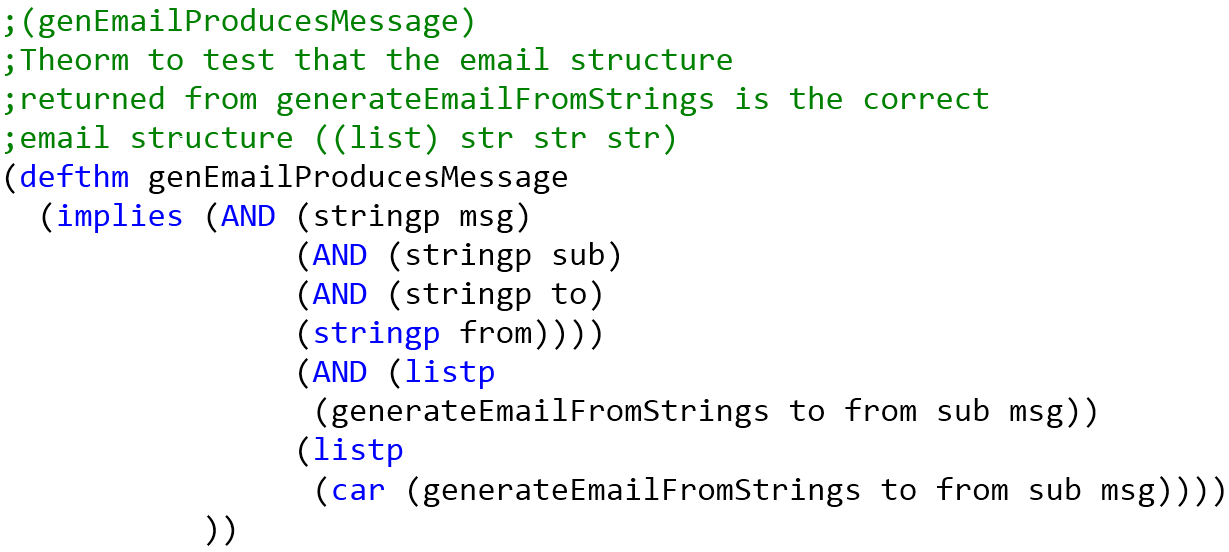
\includegraphics[scale=0.35]{clienttest}\\\\
This theorem proves that an email message structure is returned from the generateEmailFromStrings function. It test to see if the format of the output follows this format. \verb$((list) str str str)$ If it does, then the correct structure of an email message has been processed and returns a true result. Since this theorem passes ALC2 logic, it is safe to say that our logic produces the desired output.\\ 

Property based testing and Check Expects are needed to test boundary cases of your logic functions. These forms of testing are useful if you are experiencing trouble with specified conditions and if random data is needed for your project. Since the email client relies heavily on invariant data, these forms of testing are not idea for this application.\\

It is also worth noting that through the Racket interface, a property-based test can be passed to the ACL2 logic mechanism. The same logical induction is performed on the properties and its results are the same as if the test were a theorem. So you can use a property as if it were a theorem in this case.\\

\textit{Actions}\\\\
The actions are where the logic portions of the module are executed. The actions file should contain all the external dependencies of the module. Also the actions should also perform all the IO operations for your logic. This is done to help the module become its own stand alone application. In the client, the actions layer is developed into two programs. A Java program handles the invocation and network connections, and the ACL2 program which handles the ALC2 logic and IO for the module. \\

We need to expand on the Java program. Each module will need a Java program to be included with the actions of a module. This will take care the network connections, ACL2 invocation, and interfacing with the GUI. The Java program will need to be developed as a library, which deviates from the server. This will allow the module to stand on its own, as well as be expanded on in the future.  An example of a header for the Java program follows:\\\\
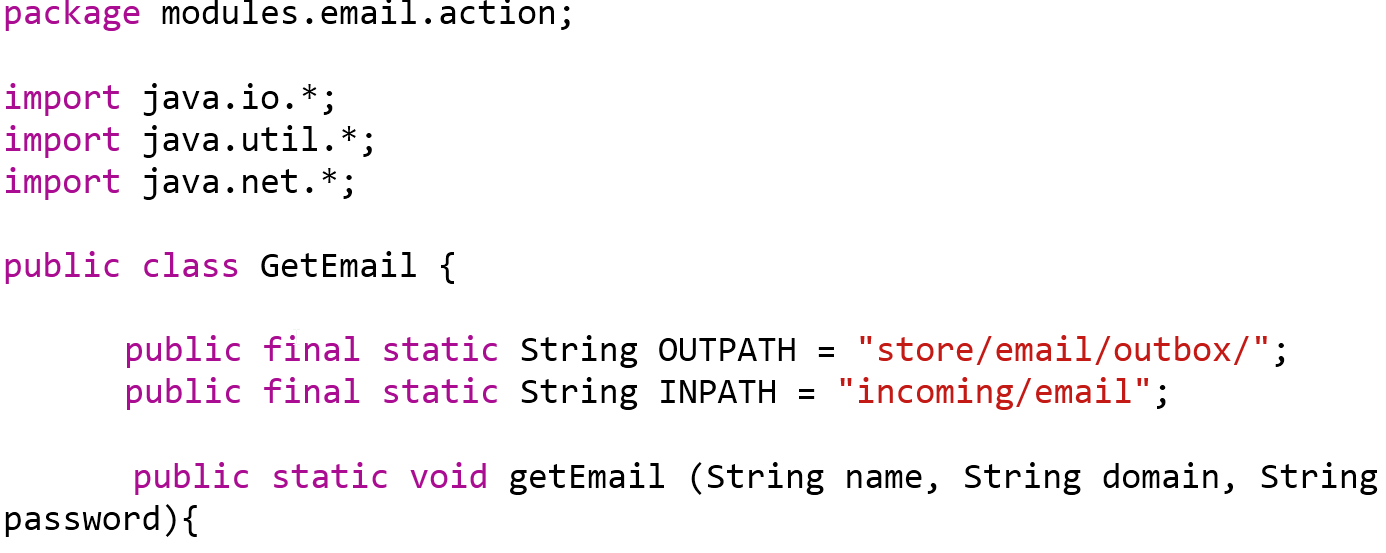
\includegraphics[scale=0.35]{javapkg}\\\\
As you can see, this Java program is registered in a package. This package will need to match your file path the location of your Java class. This will allow other applications in the client program to import your Java class and use its functions. \\

Also this program will contain statically defined functions, which the calling program will be able to use. These functions will use Java’s ProcessBuilder to build out a process to ACL2 and run the ACL2 environment. An example of the ACL2 call for this action is on the following page:\newpage
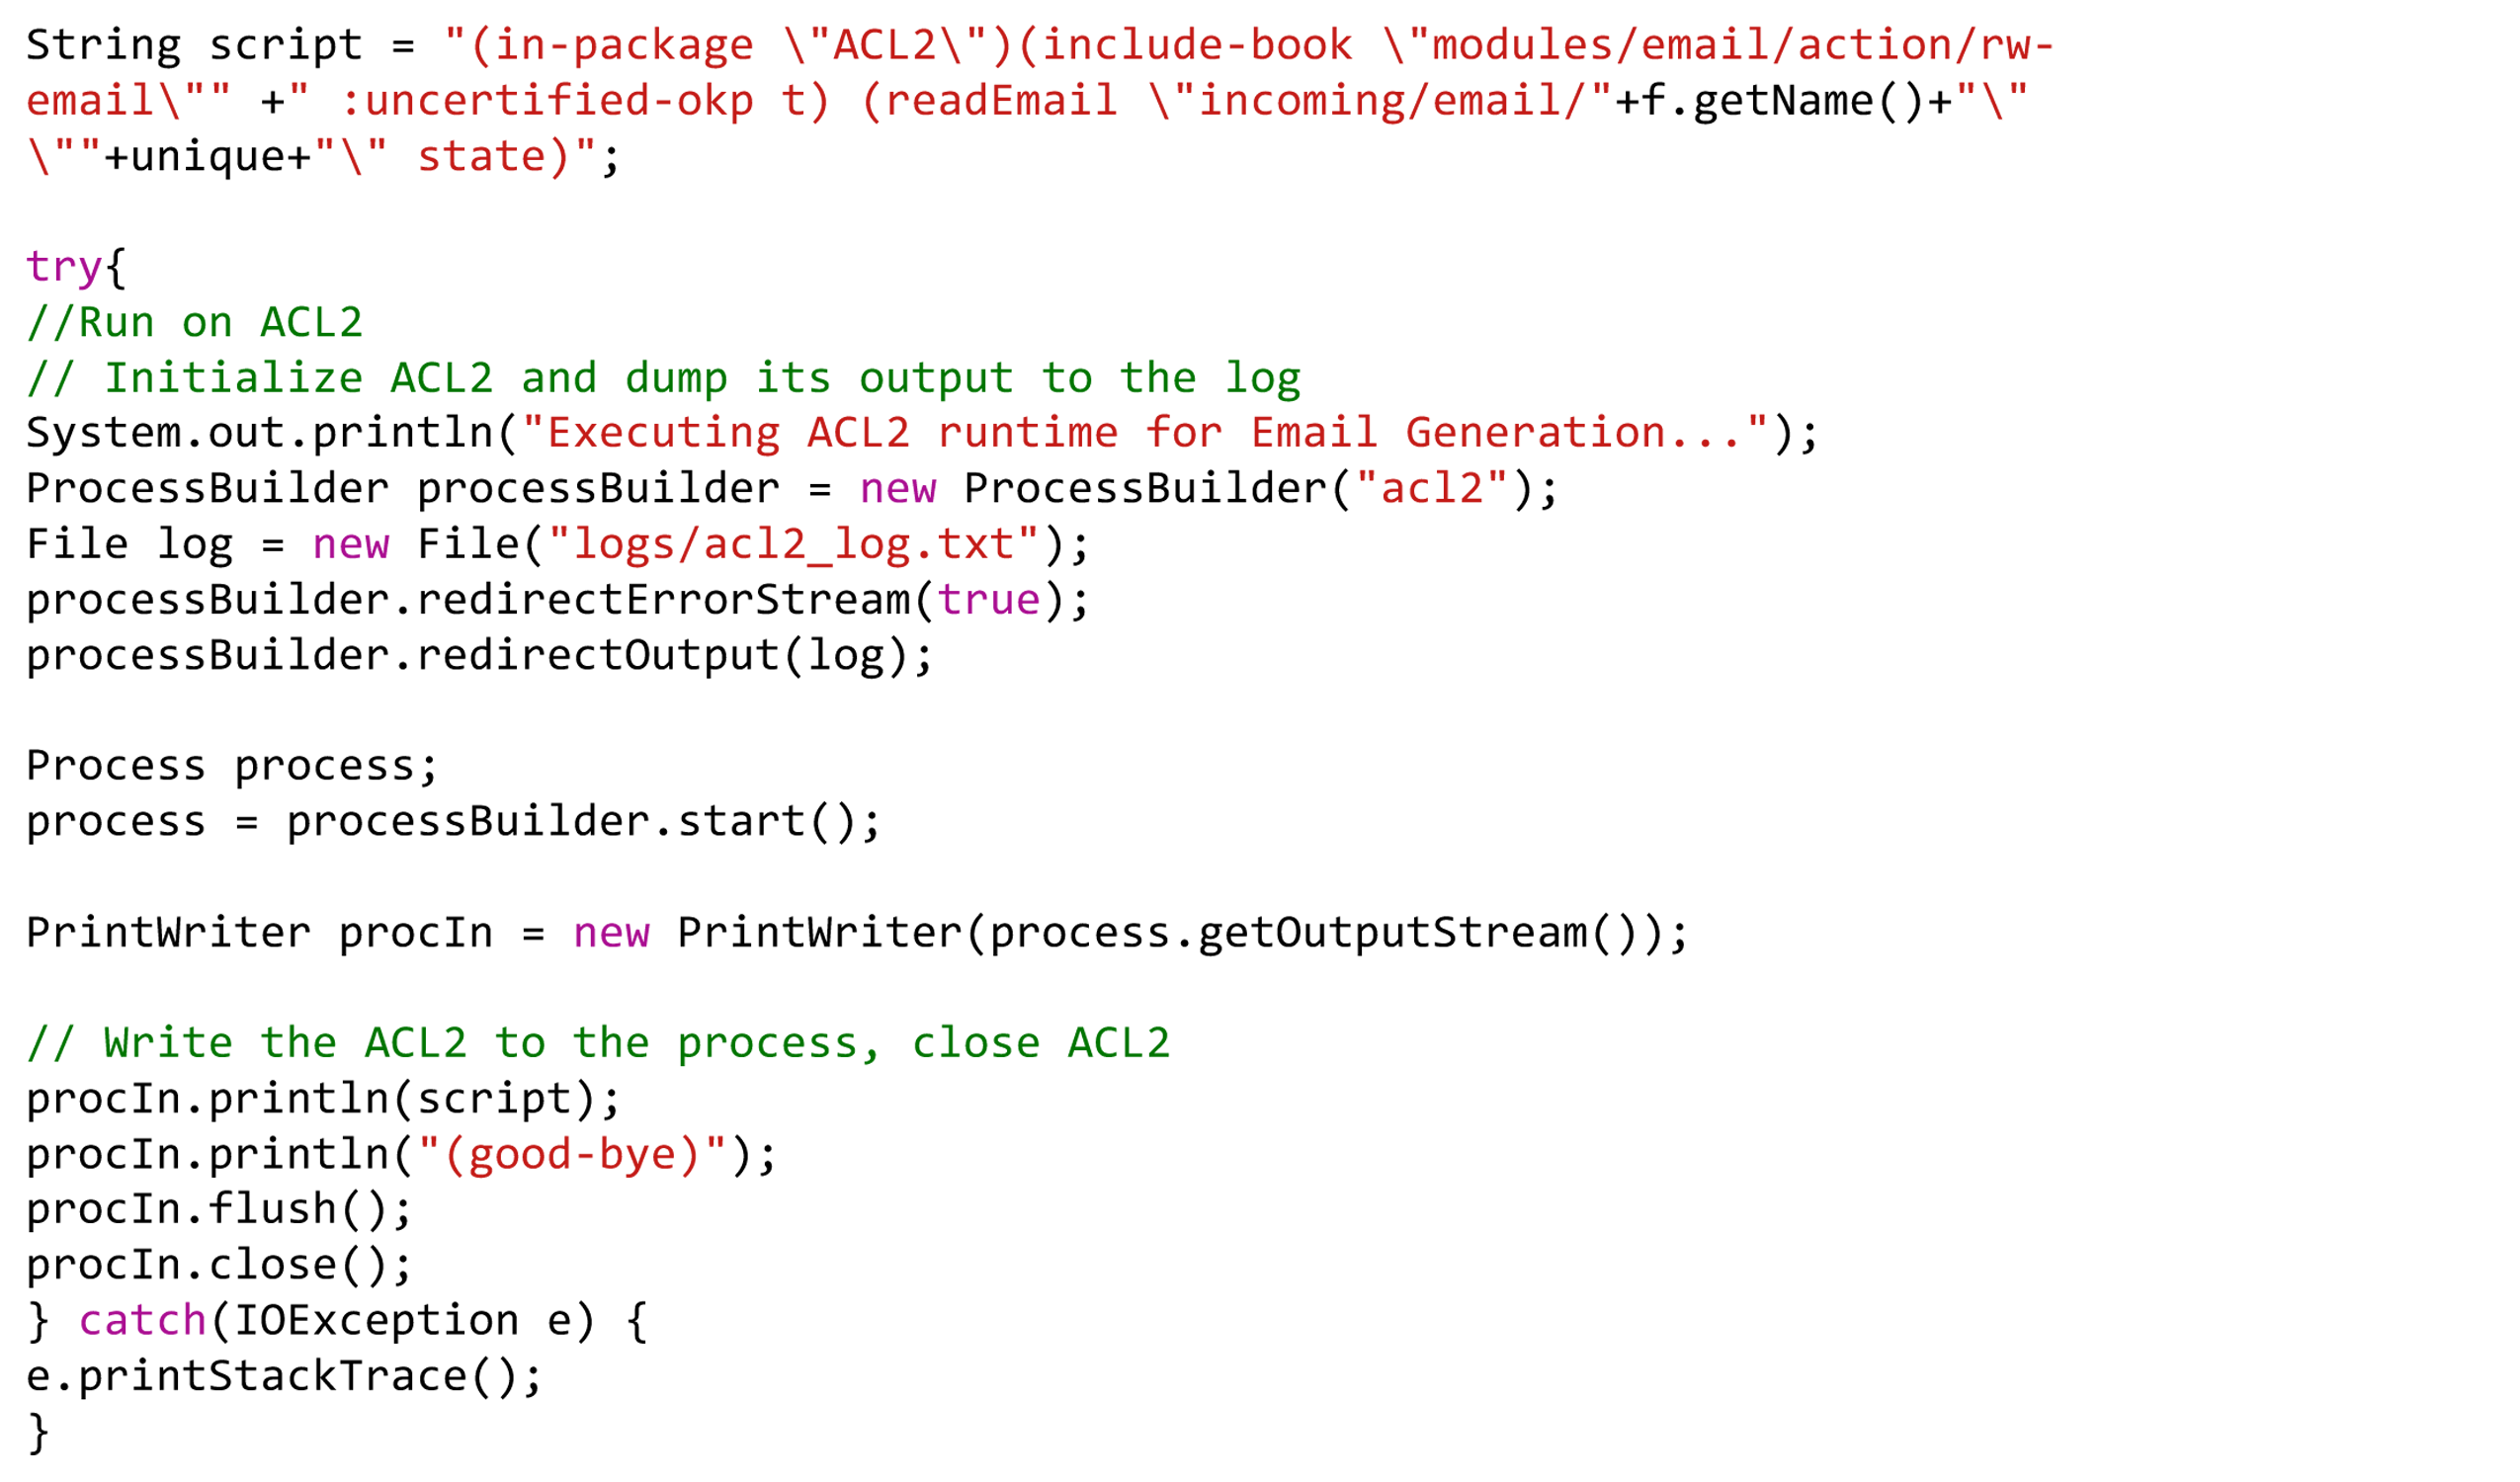
\includegraphics[scale=0.8]{javaproc}\\\\
This code will create a new process; call the ACL2 environment, and the build a string that is an ACL2 call to your ACL2 action file. The output of the ACL2 environment is then stored in a log folder in your client’s programs root directory. This is a way of seeing where the client program failed during debugging. \\
\item[The Module]\hfill \\
There are usually two parts to the to the action of a module. But it is possible to expand a module to more than two actions if it is needed to get a task completed. In order to explain the structure of a module, we will show the example of sending and Email message to the server. 

The action to be performed is email; a subfolder in the modules folder is created. This root folder, email, will contain the logic and test for the client-email platform. Within the email directory, another subfolder called actions is created. This folder will contain both the ACL2 actions and the Java actions for the email module. 

Since the execution of this module comes from the main root of the client application, we need to register the Java classes associated with sending emails with the following path: ``modules.email.action'' which makes the fully qualified name for invocation modules.email.action.sendEmail. We also need at least one lisp file in this directory which will contain the ACL2 IO functions needed to generate an email message to be sent. 

An example of one of these lisp files that will need to be included in the actions directory: 
\begin{verbatim}
(in-package "ACL2")

(include-book "../../../include/xml-scanner" :uncertified-okp t)
(include-book "../../../include/io-utilities" :uncertified-okp t)
(include-book "../client-email" :uncertified-okp t)
(set-state-ok t)

(defun writeEmailToFile (xmlStr to ts state)
  (mv-let (error state)
          (string-list->file (concatenate 'string 
                                          "store/email/outbox/"
                                          to ts ".xml")
                             xmlStr
                             state)
     (if error
         (mv error state)
         (mv "XML File Written Successfully" state))))


(defun writeMessage (to from sub msg state)
	(let* ((msgs (email to from sub msg)))
       (writeEmailToFile msgs to from state))
)
\end{verbatim}
This example lisp file will attempt to generate the XML file for the email message the user has inputted into the function \textit{writeMessage} and store it into the store/email/outbox directory on the client. \\

The input though, is first sent to the \textit{email} function in the client logic to generate the XML, if the user had addressed the email to multiple people, then the logic will handle the delegation of generating a list of multiple XML outputs. Once the logic has completed the function then saves the list of XML files in the outbox directory. \\

Once ALC2 has finished and saved the XML file in the Outbox, the Java process continues. It will open the file in the outbox and check the file to see if one or more XML messages are contained in the file. If more than one message is detected by using a regular expression, Java will split the file into multiple files such that only one message is included with each file and holding with the DTD definition. \\

Once the files are split, Java will send the messages to the server using a Java socket command. This is outlined in the Java program and is simple to implement. Most of the communications will occur on the following ports: 20002 for user verification, 20003 for user registration and 20005 for sending emails. Since we are sending an email, we will use port 20005 on the server to send the message.\\

This gives a basic overview of how the actions are performed in the client program. The other modules follow a similar pattern as sendEmail except each action has its own port as noted earlier. Once you complete a Java file, make sure you compile the \textit{.class} file in the same directory as the Java source code file. This will allow the action to be reachable from the root of the application and be used in other applications such as a GUI interface. \\
\item[The GUI]\hfill \\
Modules are invoked by a static method inside the modules Java library. This requires you to import the library in the Java program you are using. To import your Java library, you should use the import command using the path to your source code. This path should match the package name of your Java class. An example import would be:\\ \\
\verb$import modules.email.action.*;$\\\\
This will allow you to call the static action functions in the library and use the ACL2 modules from a Java program. For the \textit{sendEmail} example, you would call SendEmail.sendEmail(``To'', ``From'', ``Subject'', ``Message''). This will call the library and invoke the send email process in ACL2. 

By producing the Java programs in this fashion, we allow modularity of the program to remain independent of the GUI and other invocations. This has also allowed us to develop a stand-alone client GUI interface for the client. Once this is compiled on your machine. You will need to access the client directory from your command terminal. Once here you can issue the command:\\\\
\verb$java ACL2Email$\\\\
This will launch the Email client GUI interface. The current modules already imported into the interface are:
\begin{itemize}
\item Send Email
\item Verify User and Get Email
\item User Registration
\end{itemize}
Once more modules are developed; they can be easily implemented into this interface. With this structure, you are also able to make changes to the action files without having to worry about changing the GUI. The only action the GUI should make is to the static function in the actions library file. 



\newpage
\hypertarget{IO}{}
\item[\Large Input/Output] \hfill \\ 
\item[Email Message I/O] \hfill \\
The input and output for this project will be handled using XML data formatting. Each client connected
 to the server will be able to send email messages to the server. Messages sent to each client from
  the server should also use the same XML format for the message. Keeping this format for both
   outgoing and incoming messages will allow the client and server to use the same set of functions
    for reading and generating data. \\ \\
A sample of an XML email message output is listed below:
\begin{verbatim}
<?xml version="1.0"?>
<!DOCTYPE messages SYSTEM "email.dtd">
   <email>
        <to>wesley.howell@localhost</to>
        <from>matthew.crist@localhost</from>
        <subject>Message1 subject</subject>
        <content>Test For a Message Would be Here</message>
   </email>
\end{verbatim} 
The document type definition for this XML format is below:
\begin{verbatim}
<!ELEMENT email   (to, from, subject, content)>
<!ELEMENT from    (#PCDATA)>
<!ELEMENT to      (#PCDATA)>
<!ELEMENT subject (#PCDATA)>
<!ELEMENT content (#PCDATA)>

\end{verbatim}


\item[Email Address Book I/O] \hfill \\
The email address scheme for this project will be handled using the standard email format with the following modification. A sample email address for this project is:
\begin{center}\verb$name@domain$ \end{center}
The name portion of the email is the standard user name of the client on the domain. However, on the domain name, we have decided to drop the \verb$.com, .net, .org, etc.$ extensions since they will not be needed for this program's initial functionality. \\ \\
Email addresses are to be stored in an address book file which will have the following format.
\begin{verbatim}
<?xml version="1.0"?>
<!DOCTYPE addresses SYSTEM "address.dtd">
<addresses>
   <address>
        <domain>localhost</domain>
        <name>Matthew.Crist</name>
   </address>
   <address>
        <domain>localhost</domain>
        <name>Wesley.Howell</name>
   </address>
   <address>
        <domain>localhost</domain>
        <name>Adam.Ghodratnama</name>
   </address>
</addresses>
\end{verbatim}
The document type definitions for the addresses XML are as follow:
\begin{verbatim}
<!ELEMENT address* (name, domain)>
<!ELEMENT name (#PCDATA)>
<!ELEMENT domain (#PCDATA)>
\end{verbatim}

\item[Mailing List I/O] \hfill \\
Mailing list will also be stored to a file on the local machine/ server machine. The mailing list will allow one client to send a message to multiple clients. Also, a mailing list will need to be identified by its owner along with the email contacts to be stored on the list. \\ \\The structure of a mailing list file will be in the following XML format: 
\begin{verbatim}
<?xml version="1.0"?>
<!DOCTYPE mailing_list SYSTEM "mailing_list.dtd">
<mailing_list>
   <list_name>My mailing list</list_name>
   <addresses>
      <address>
         <domain>localhost</domain>
         <name>matthew.crist</name>
      </address>
      <address>
         <domain>localhost</domain>
         <name>wesley.howell</name>
      </address>
      <address>
         <domain>localhost</domain>
         <name>adam.ghodratnama</name>
      </address>
   </addresses>
   <owners>
      <owner>
         <name>matthew.crist</name>
         <password>my_password</password>
      </owner>
   </owners>
</mailing_list>
\end{verbatim}
The document type definitions for the Mailing List are as follow: 
\begin{verbatim}
<!ELEMENT addresses (address+)>
<!ELEMENT owners (owner+)>
<!ELEMENT list_name (#PCDATA)>
<!ELEMENT address (name, domain)>
<!ELEMENT name (#PCDATA)>
<!ELEMENT domain (#PCDATA)>
<!ELEMENT owner (name, password)>
<!ELEMENT name (#PCDATA)>
<!ELEMENT password (#PCDATA)>
\end{verbatim}

\newpage
\hypertarget{PROBE Estimates} {}
\item[\Large PROBE Estimates] \hfill \\ \hfill \\
During the initial design phase of this project, we created estimates based on our initial designs. The new objects section of the PSP++ report contain the information of these modules and the projected, detailed estimate for each object. 

The estimations provided were calculated using our team's Lines of Code table from the compilation of all the projects from the fall semester. \\ \\
The table is as follows:
\begin{table}[htdp]
\begin{center}
\begin{tabular}{lrrrrr}
Function Type & Tiny 7\% & Small 24\% & Medium 38\% & Large 24\% & Huge 7\% \\
\hline
Non IO Functions & 3 & 4 & 6 & 9 & 18 \\
IO Functions & 4 & 5 & 9 & 14 & 16\\
Properties & 3 & 4 & 6 & 8 & 14 \\
Check-Expects & 2 & 3 & 4 & 8 & 14\\
\hline
\end{tabular}
\end{center} 
\end{table}% 

Using this table, we were able to assign an estimated size of each function defined in this project. Each function is listed below along with the estimated size and Lines of Code for each particular function. \\ \\
Totaling all these functions, we are able to predict that this project will be around \textbf{1080} lines of new code. \\ 
We also need to note that the aim for this project is 2,500 - 3,500 lines of code. We can accept the 1080 line estimate because of the margin of error with the PROBE method. Since most of the projects that our team has completed mostly contained smaller scale functions, we can assume that the PROBE estimate can be off by a \textbf{factor of 3}. \\ \\
The PSP file that contains the objects used for the PROBE estimate are located in \textbf{Appendix A}. The summary of the new objects to be created are included with the following PSP++ report:

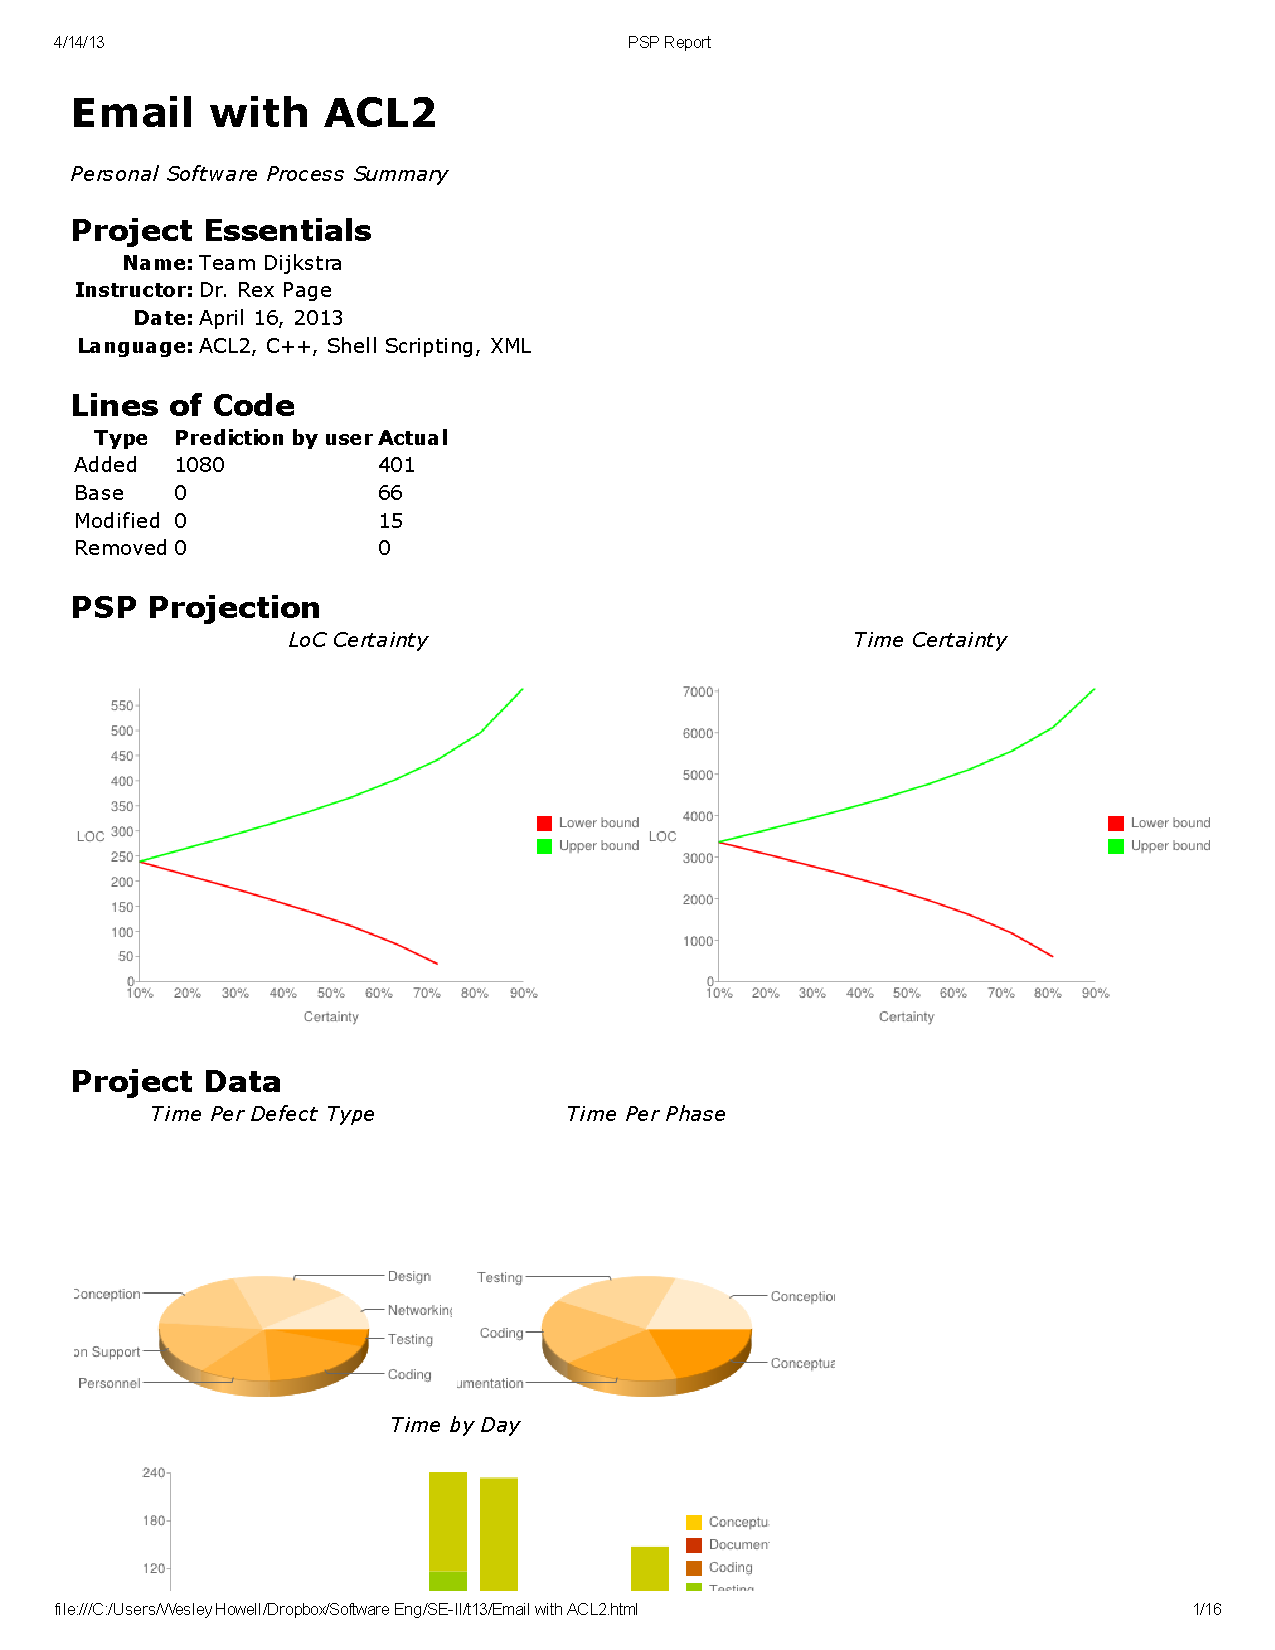
\includepdf[pages=1-16, pagecommand={}, scale=0.87]{PSPReport}


\newpage
\hypertarget{Additional Features} {}
\item[\Large Additional Features] \hfill \\ \hfill \\
The requirements mentioned so far in this project proposal are far from comprehensive. Numerous possibilities exist for expanding this project and adding additional features. In this section we will discuss extending the core features of the program. \\ \\These features outlined here, along with the original features that do not get implemented in the project will be available for the other groups in Software Engineering to implement. 
\item[Private Messaging with Attachments] \hfill \\ \hfill \\
This feature will extend each level of this project (i.e. Server, Client, I/O, and Networking). In order to implement secure messaging, we will need to setup facilities on the server to set up secure messaging. To do this we must add the following functions on the server.
\begin{itemize}
\item \textbf{isSecureMessage} - This function will parse the message's XML formatting to determine if the message is a secure message.
\item \textbf{postToSecureClient} - This function will send the secured messages to the proper secure clients and not the general population of unsecured clients.
\item \textbf{getSecureMessages} - This function will open the secured message buffers and act similarly to getClientMessages.
\item \textbf{getSecurityCredentials} - This function will obtain security credentials from the client to see if it is authorized to receive secure messages.
\item \textbf{authorizeSecureClient} - This function will take the client's user credentials and validate.
\item \textbf{registerSecureClient} - This function will register the client once the credentials are authorized.
\end{itemize}
The client program will do most of the work in the secured messaging. This allows for minimal server intervention and allows the messages to be encrypted as well. The client must perform the following functions:
\begin{itemize}
\item \textbf{isSecuredMessage} - This function will determine whether or not the most recently received message is a secured message.
\item \textbf{setSecuredType} - This function will set the secured output in XML format to the client's buffer.
\item \textbf{getSecuredOutput} - This function will parse a secured message's text format and return the function as a series of tokens.
\item \textbf{postSecuredMessage} - This function will post the secured message to the server's secure chat buffer file.
\item \textbf{inputEncryptionCode} - This function will take in the user's encryption key and use it to encrypt/decrypt messages.
\item \textbf{encryptMessage} - This function will encrypt the message.
\item \textbf{decryptMessage} - This function will decrypt a message.
\end{itemize} \newpage
In addition to secure messaging. The capability of secure attachments needs to be implemented. In order for attachments to be handled. The I/O XML format will need to be updated to accommodate an attachment tag. The secure attachment functionality will need these components:
\begin{itemize}
\item \textbf{openAttachmentFile} - Opens the attachment to send in a message.
\item \textbf{attachmentToBytes} - Converts the attachment to a byte stream.
\item \textbf{attachmentToXML} - Generates an XML tag for the attachment.
\item \textbf{addToBody} - Adds to the email message that an attachment is being sent.
\item \textbf{encryptAttachment} - Encrypts the attachments bytes for secure transmission.
\item \textbf{decryptAttachment} - Decrypts the attachments bytes.
\item \textbf{readAttachmentXML} - Reads XML metadata for the attachment.
\item \textbf{sendAttachmentToServer} - Sends the attachment to the server for forwarding.
\item \textbf{getAttachmentsFromServer} - Retrieves attachments from server.
\item \textbf{setAttachmentKey} - Sets the attachment's encryption key. 0 should be used for no encryption. 
\end{itemize}
The file used to generate the following PROBE estimate is attached in Appendix B. The PROBE estimate for this additional functionality is attached below:
\newpage
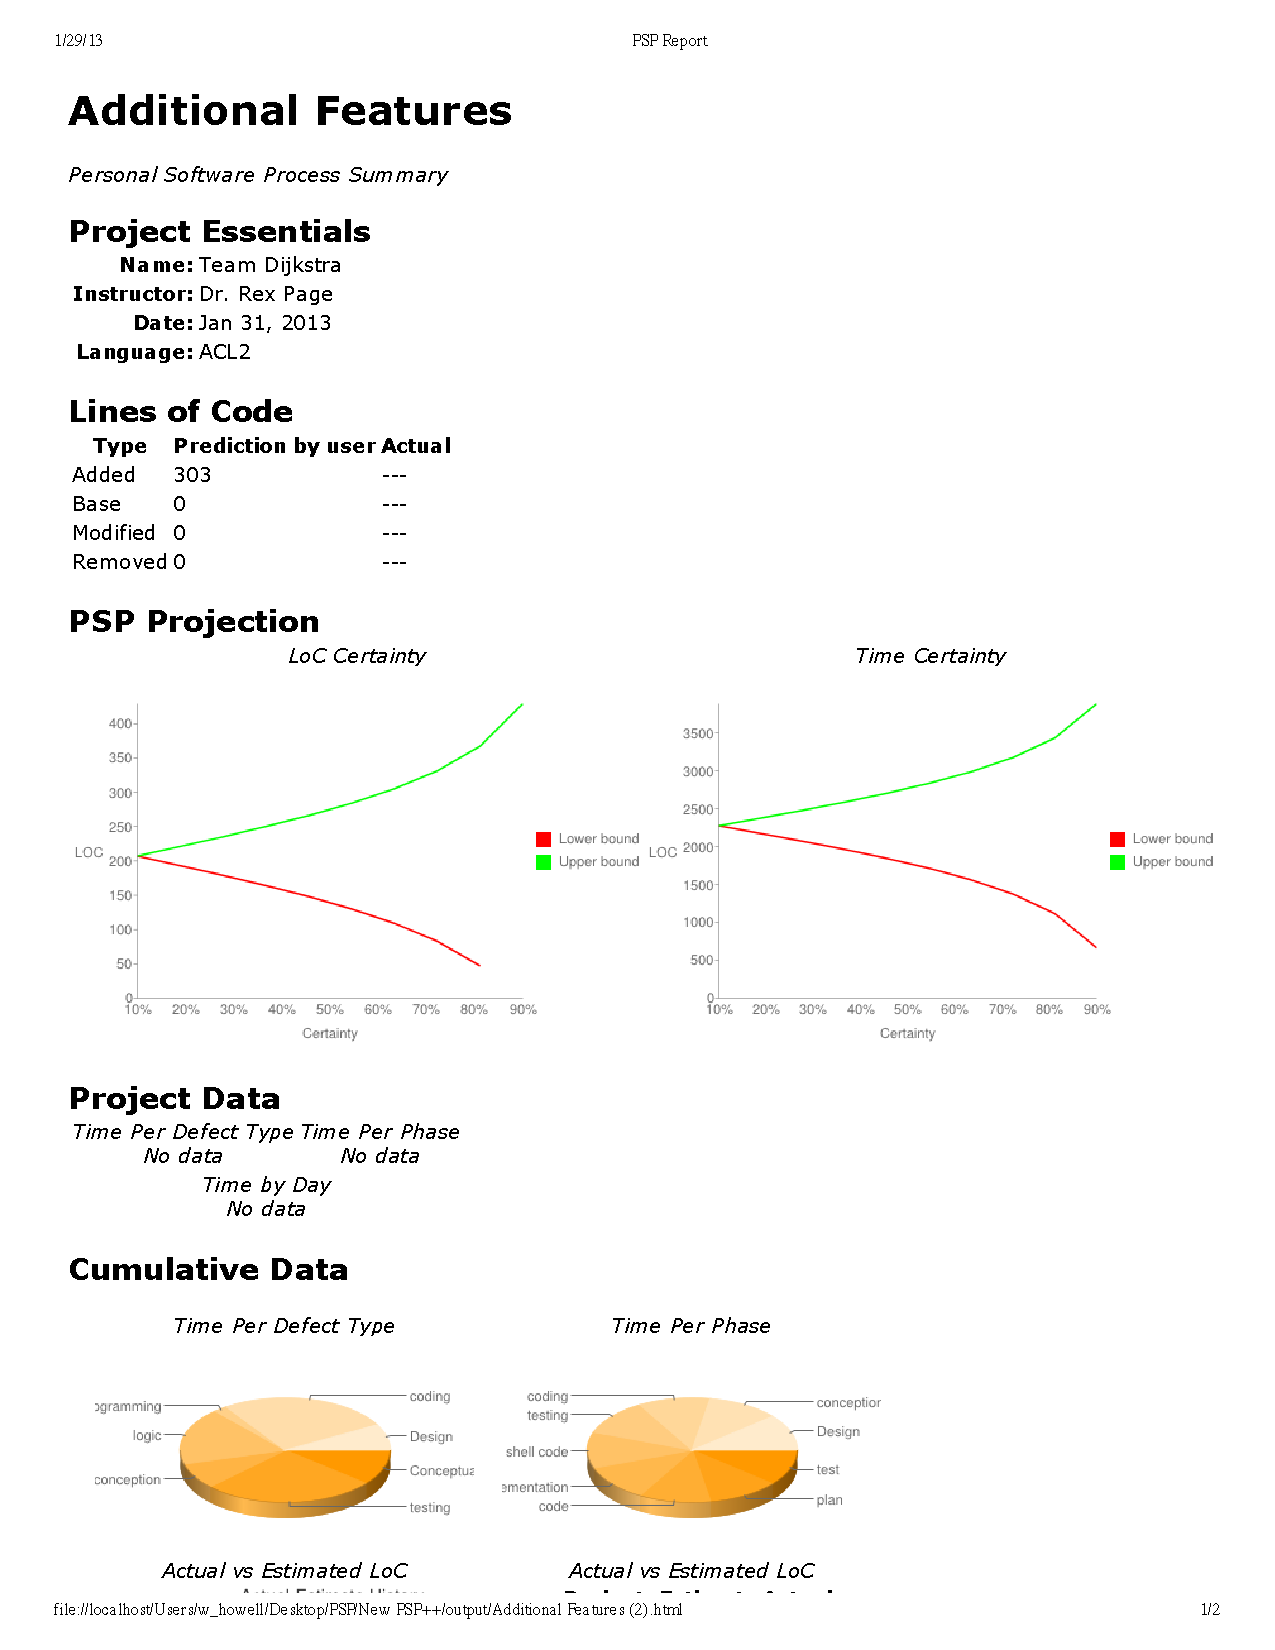
\includepdf[pages=1-2, pagecommand={}, scale=0.87]{PSPAdd}
\newpage
%\setcounter{page}{1}
%\pagenumbering{arabic}
%\rhead{Page A \thepage}


\hypertarget{Appendix} {}
\item[\Large Appendix]

\item[\large Appendix A: ACL2 Source Code Files] \hfill \\
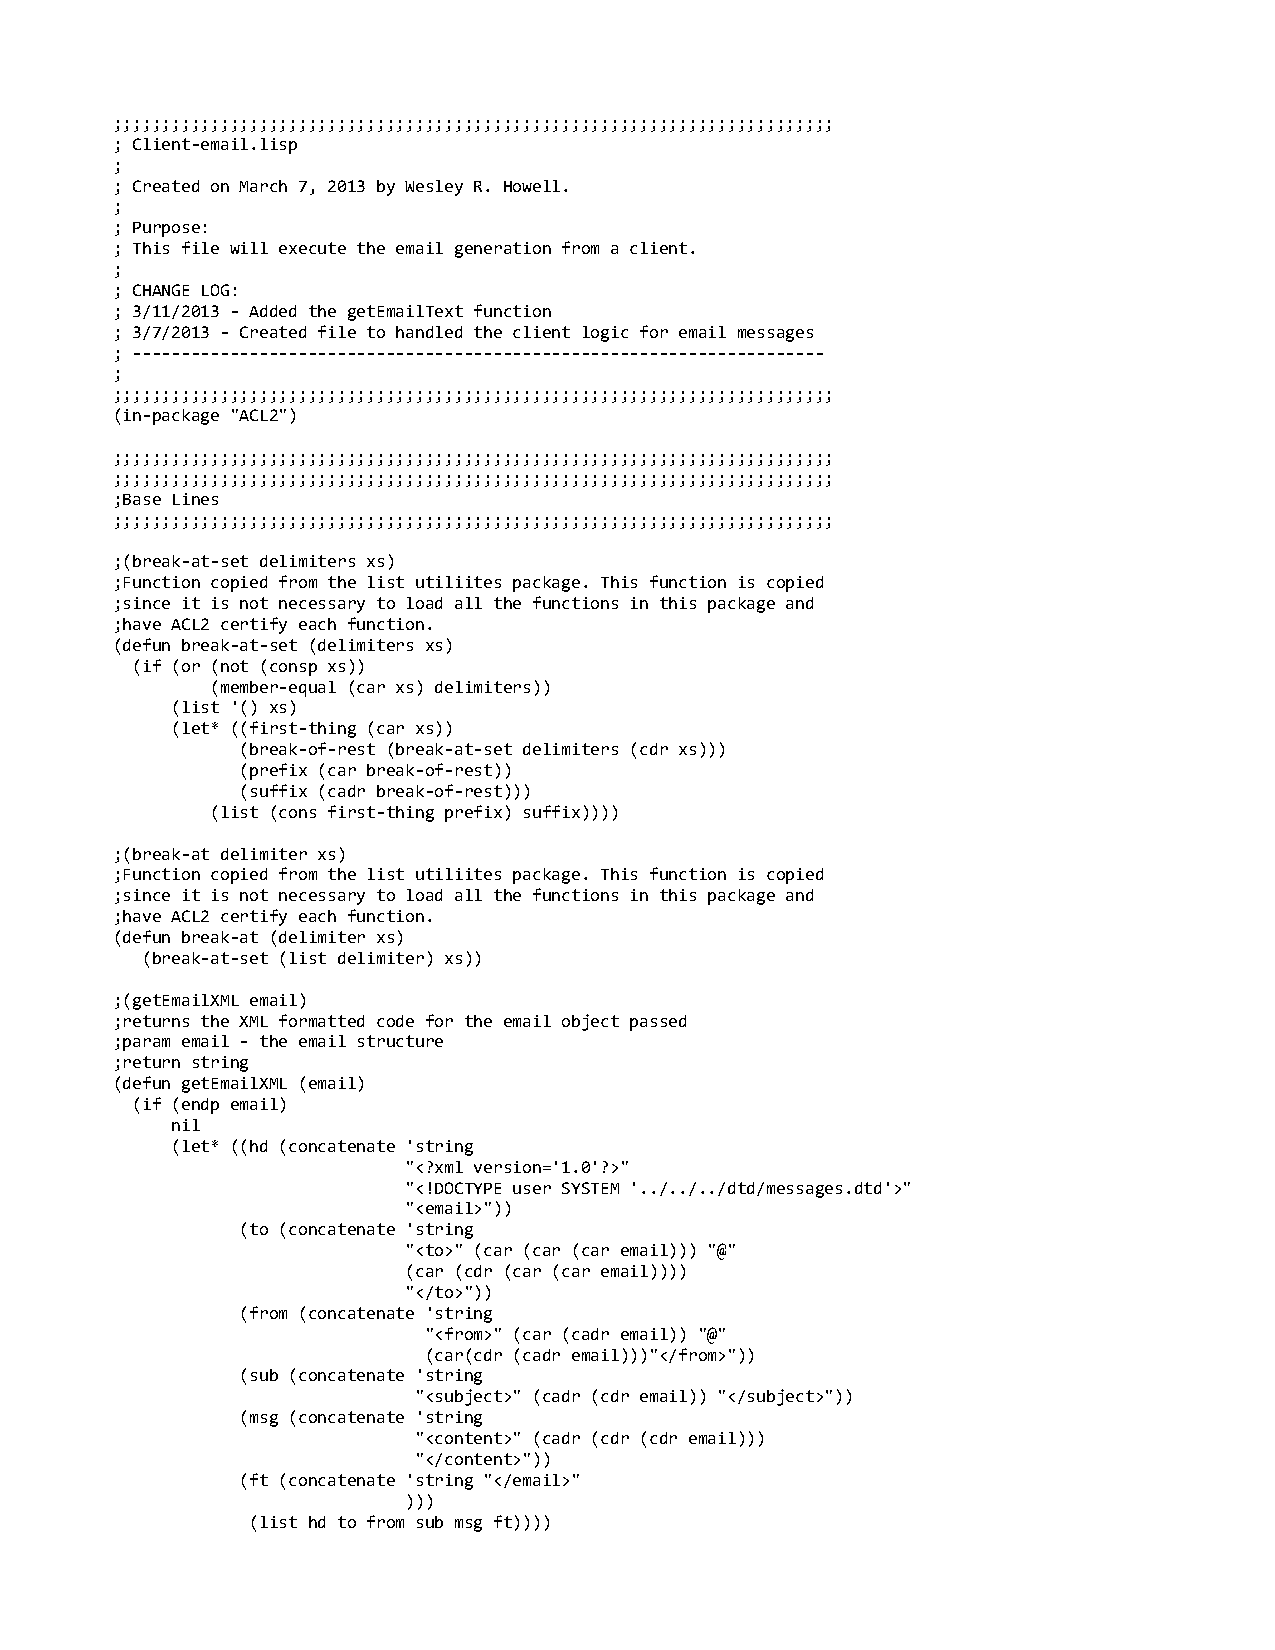
\includepdf[pages=1-3, pagecommand={}, scale=0.93]{client-email}
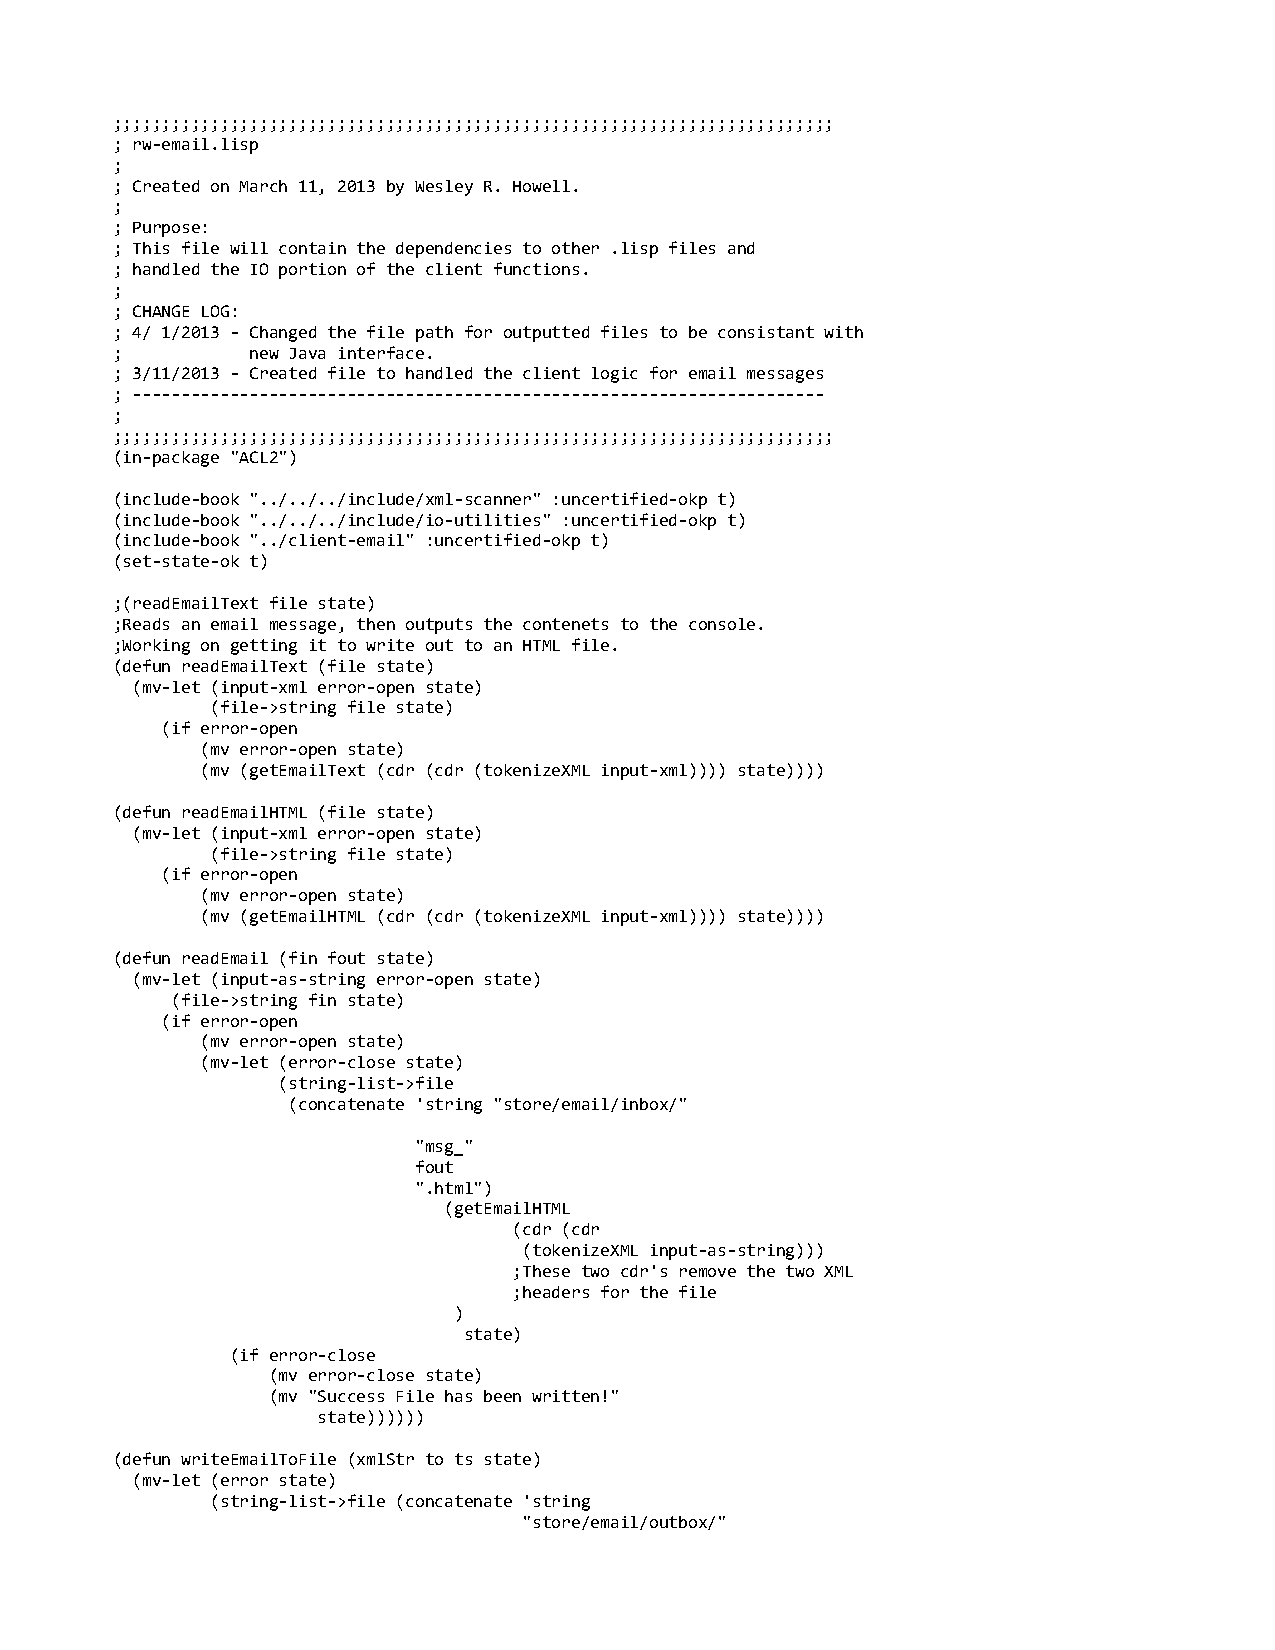
\includepdf[pages=1-2, pagecommand={}, scale=0.93]{rw-email}
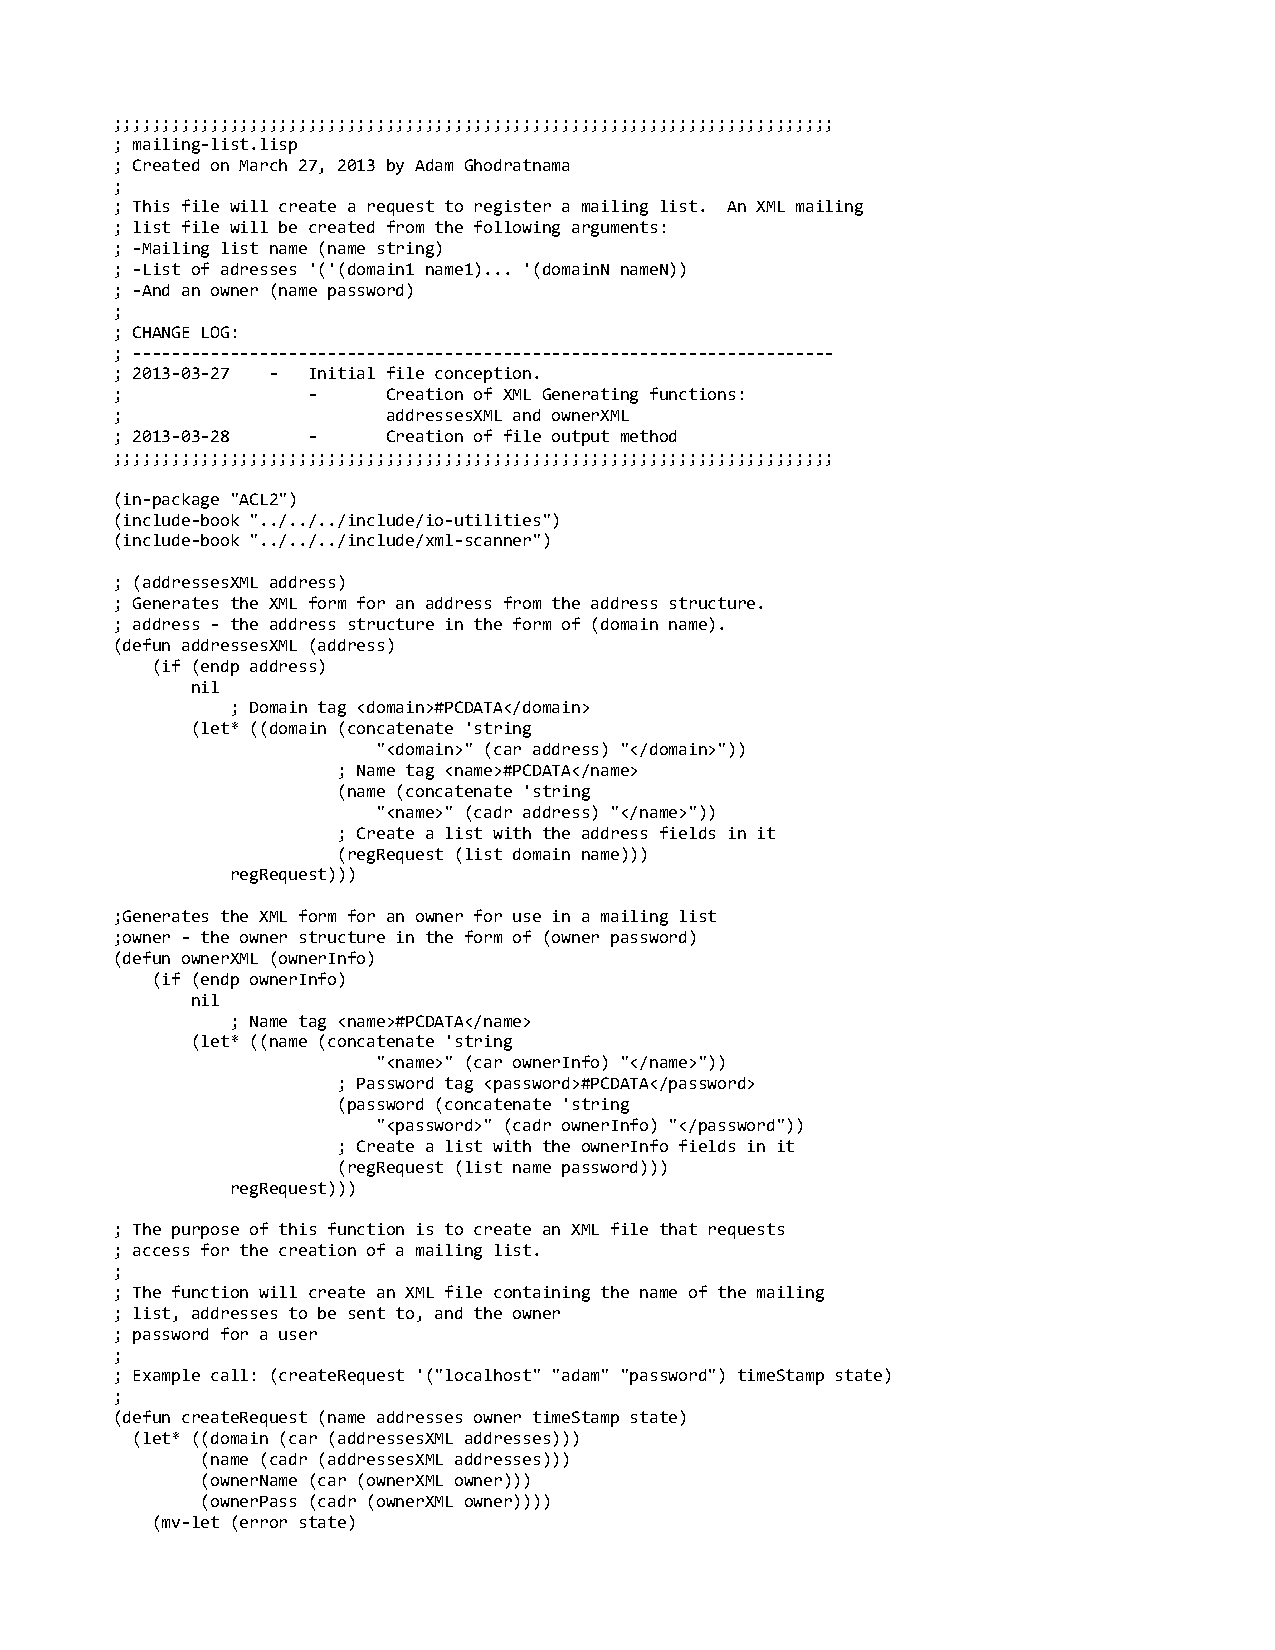
\includepdf[pages=1-2, pagecommand={}, scale=0.93]{create-mailing-list}
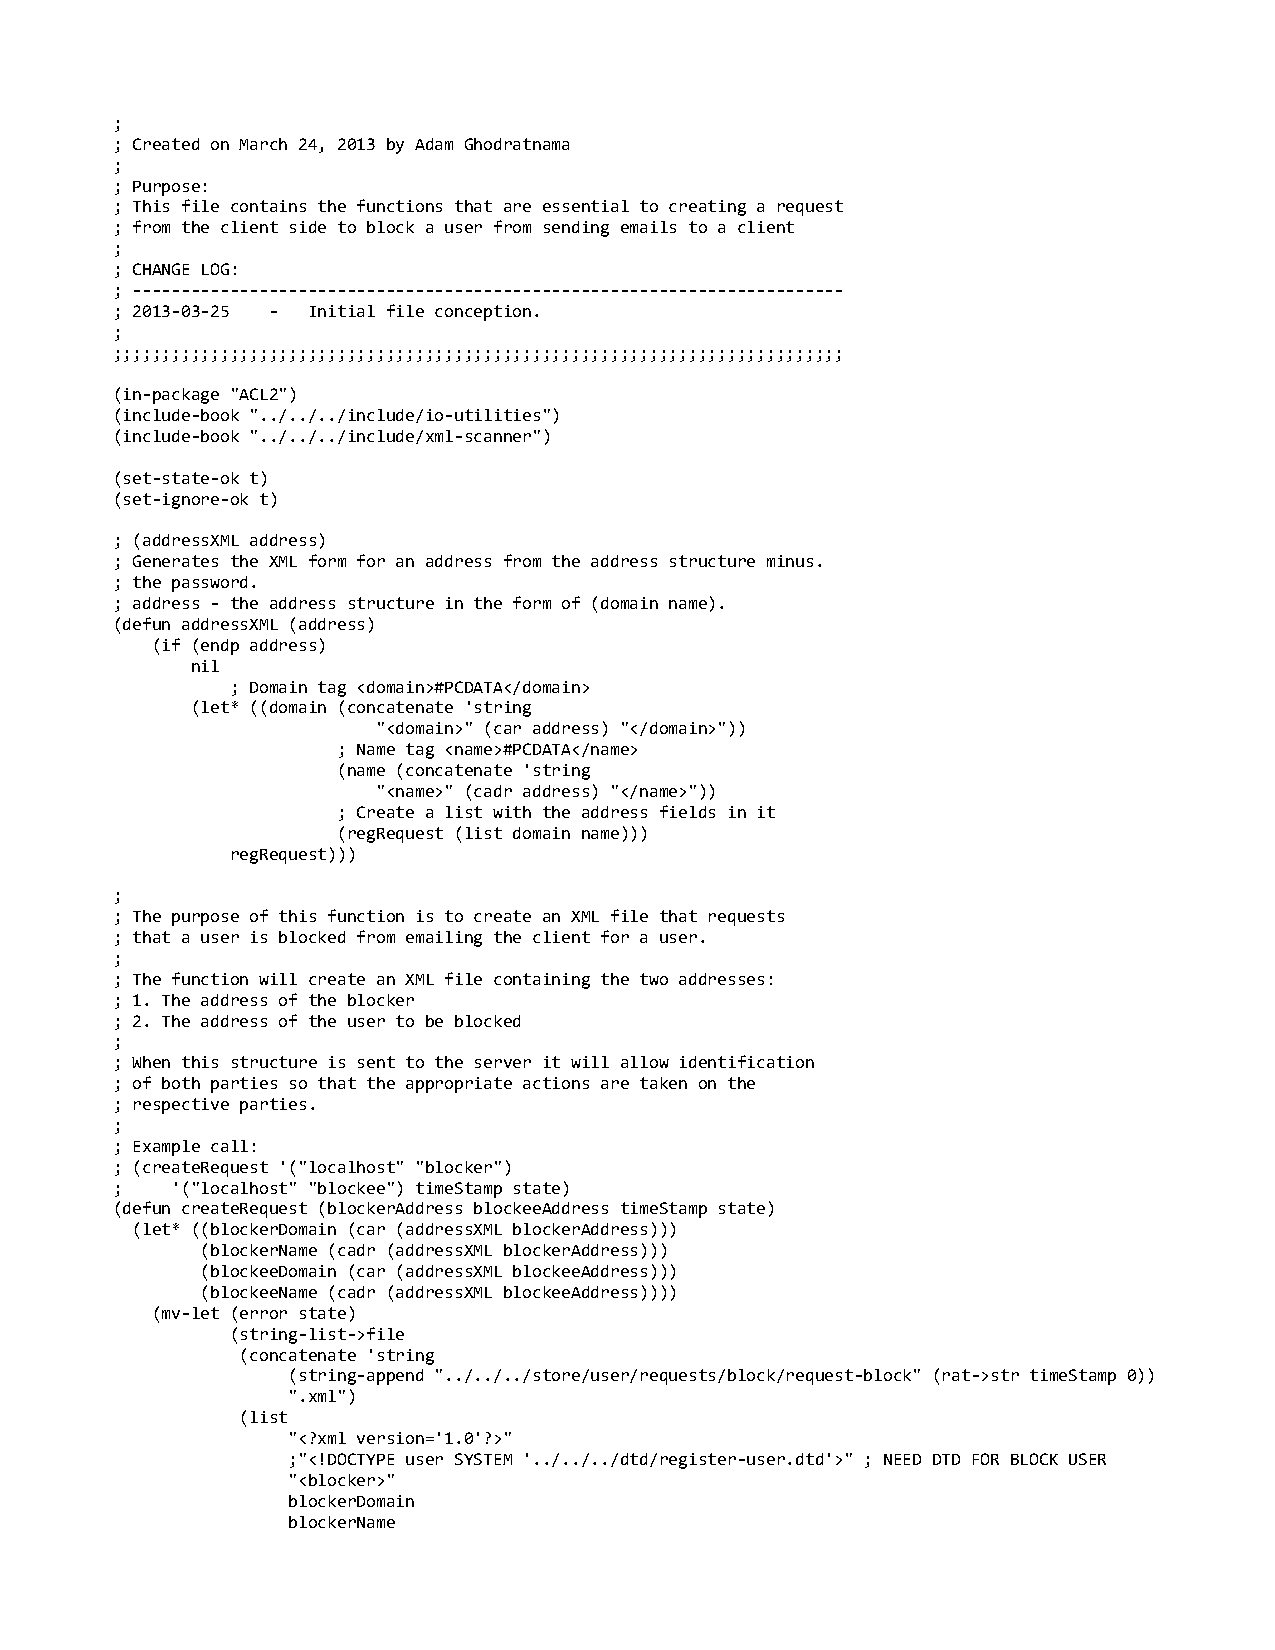
\includepdf[pages=1-2, pagecommand={}, scale=0.93]{create-block-request}
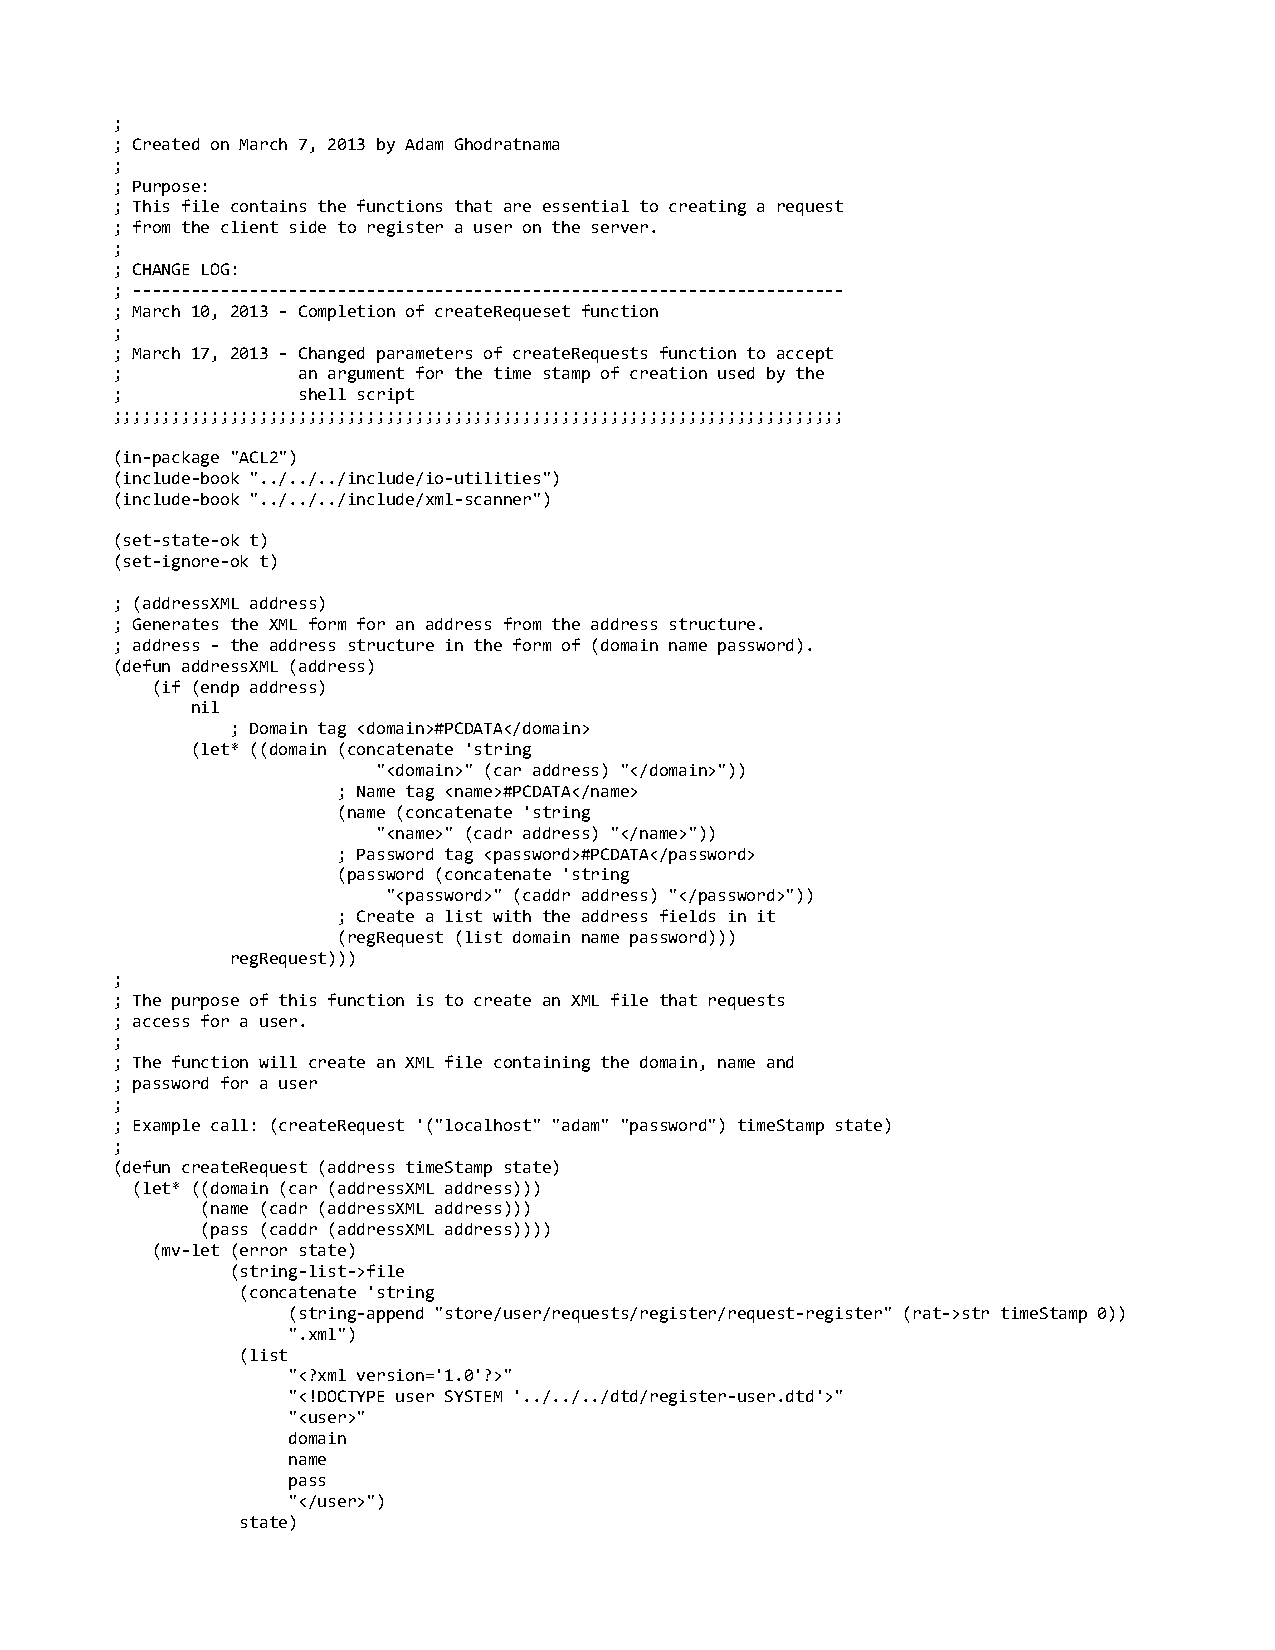
\includepdf[pages=1-2, pagecommand={}, scale=0.93]{create-user-request}
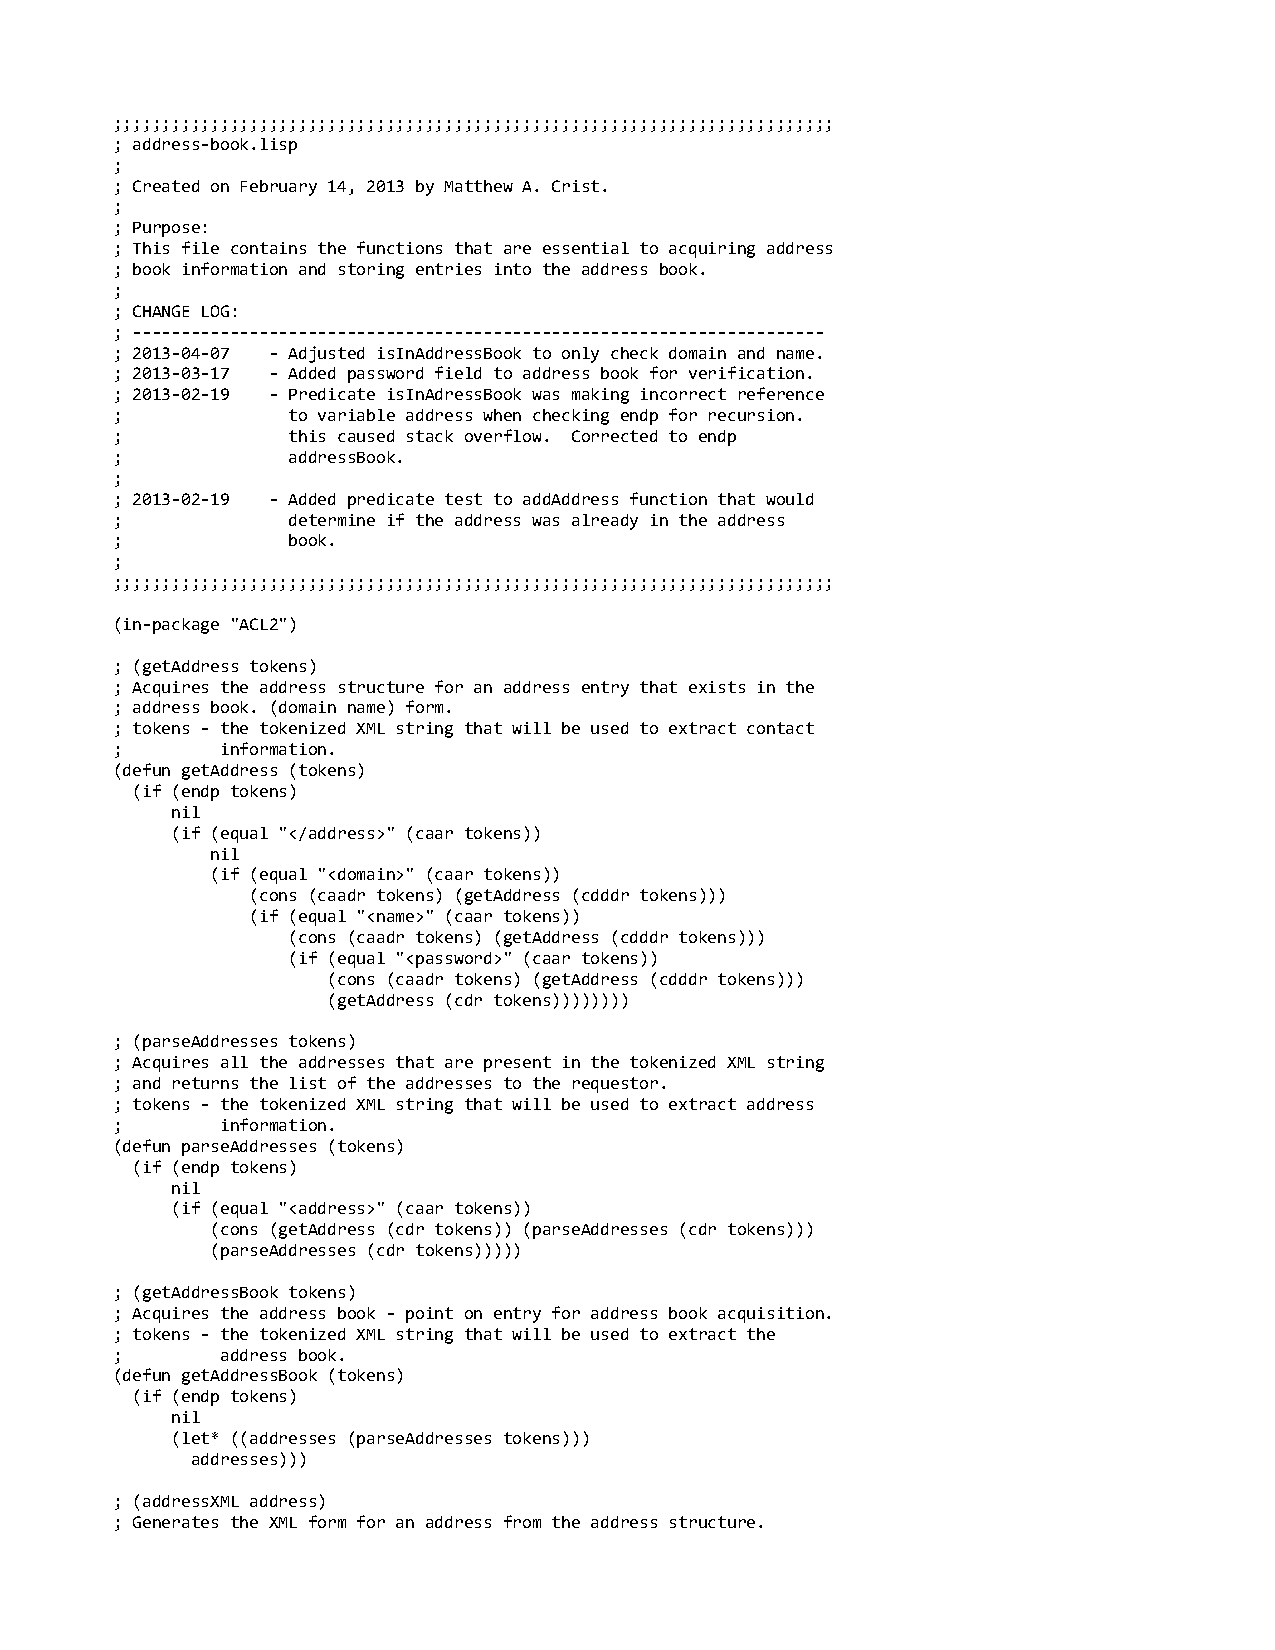
\includepdf[pages=1-3, pagecommand={}, scale=0.93]{address-book}
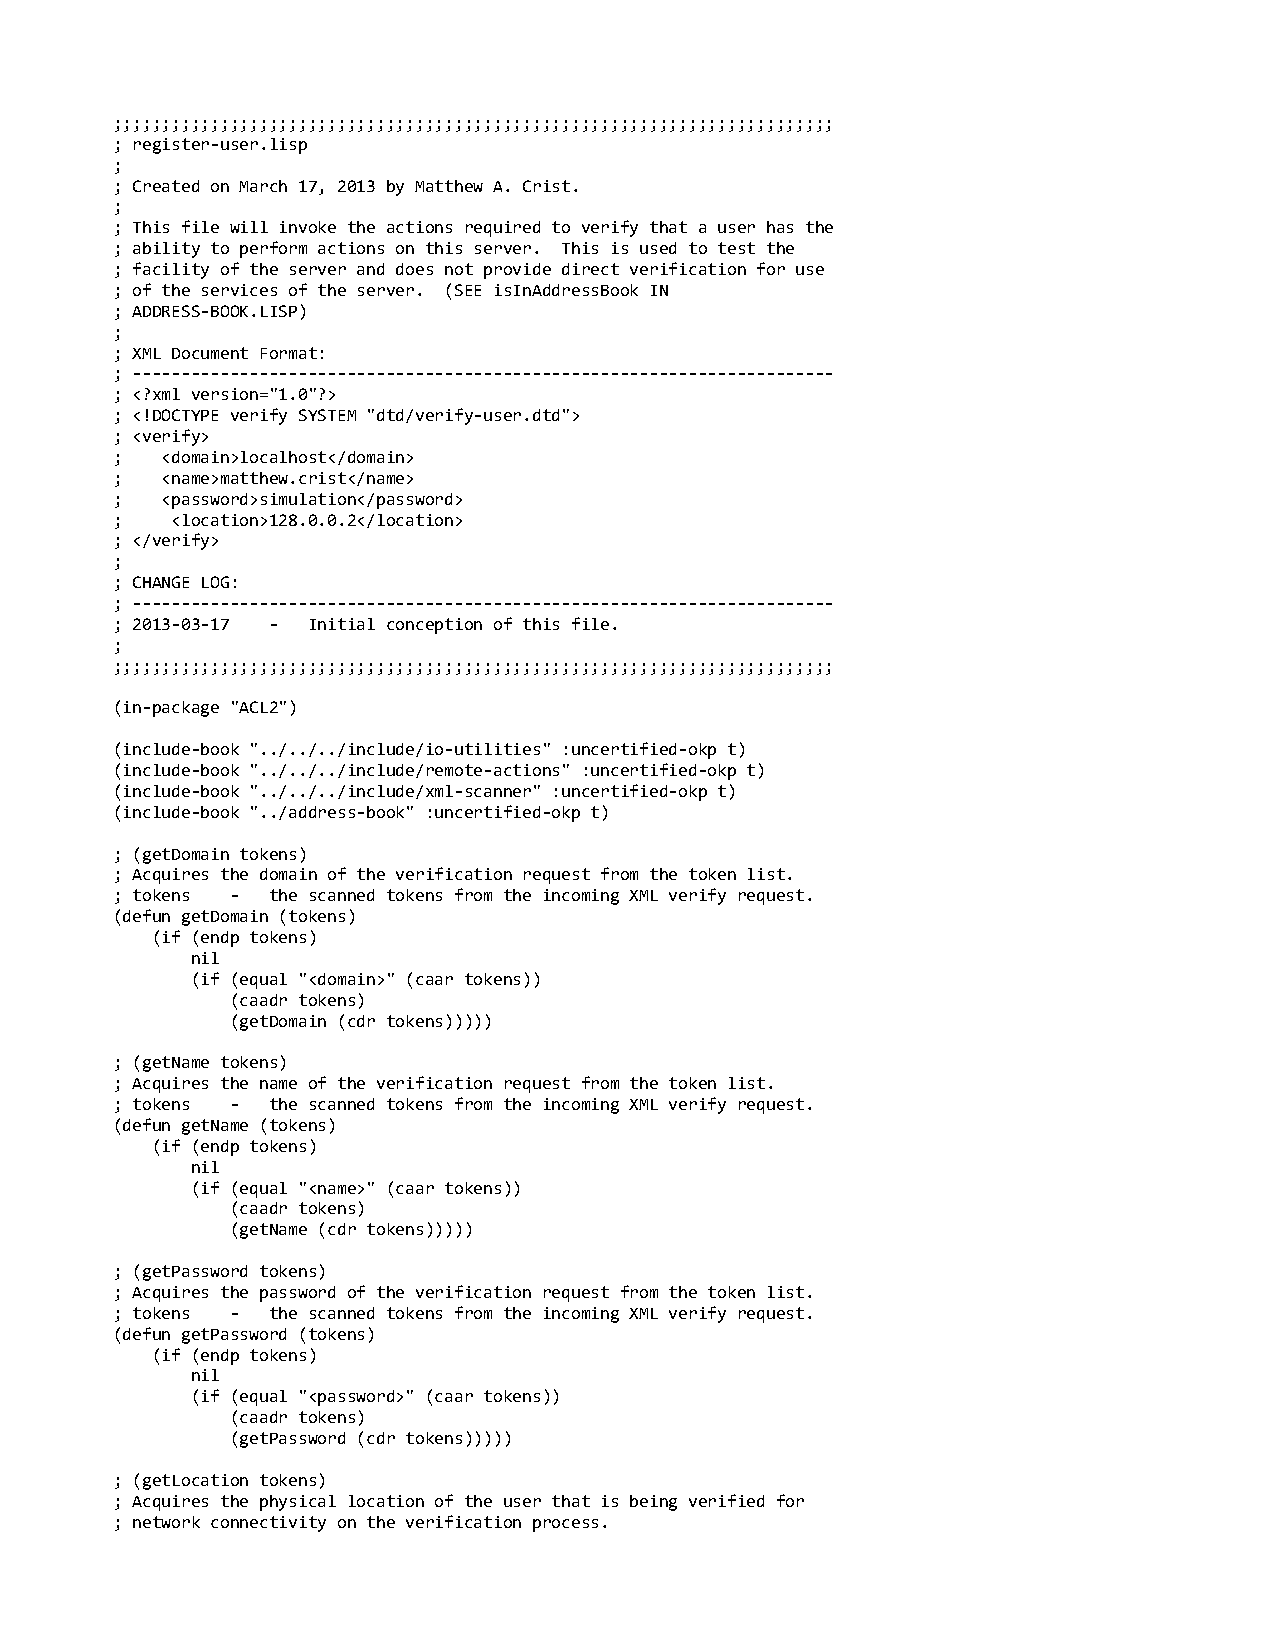
\includepdf[pages=1-2, pagecommand={}, scale=0.93]{verify-user}
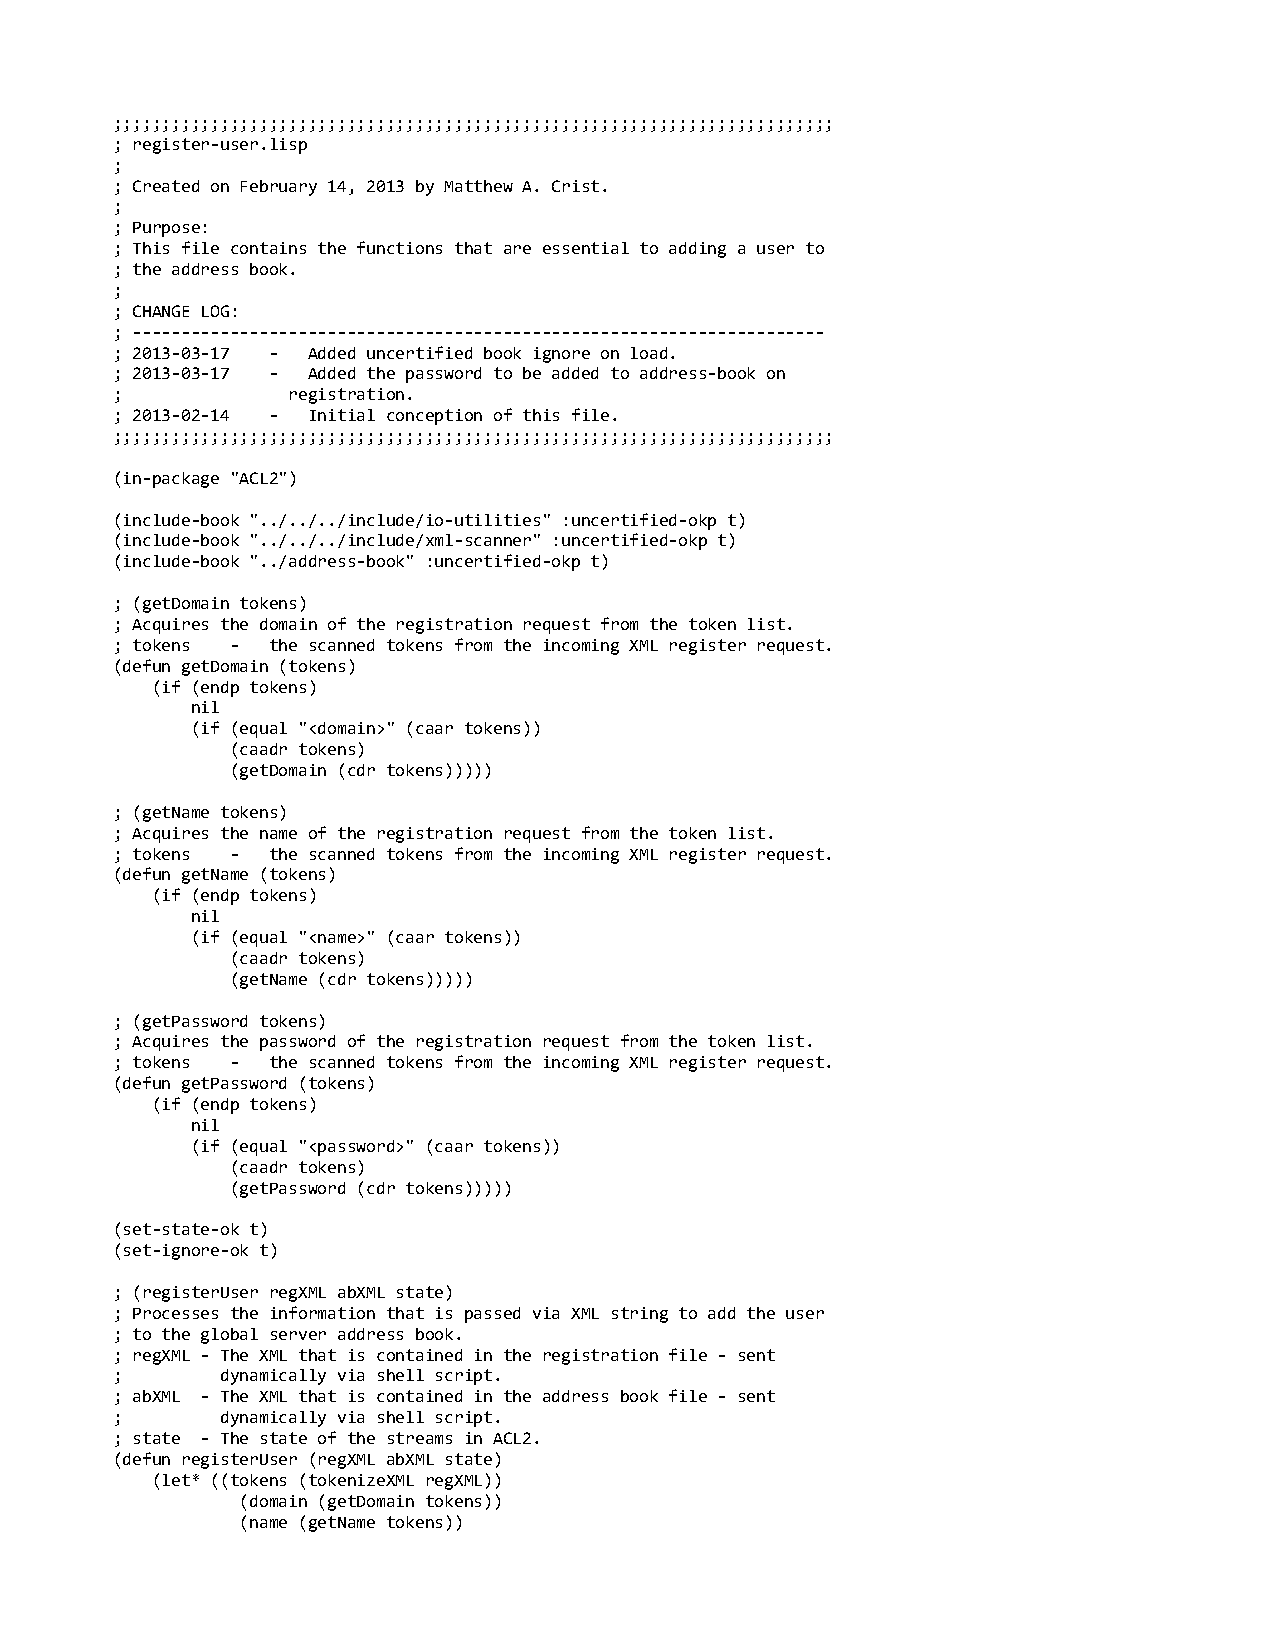
\includepdf[pages=1-2, pagecommand={}, scale=0.93]{register-user}
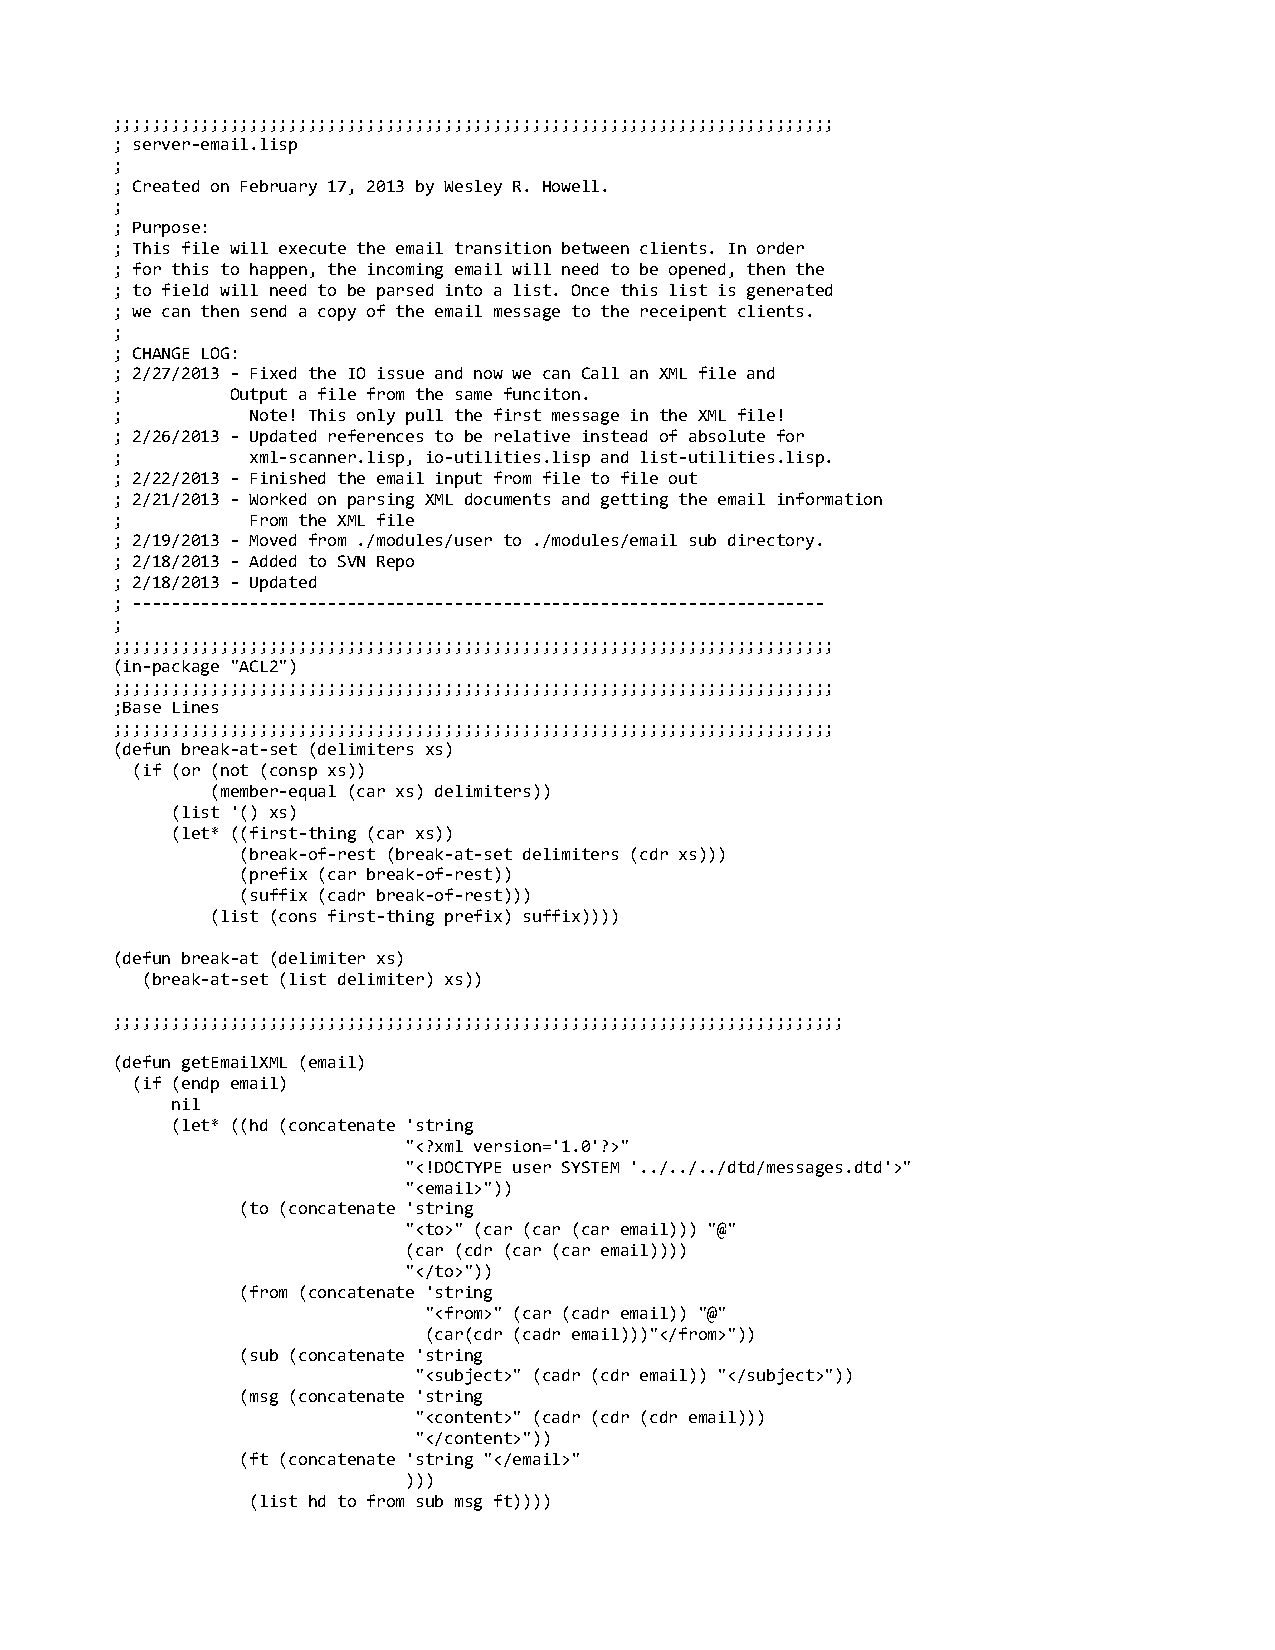
\includepdf[pages=1-2, pagecommand={}, scale=0.93]{server-email}
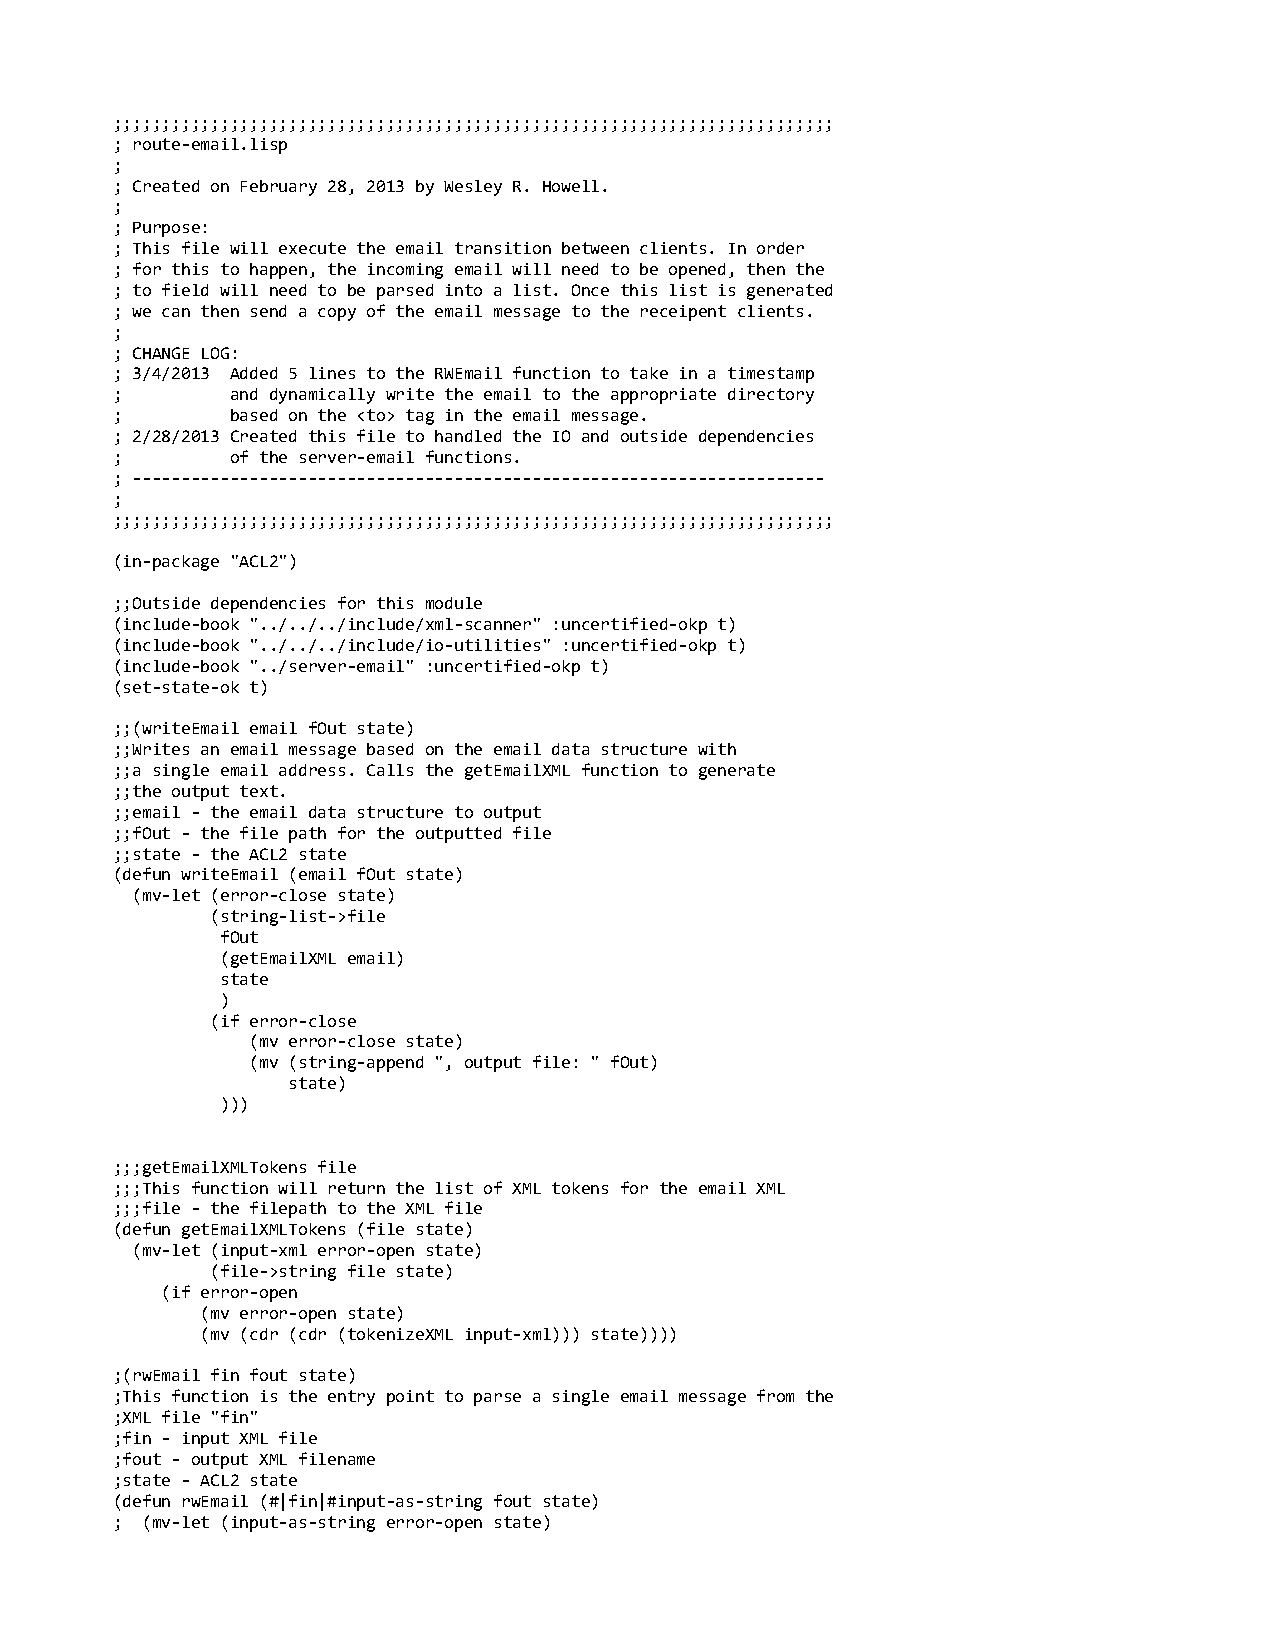
\includepdf[pages=1-2, pagecommand={}, scale=0.93]{route-email}
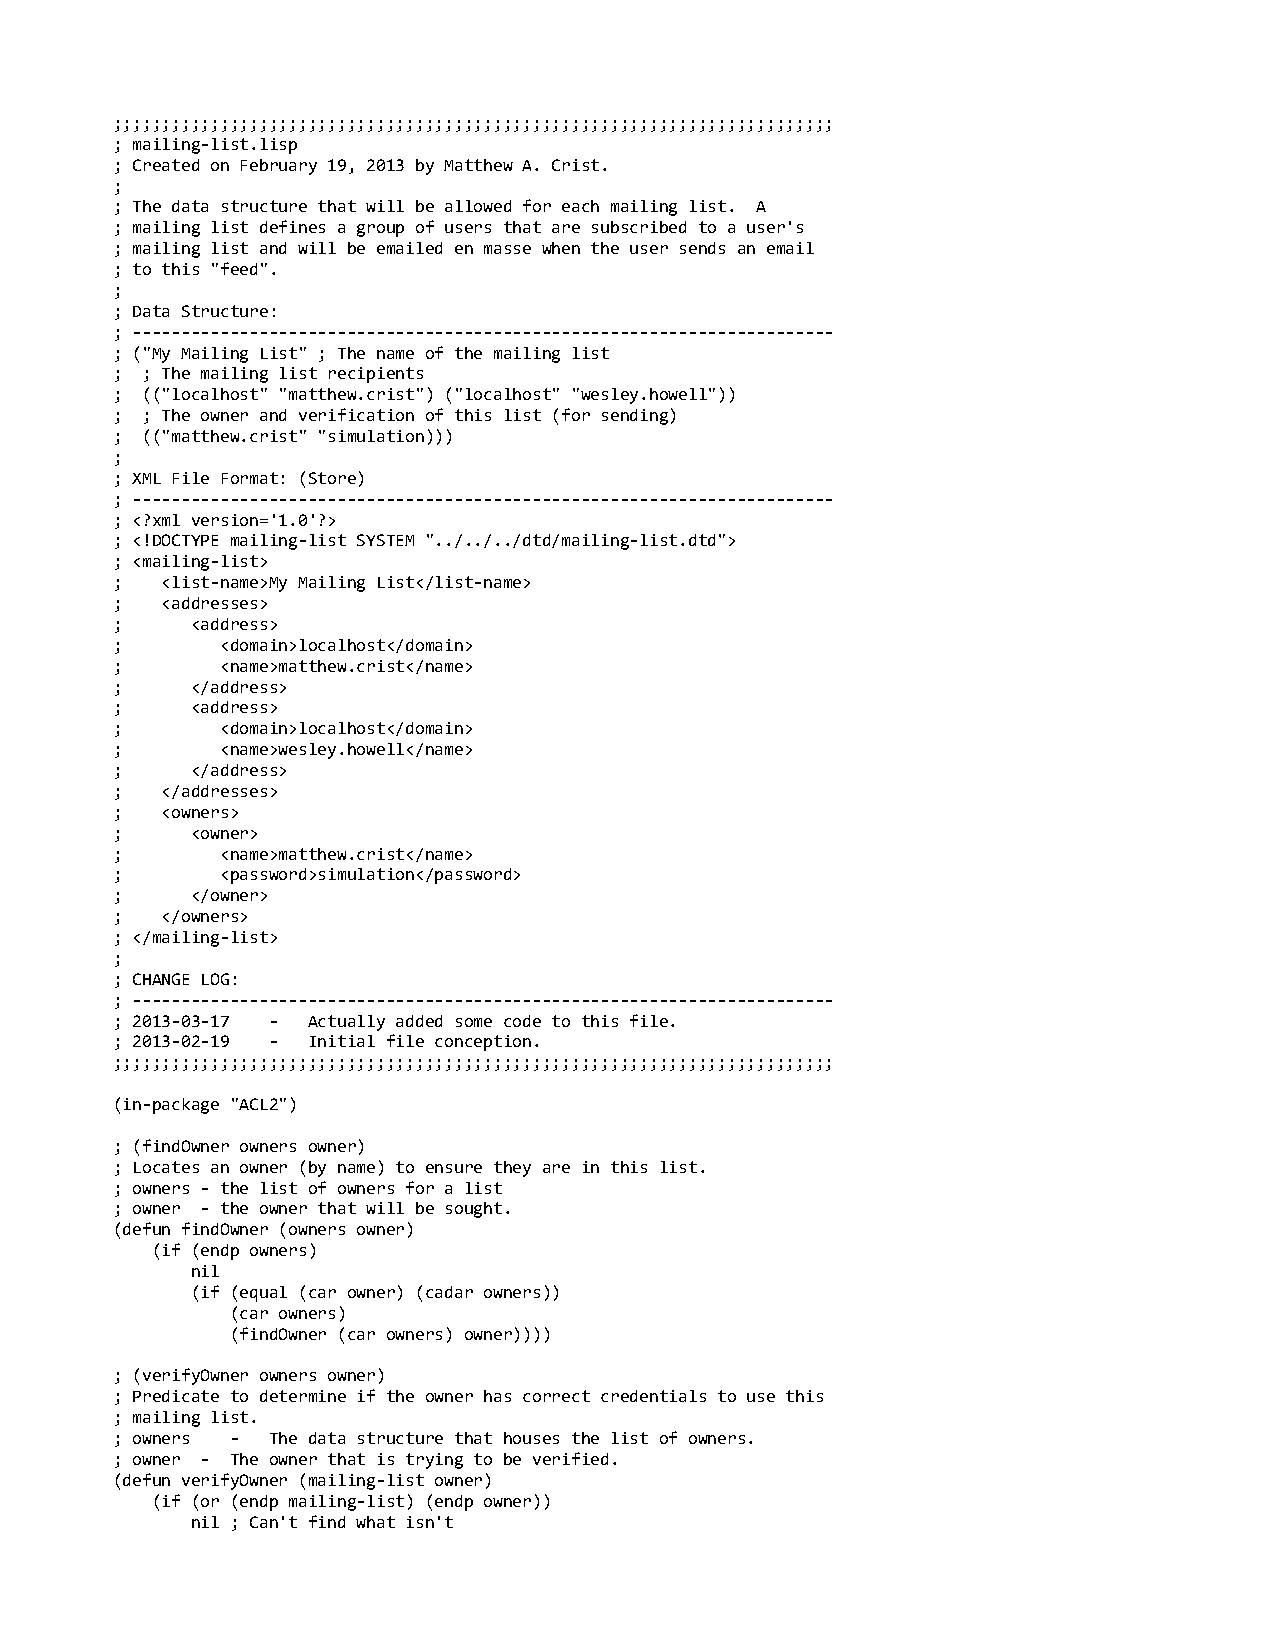
\includepdf[pages=1-4, pagecommand={}, scale=0.93]{mailing-list}

\item[\large Appendix B: ACL2 Test and Theorem Files]\hfill \\ 
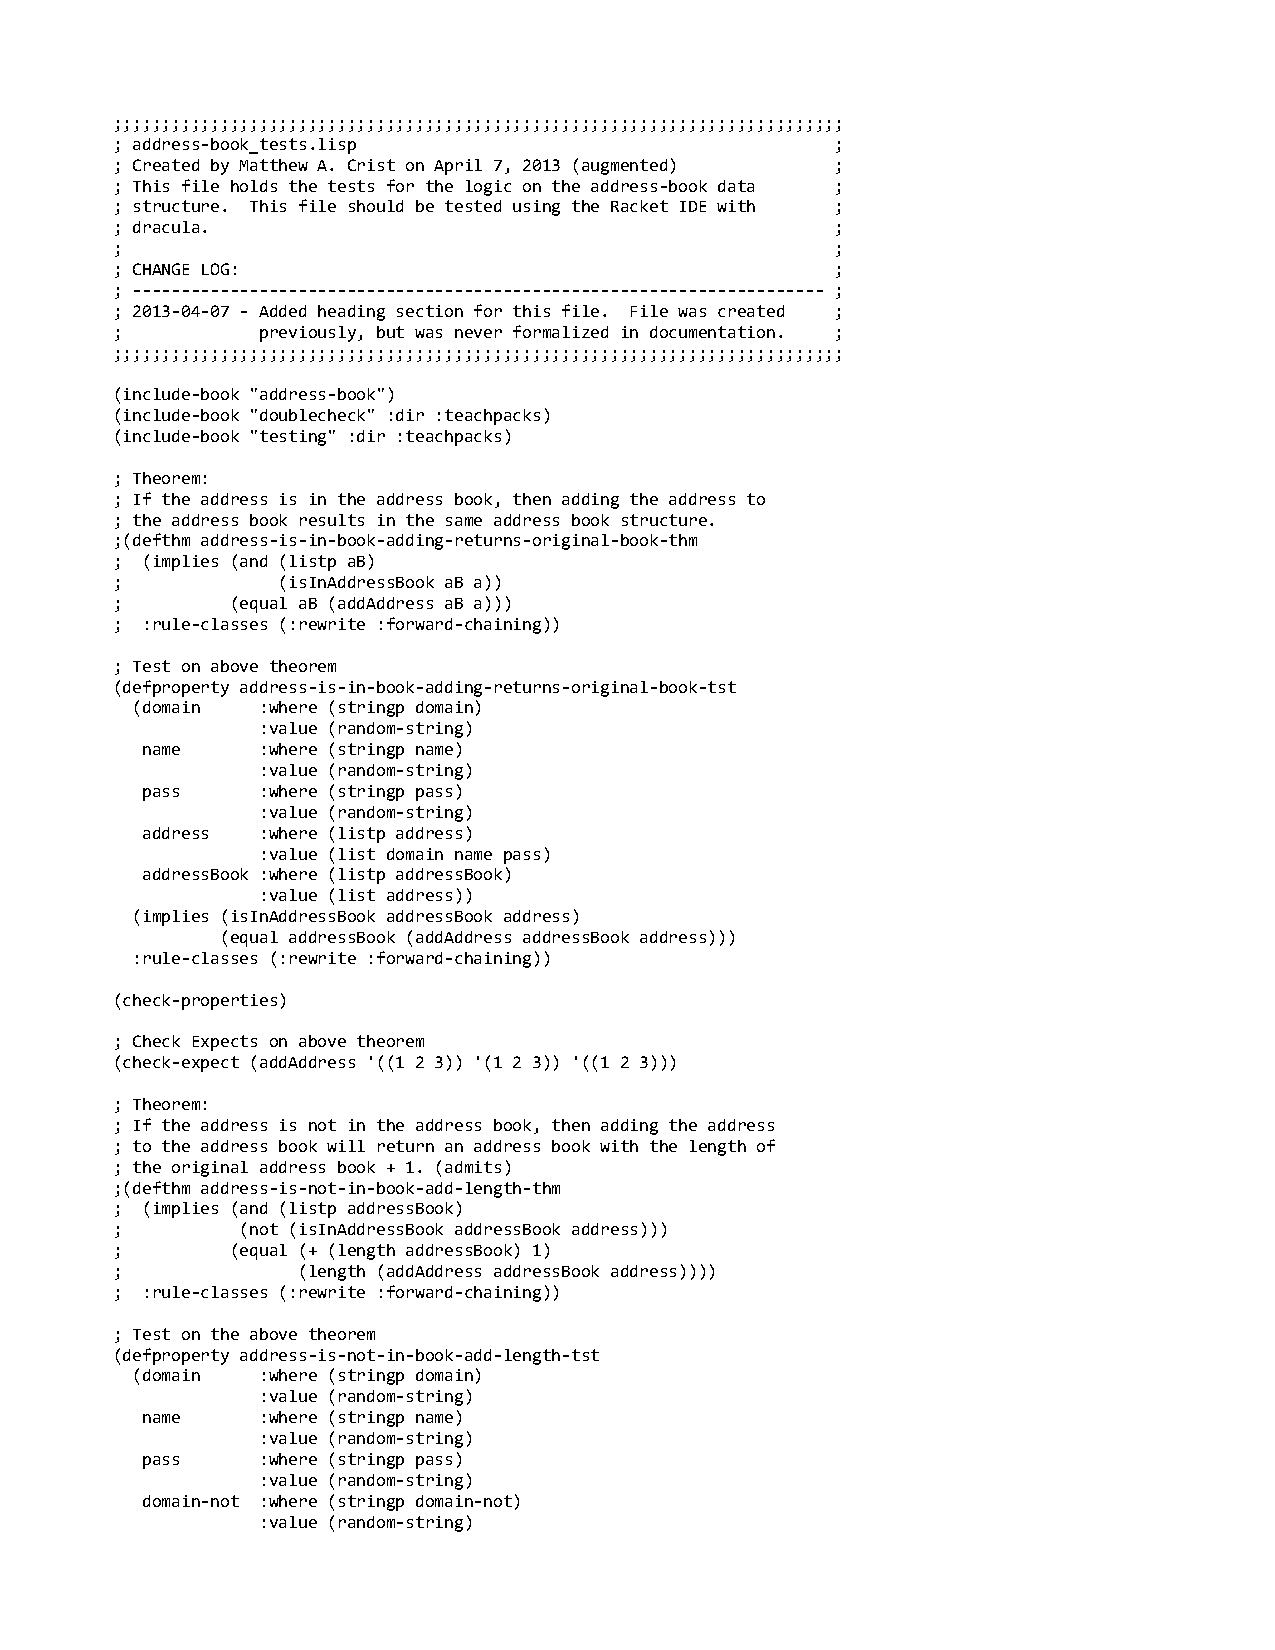
\includepdf[pages=1-3, pagecommand={}, scale=0.93]{address-booktests}
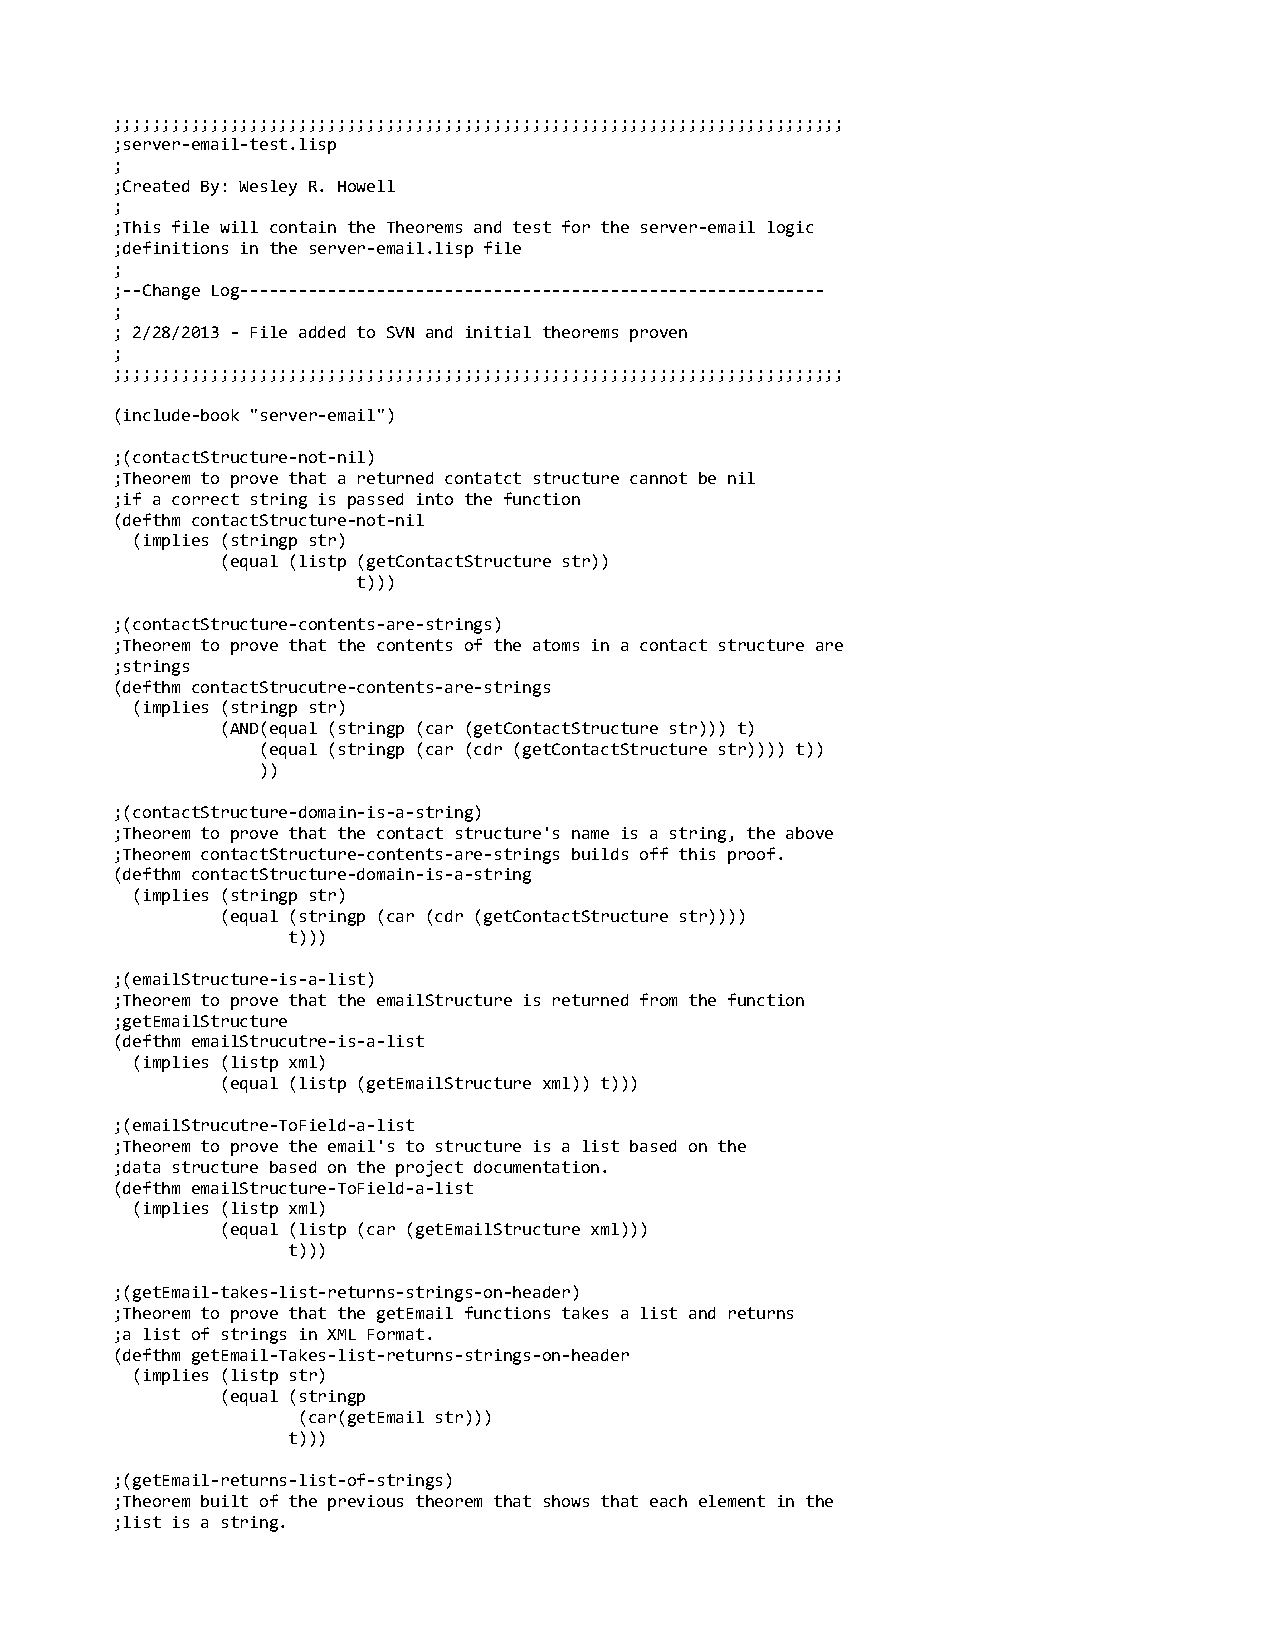
\includepdf[pages=1-2, pagecommand={}, scale=0.93]{server-email-test}
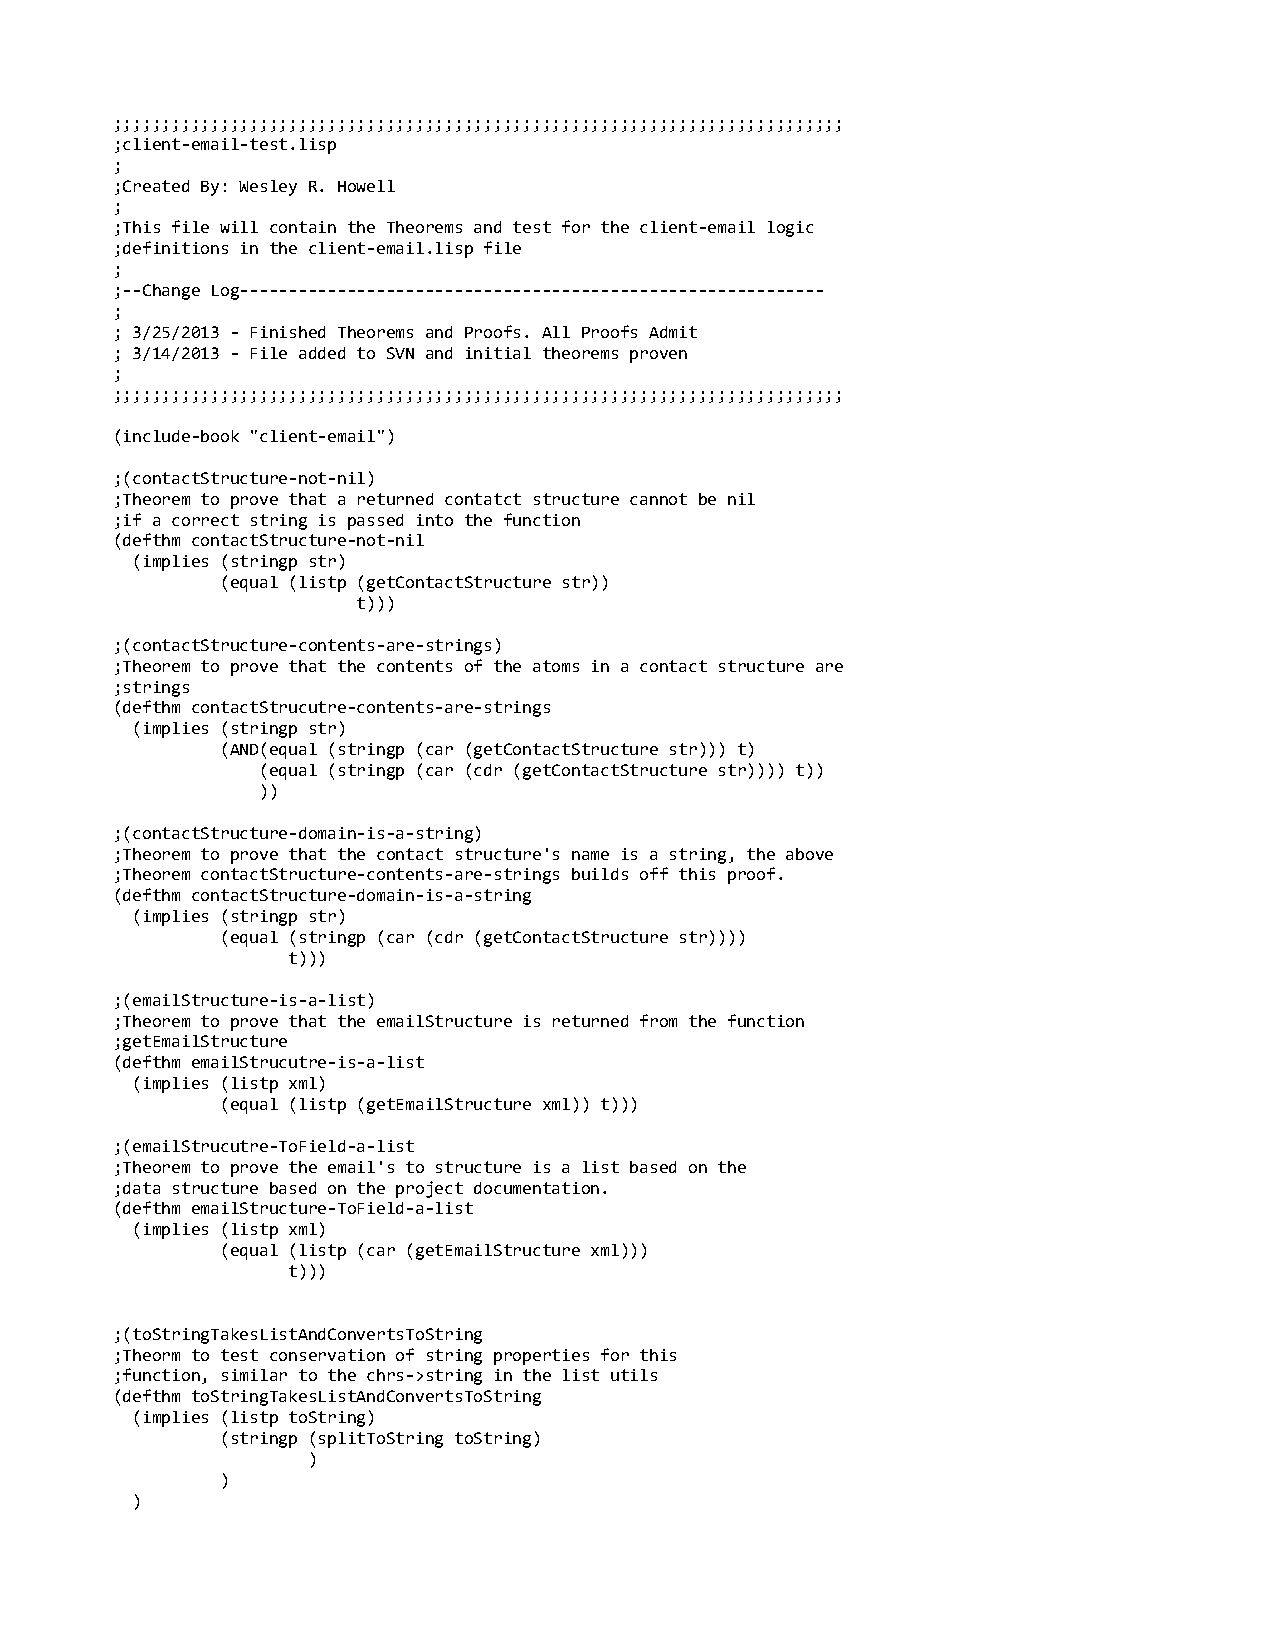
\includepdf[pages=1-3, pagecommand={}, scale=0.93]{clinet-email-test}

\item[\large Appendix C: Java Source Code Files]\hfill \\
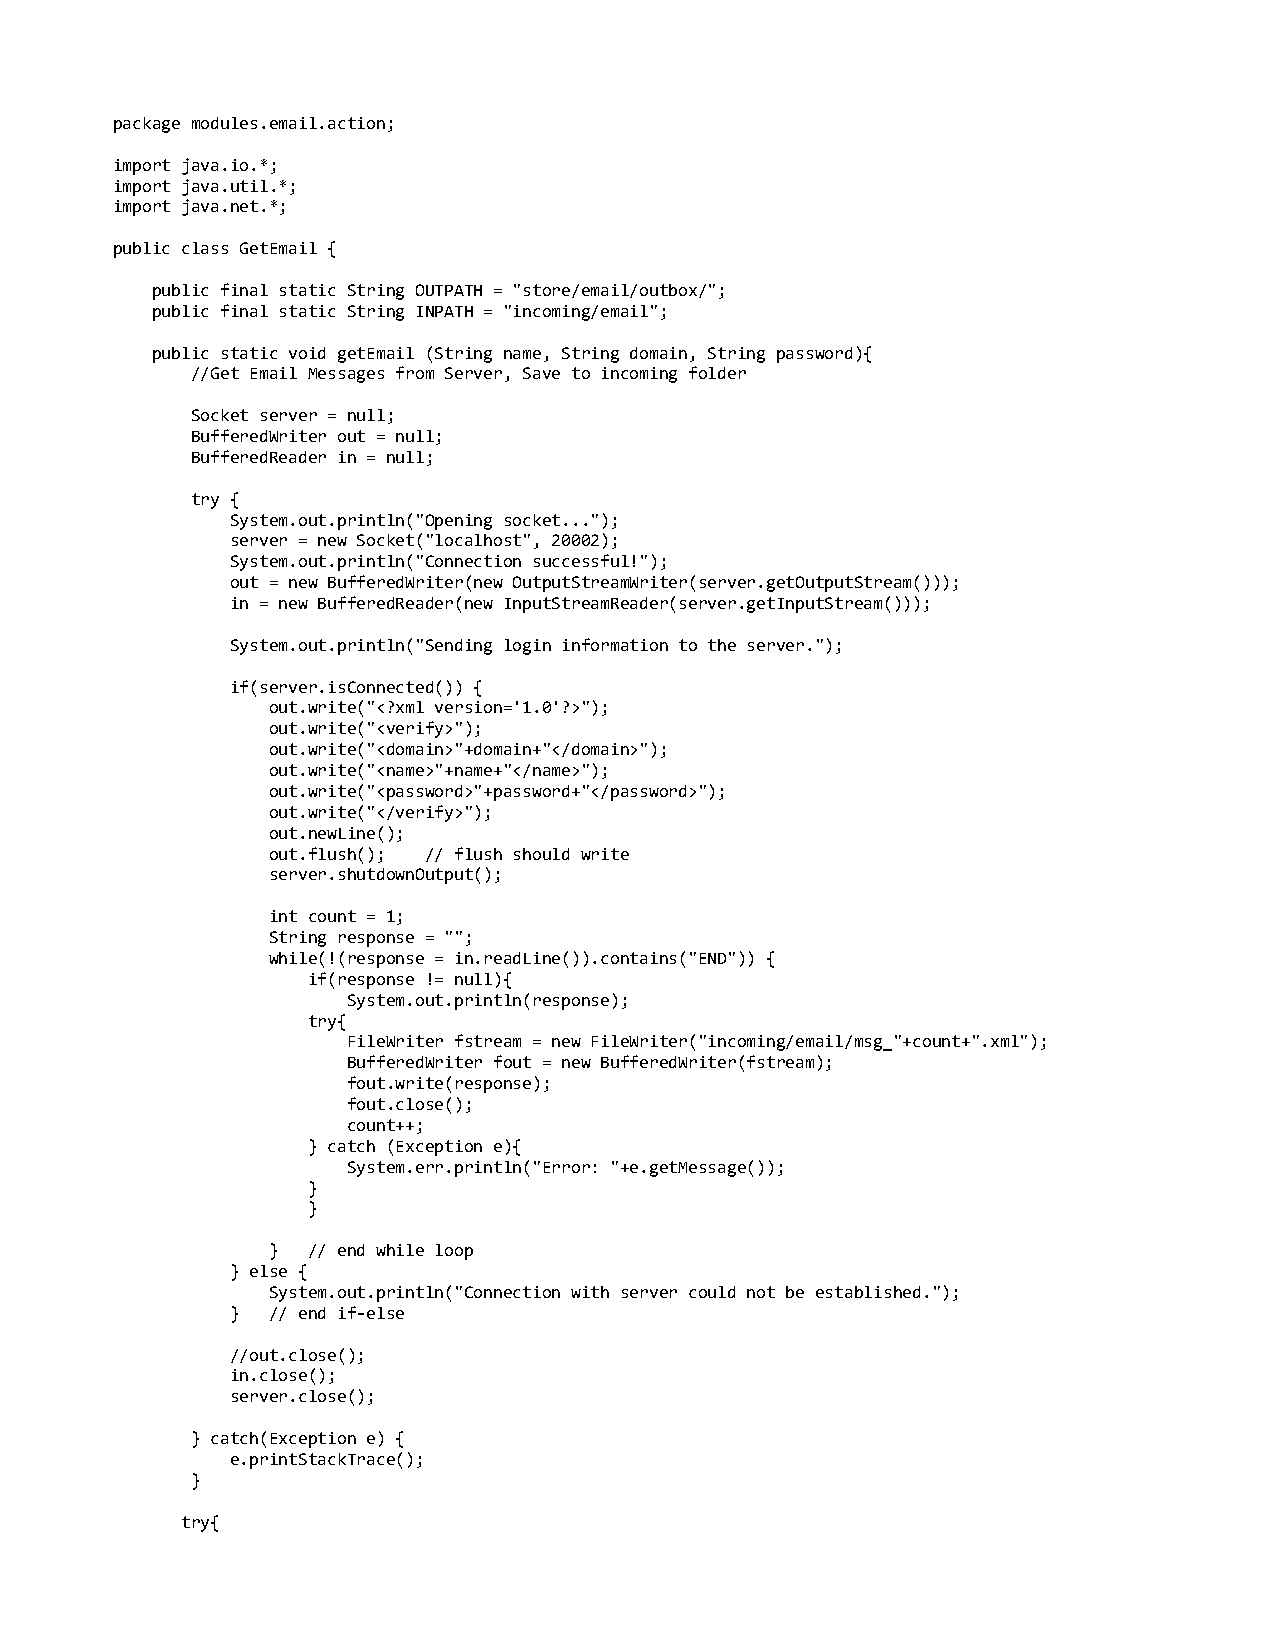
\includepdf[pages=1-2, pagecommand={}, scale=0.93]{GetEmail}
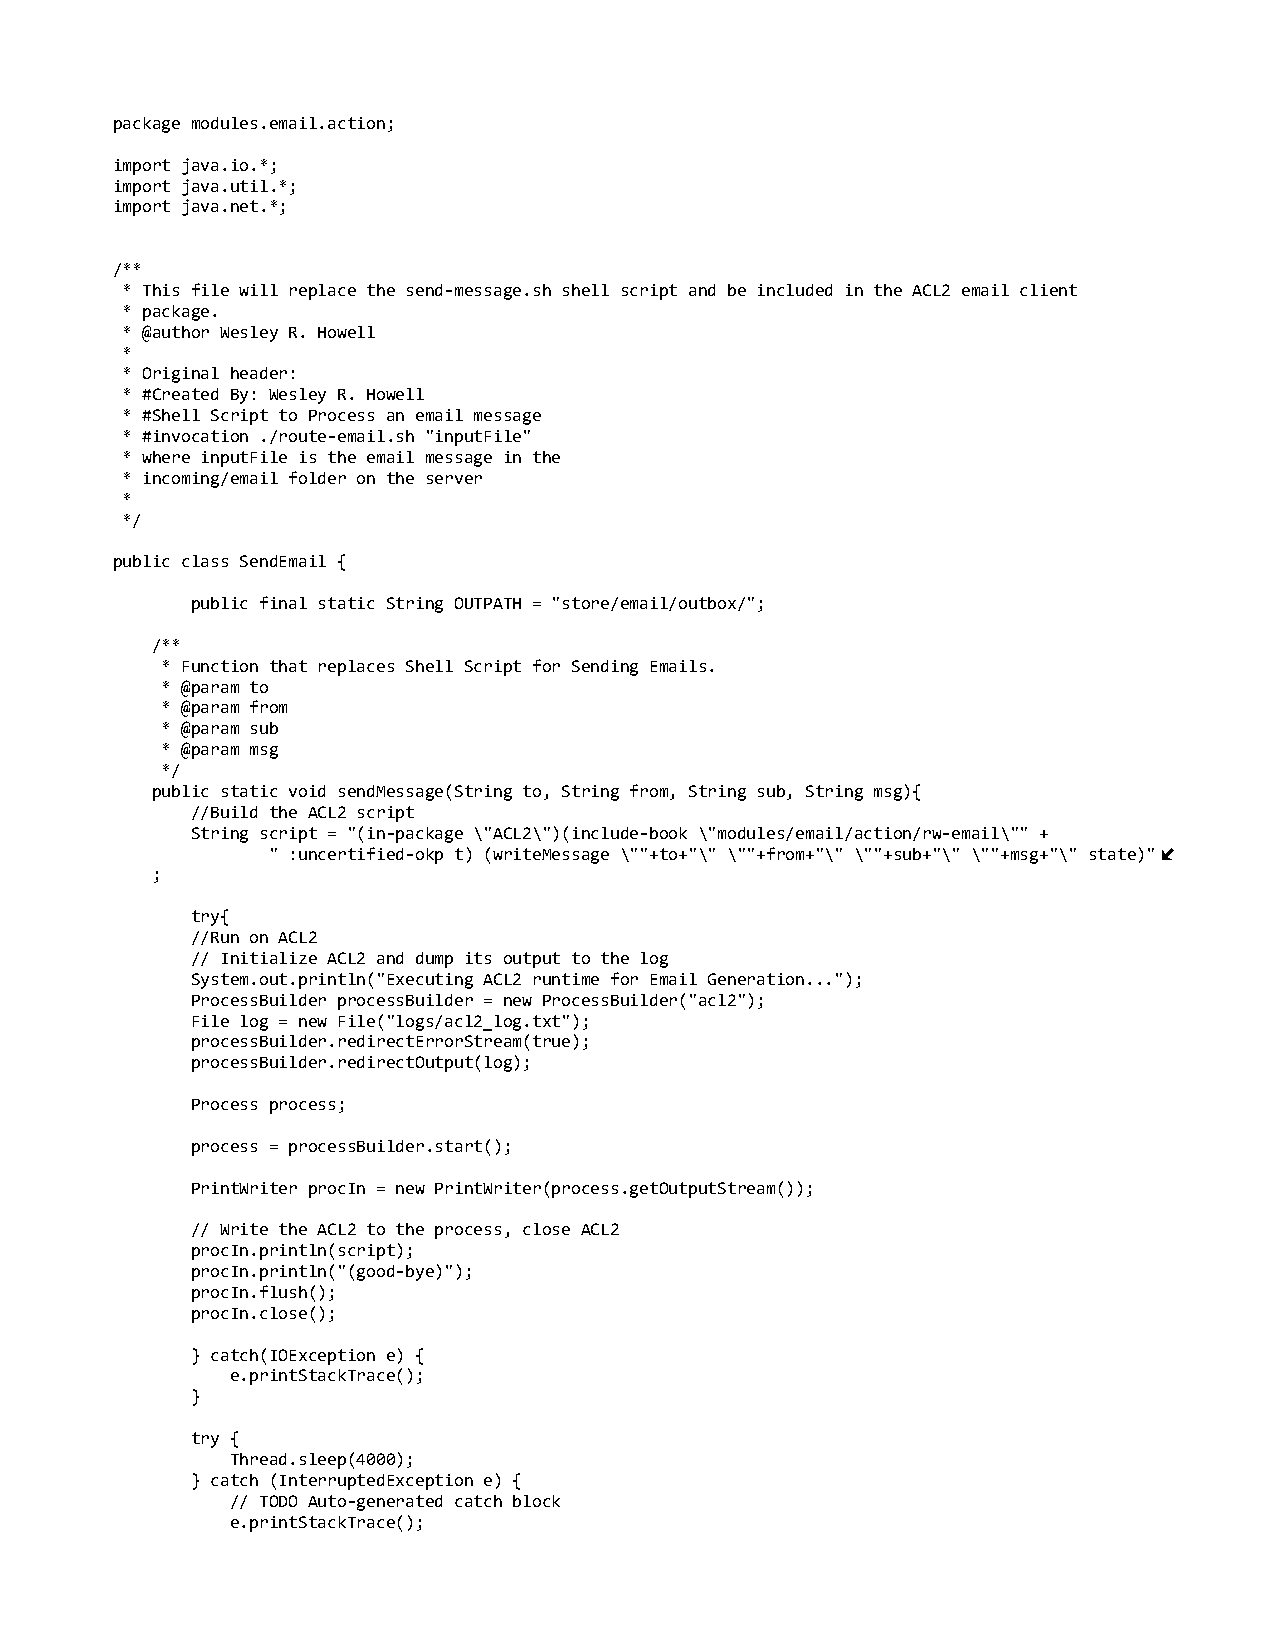
\includepdf[pages=1-3, pagecommand={}, scale=0.93]{SendEmail}
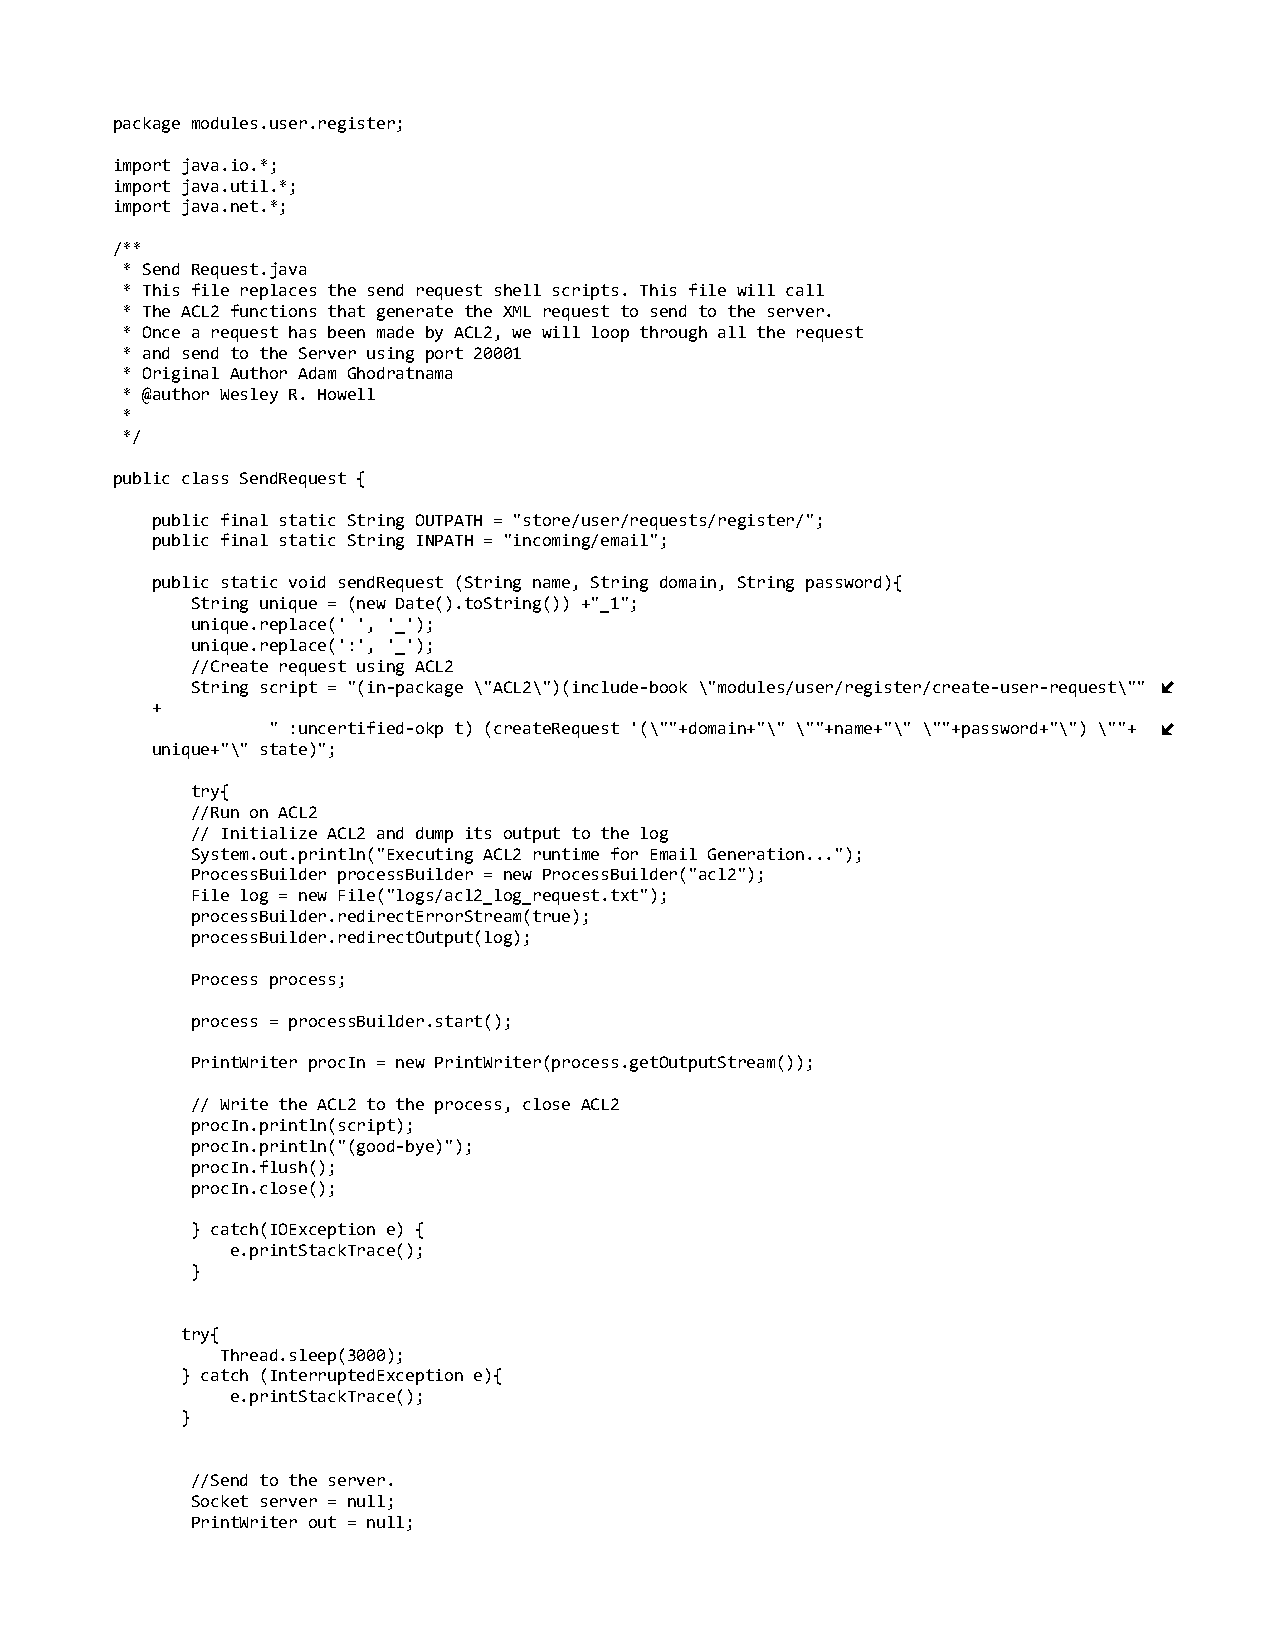
\includepdf[pages=1-2, pagecommand={}, scale=0.93]{SendRequest}

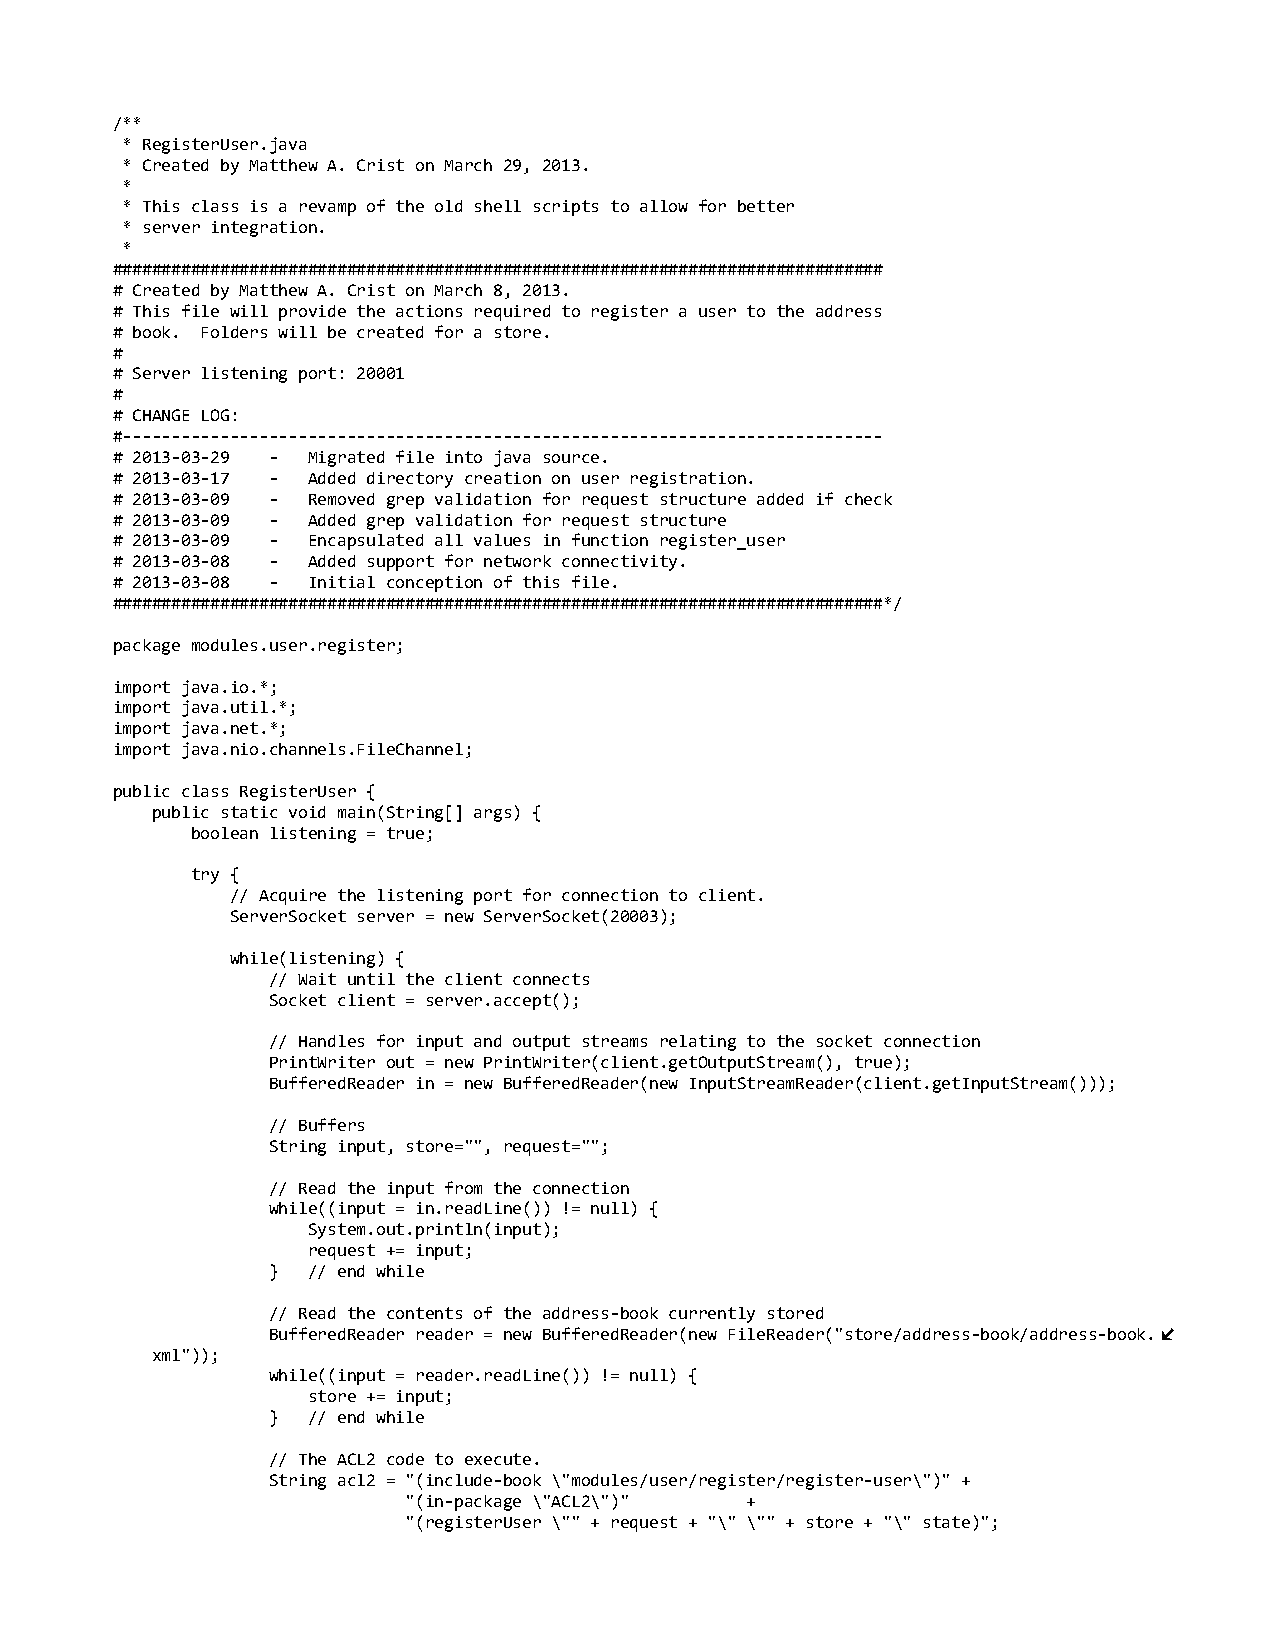
\includepdf[pages=1-3, pagecommand={}, scale=0.93]{RegisterUser}
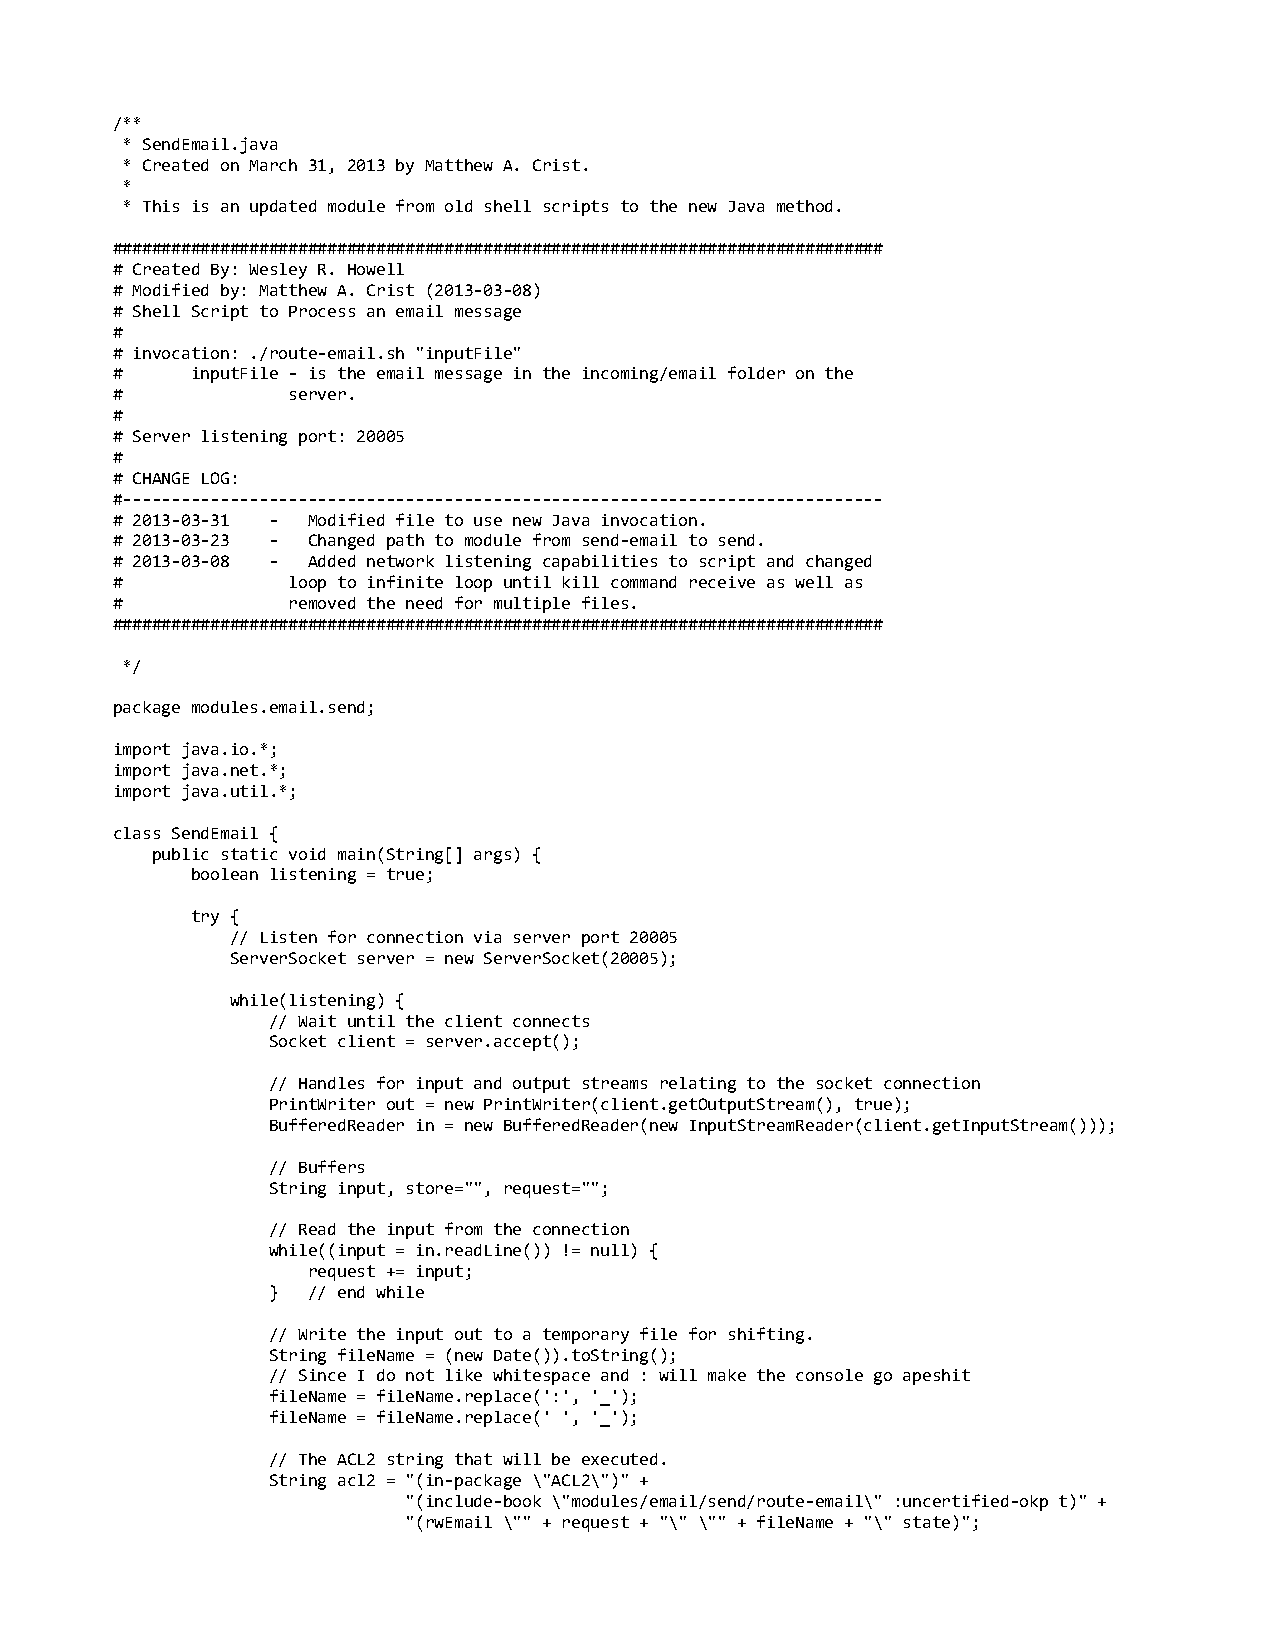
\includepdf[pages=1-2, pagecommand={}, scale=0.93]{SSendEmail}
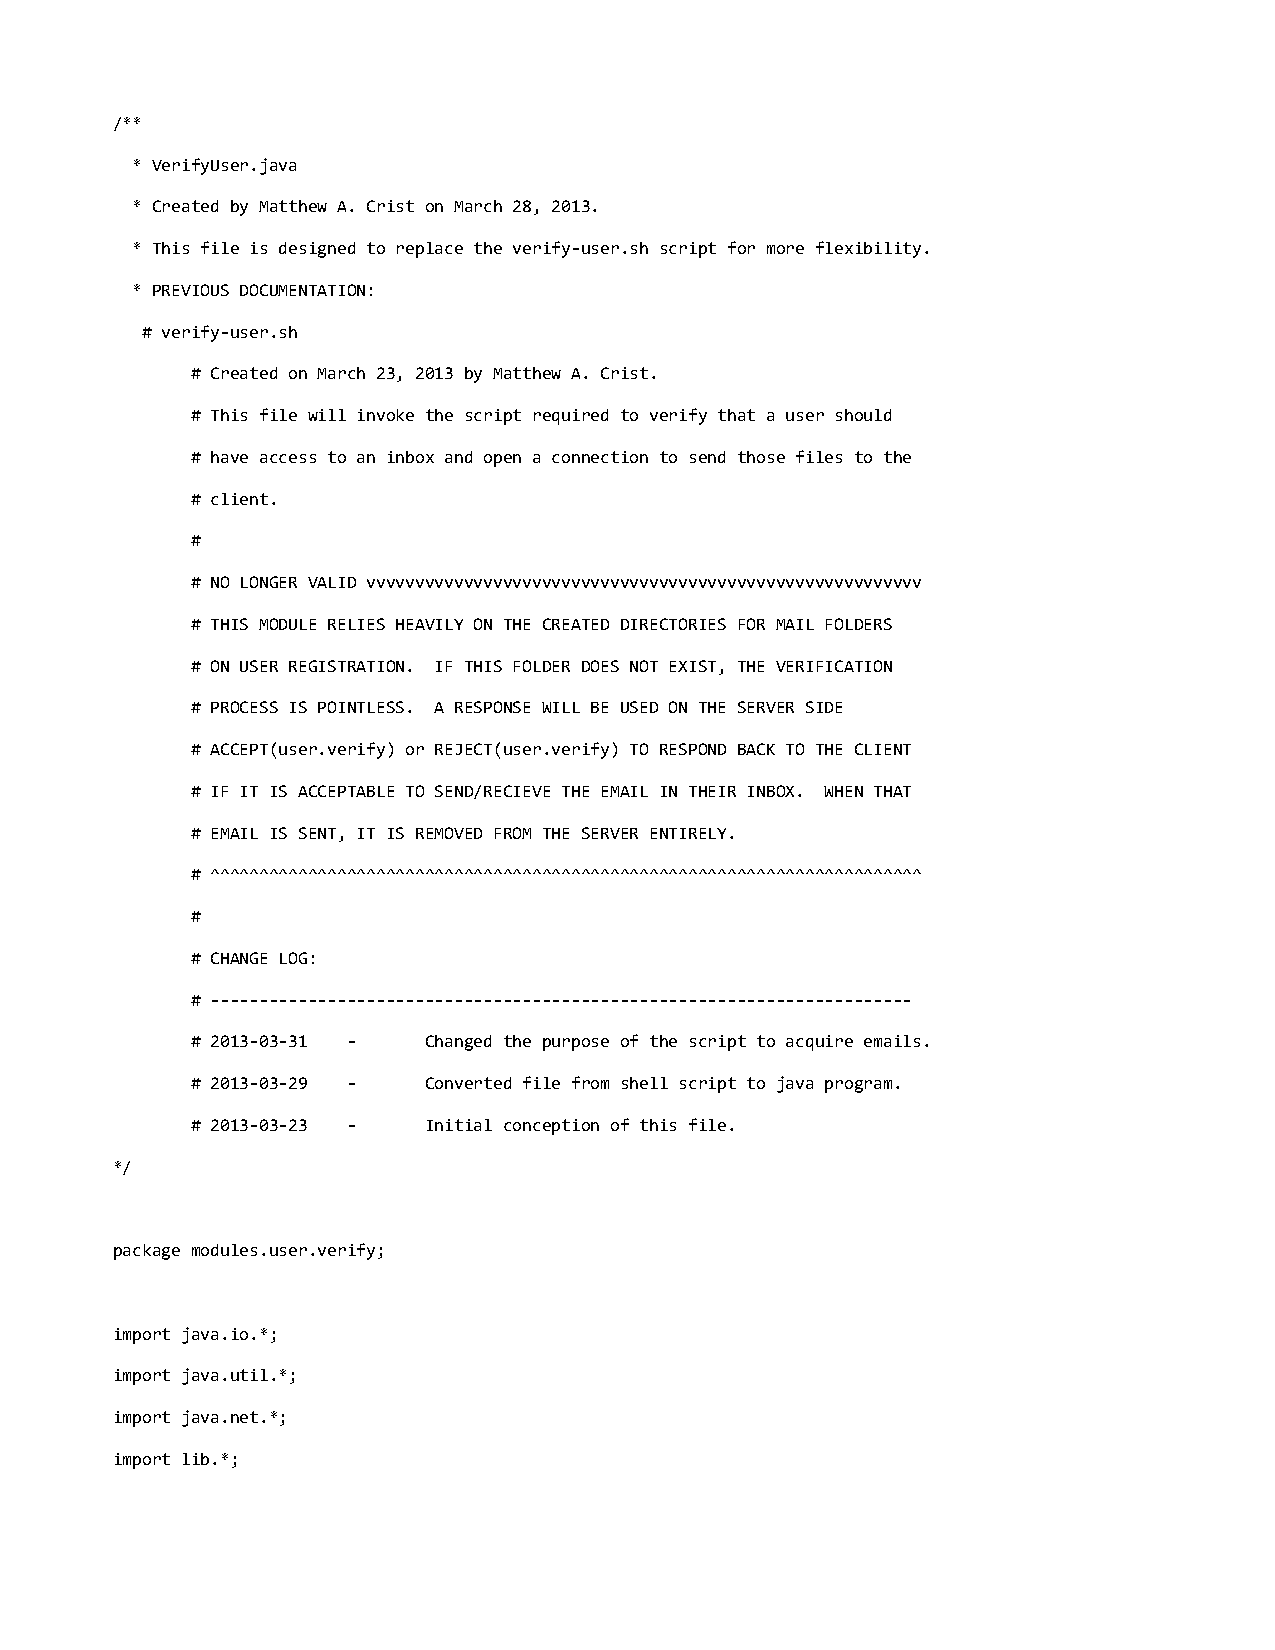
\includepdf[pages=1-6, pagecommand={}, scale=0.93]{VerifyUser}

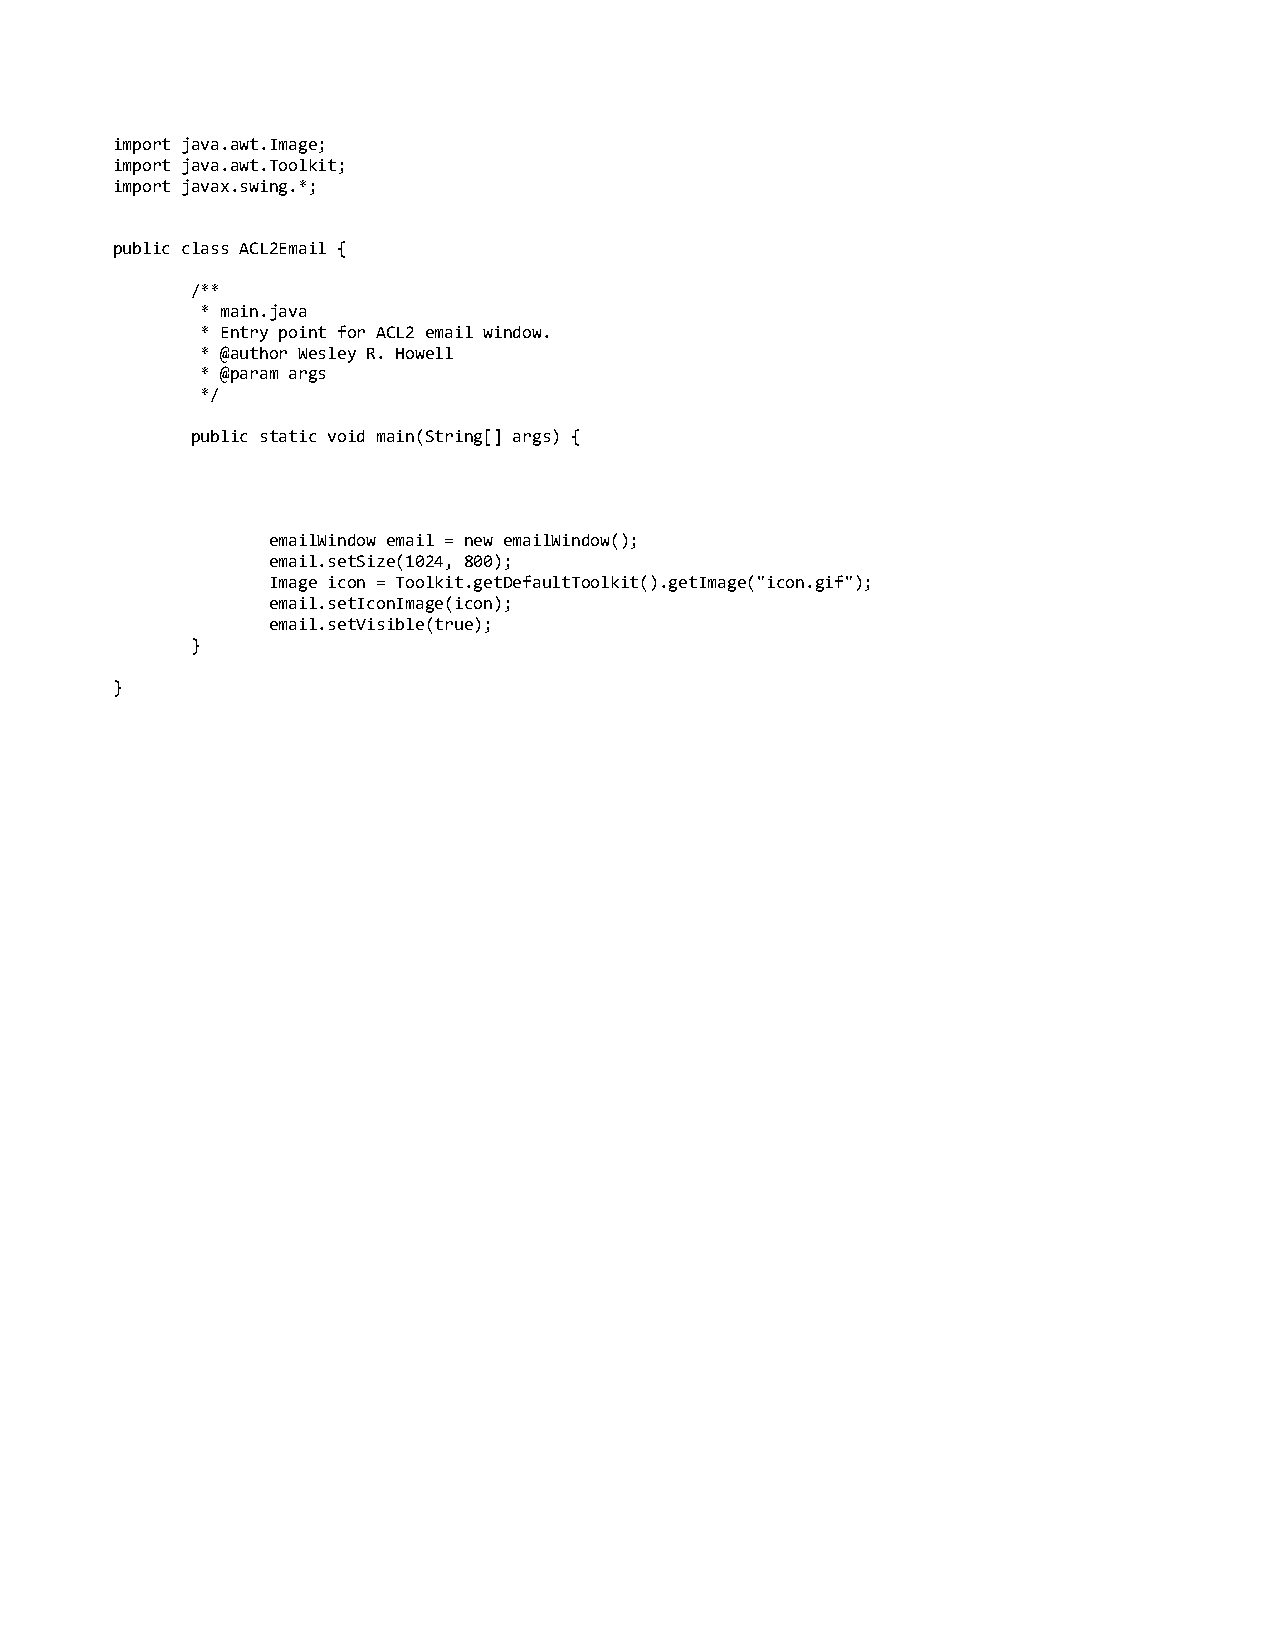
\includepdf[pages=1-1, pagecommand={}, scale=0.93]{ACL2Email}
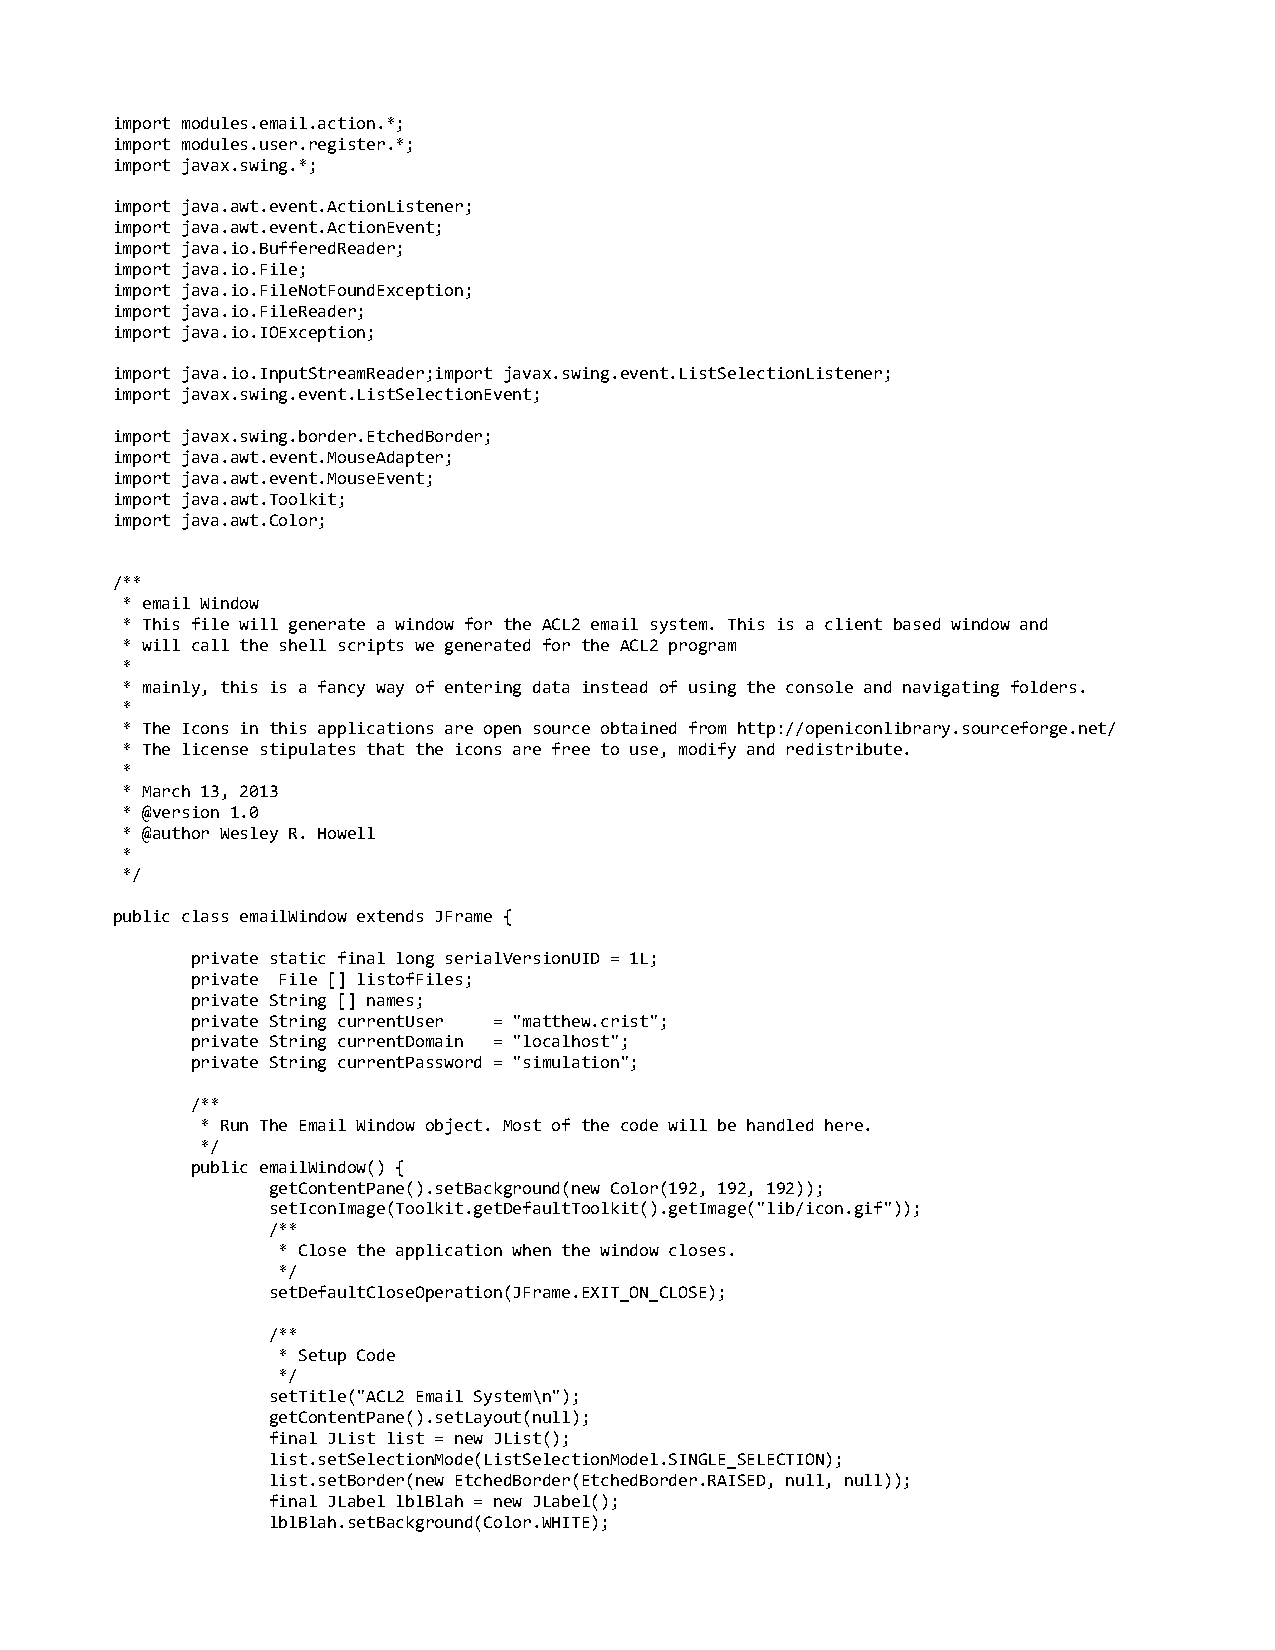
\includepdf[pages=1-6, pagecommand={}, scale=0.93]{emailWindow}
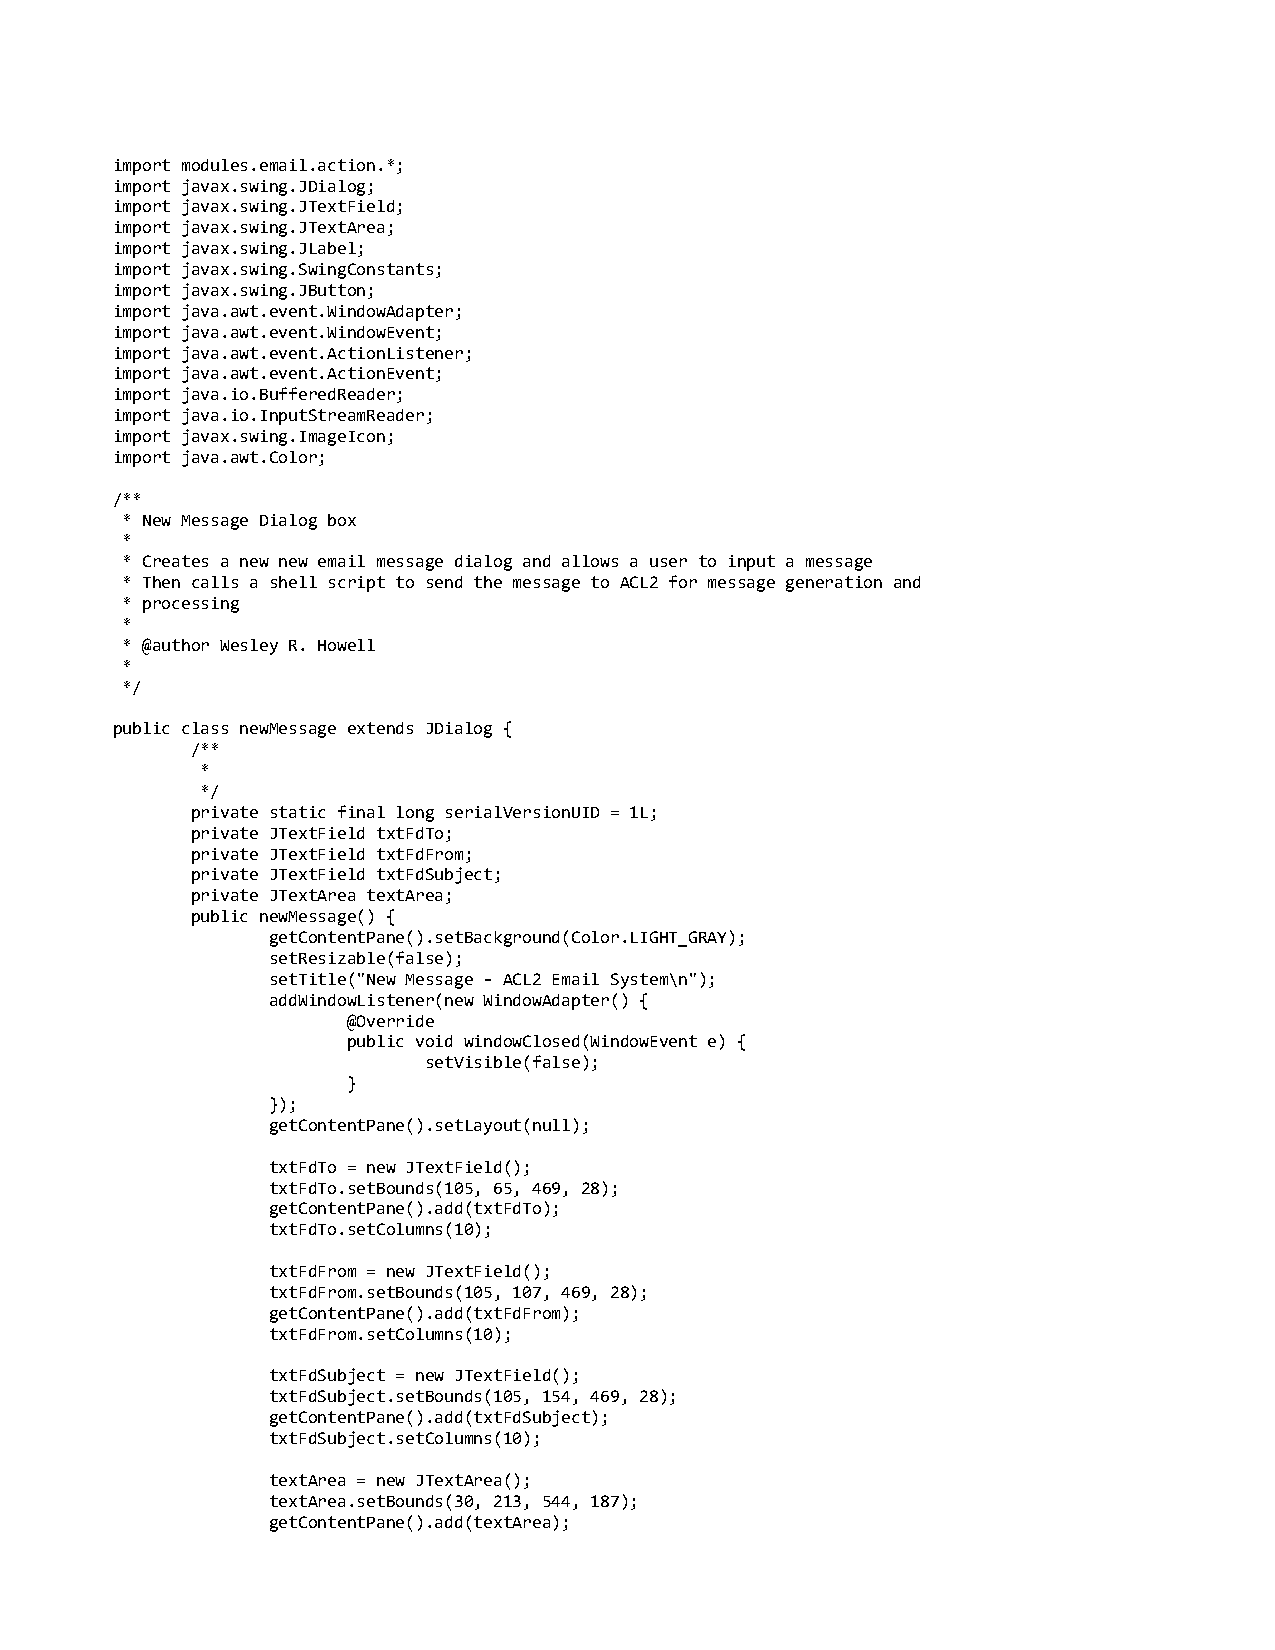
\includepdf[pages=1-3, pagecommand={}, scale=0.93]{newMessage}

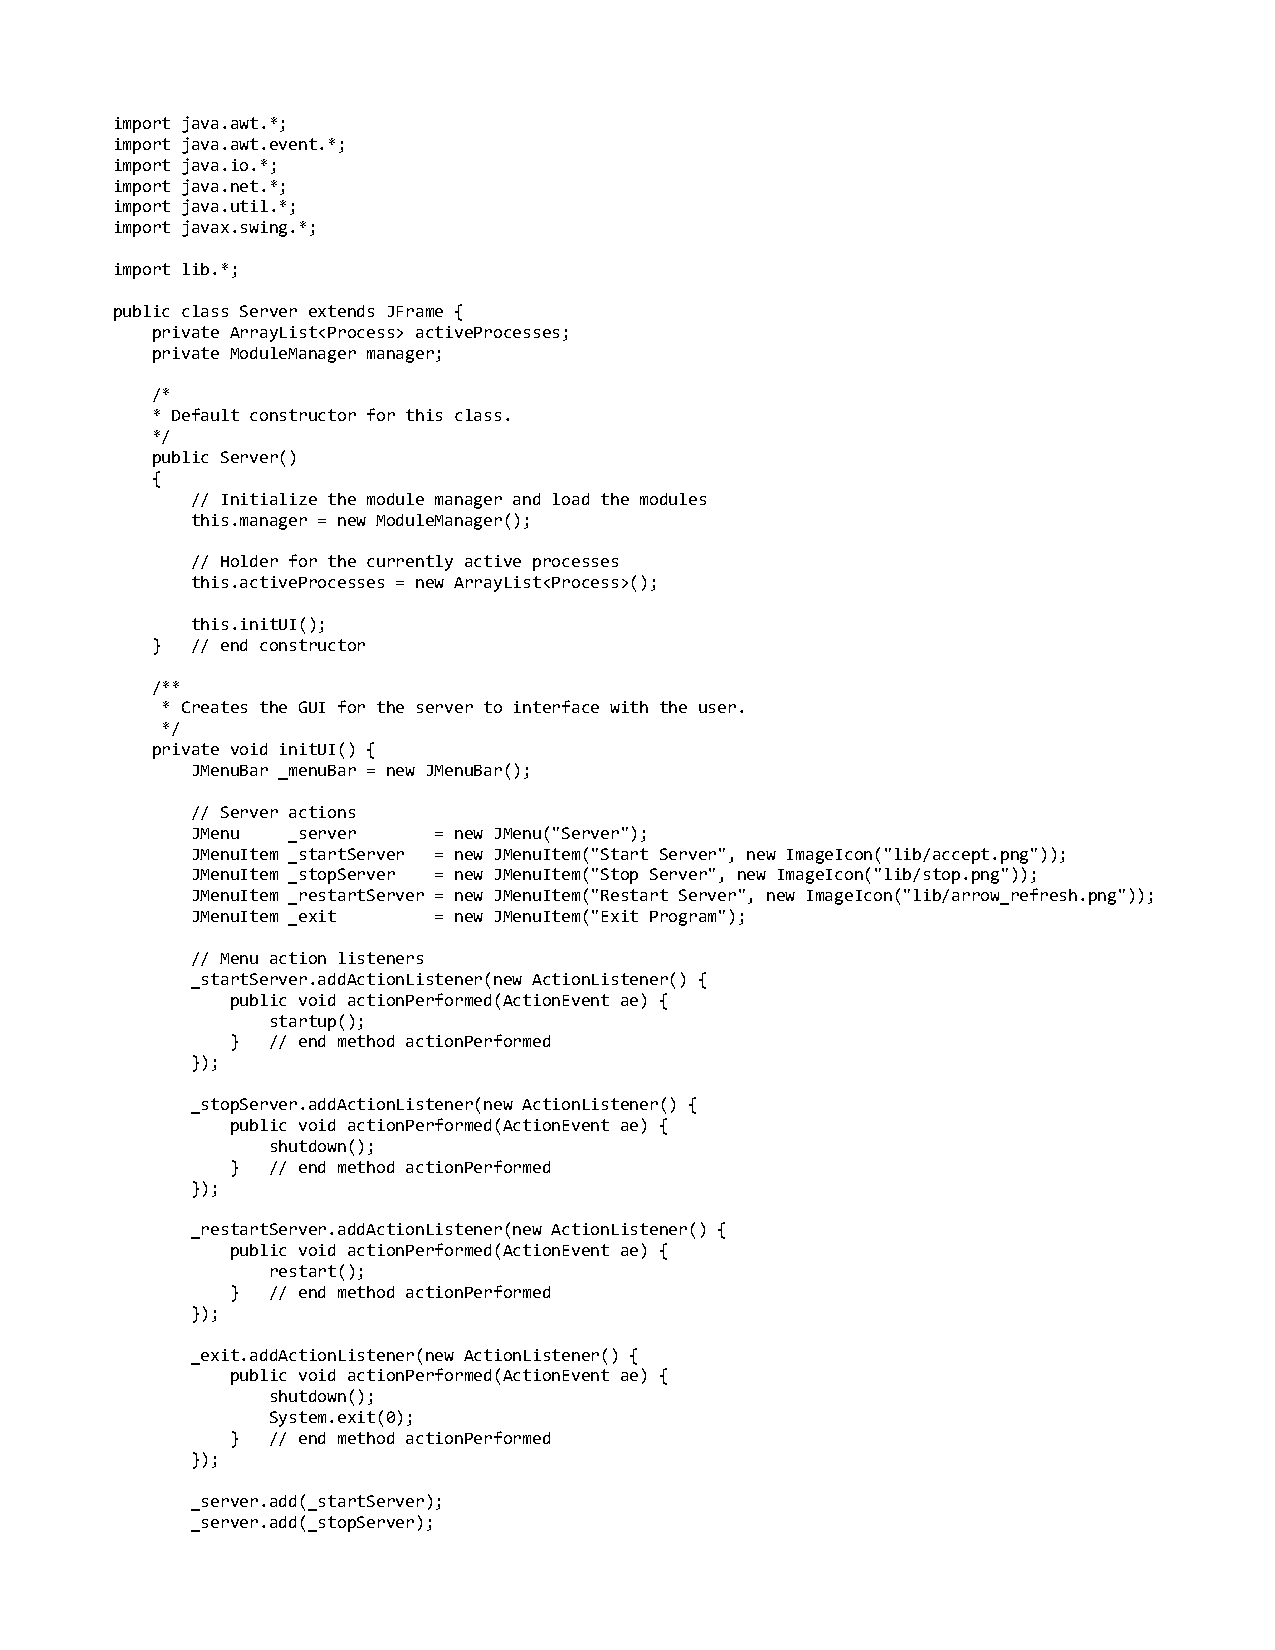
\includepdf[pages=1-3, pagecommand={}, scale=0.93]{Server}
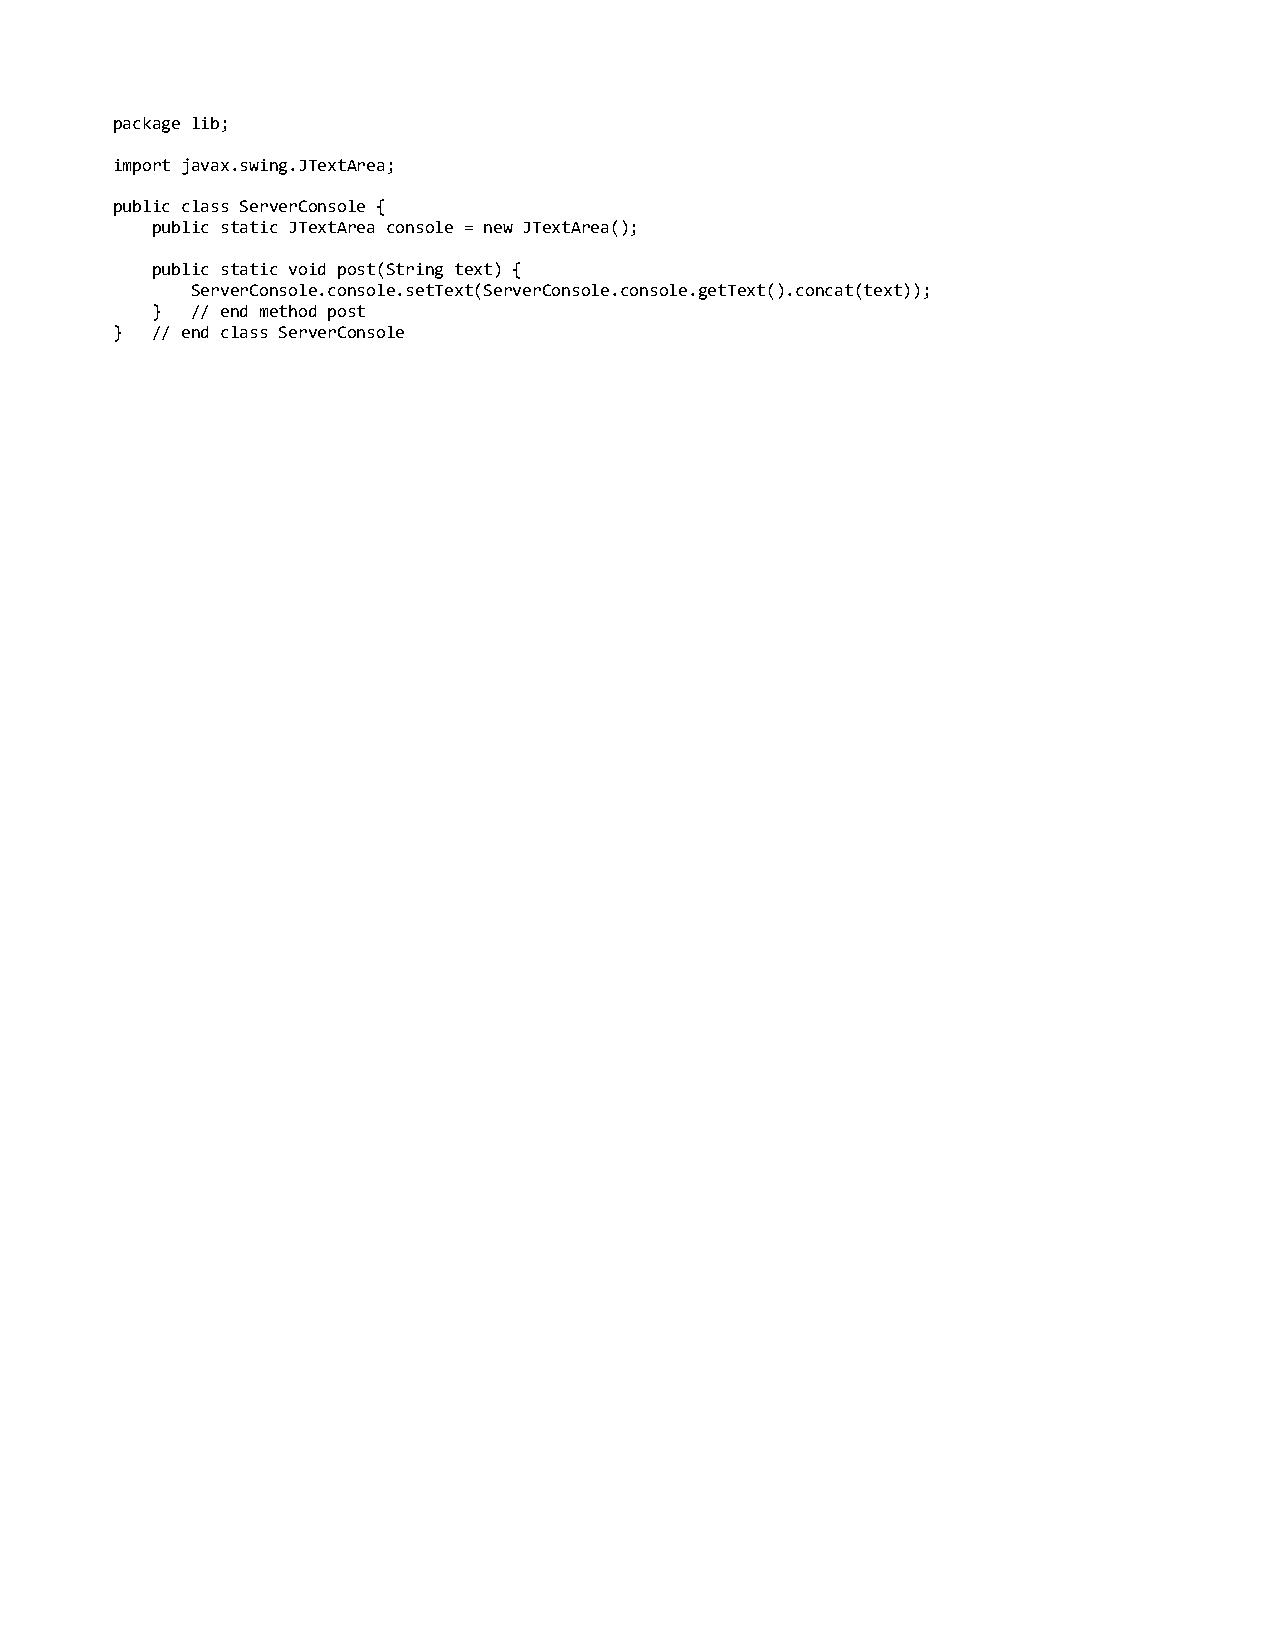
\includepdf[pages=1-1, pagecommand={}, scale=0.93]{ServerConsole}
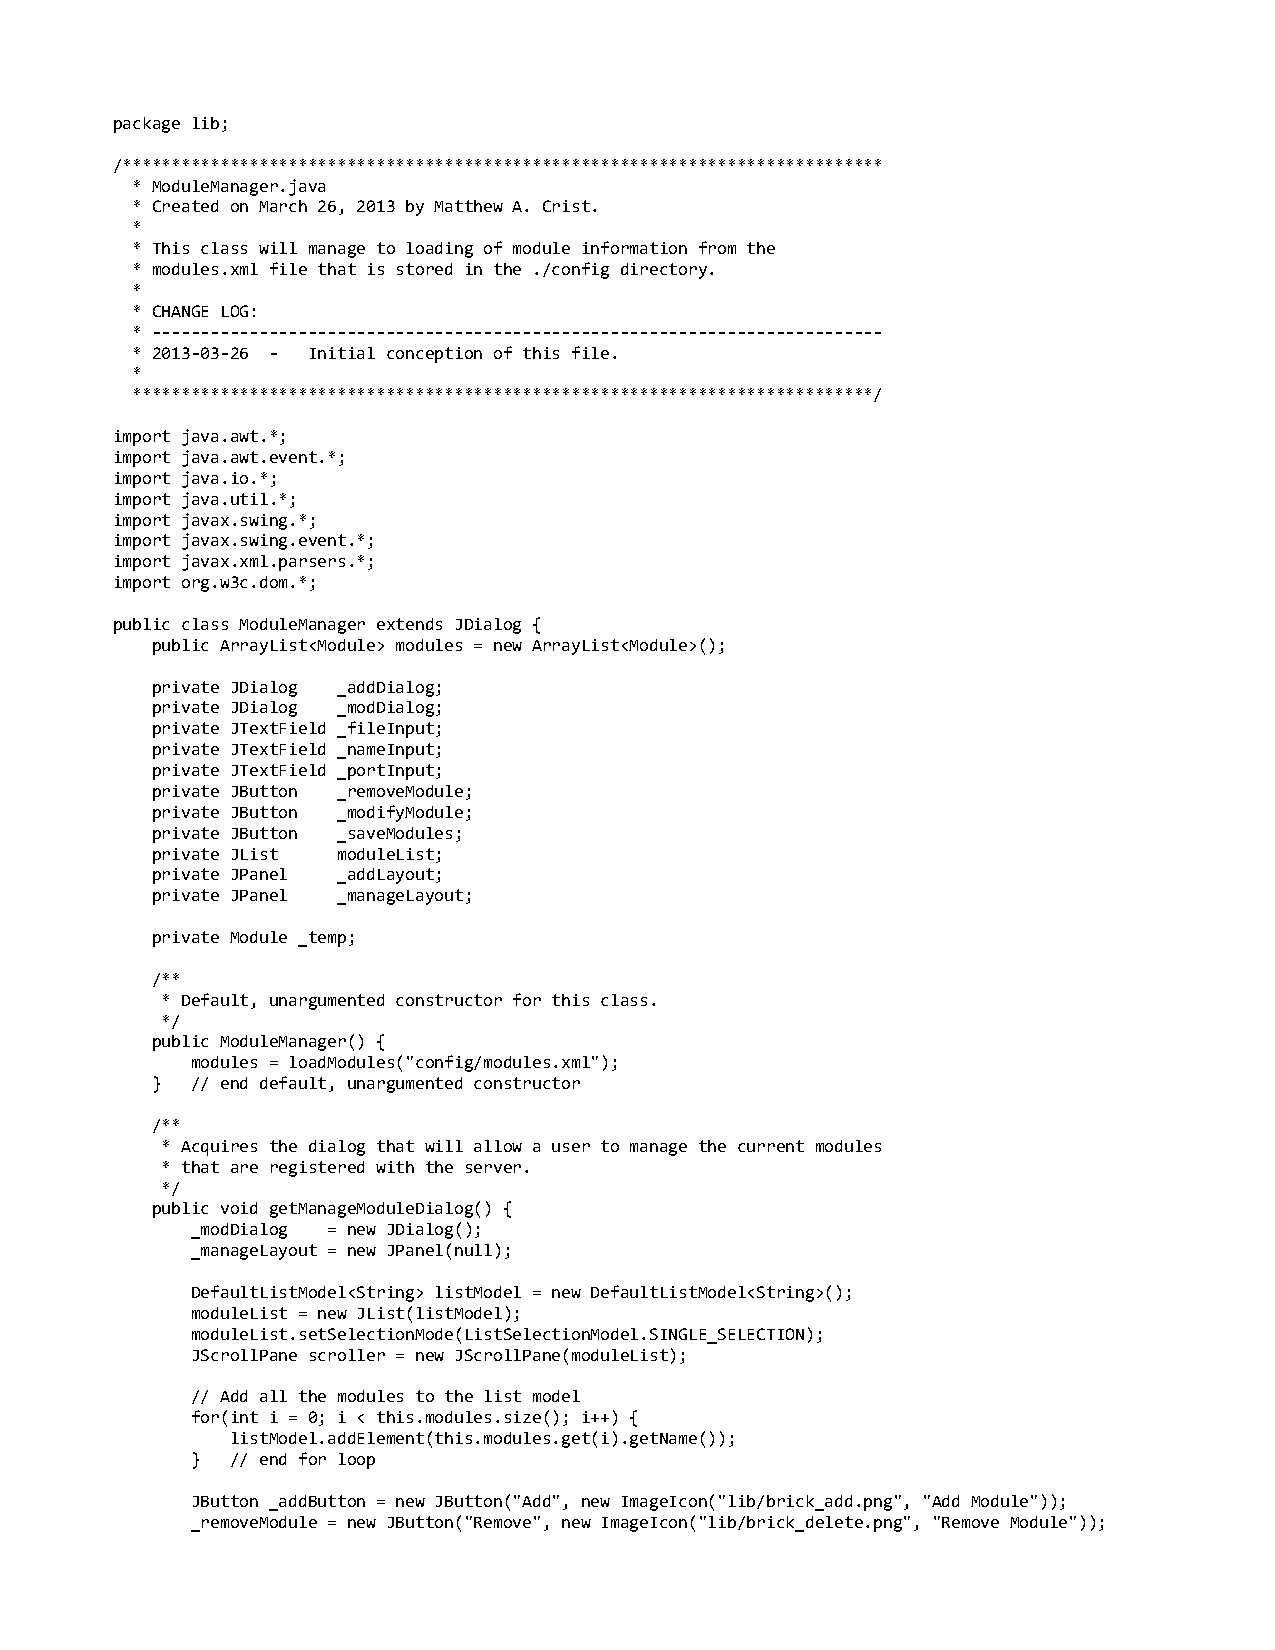
\includepdf[pages=1-7, pagecommand={}, scale=0.93]{ModuleManager}
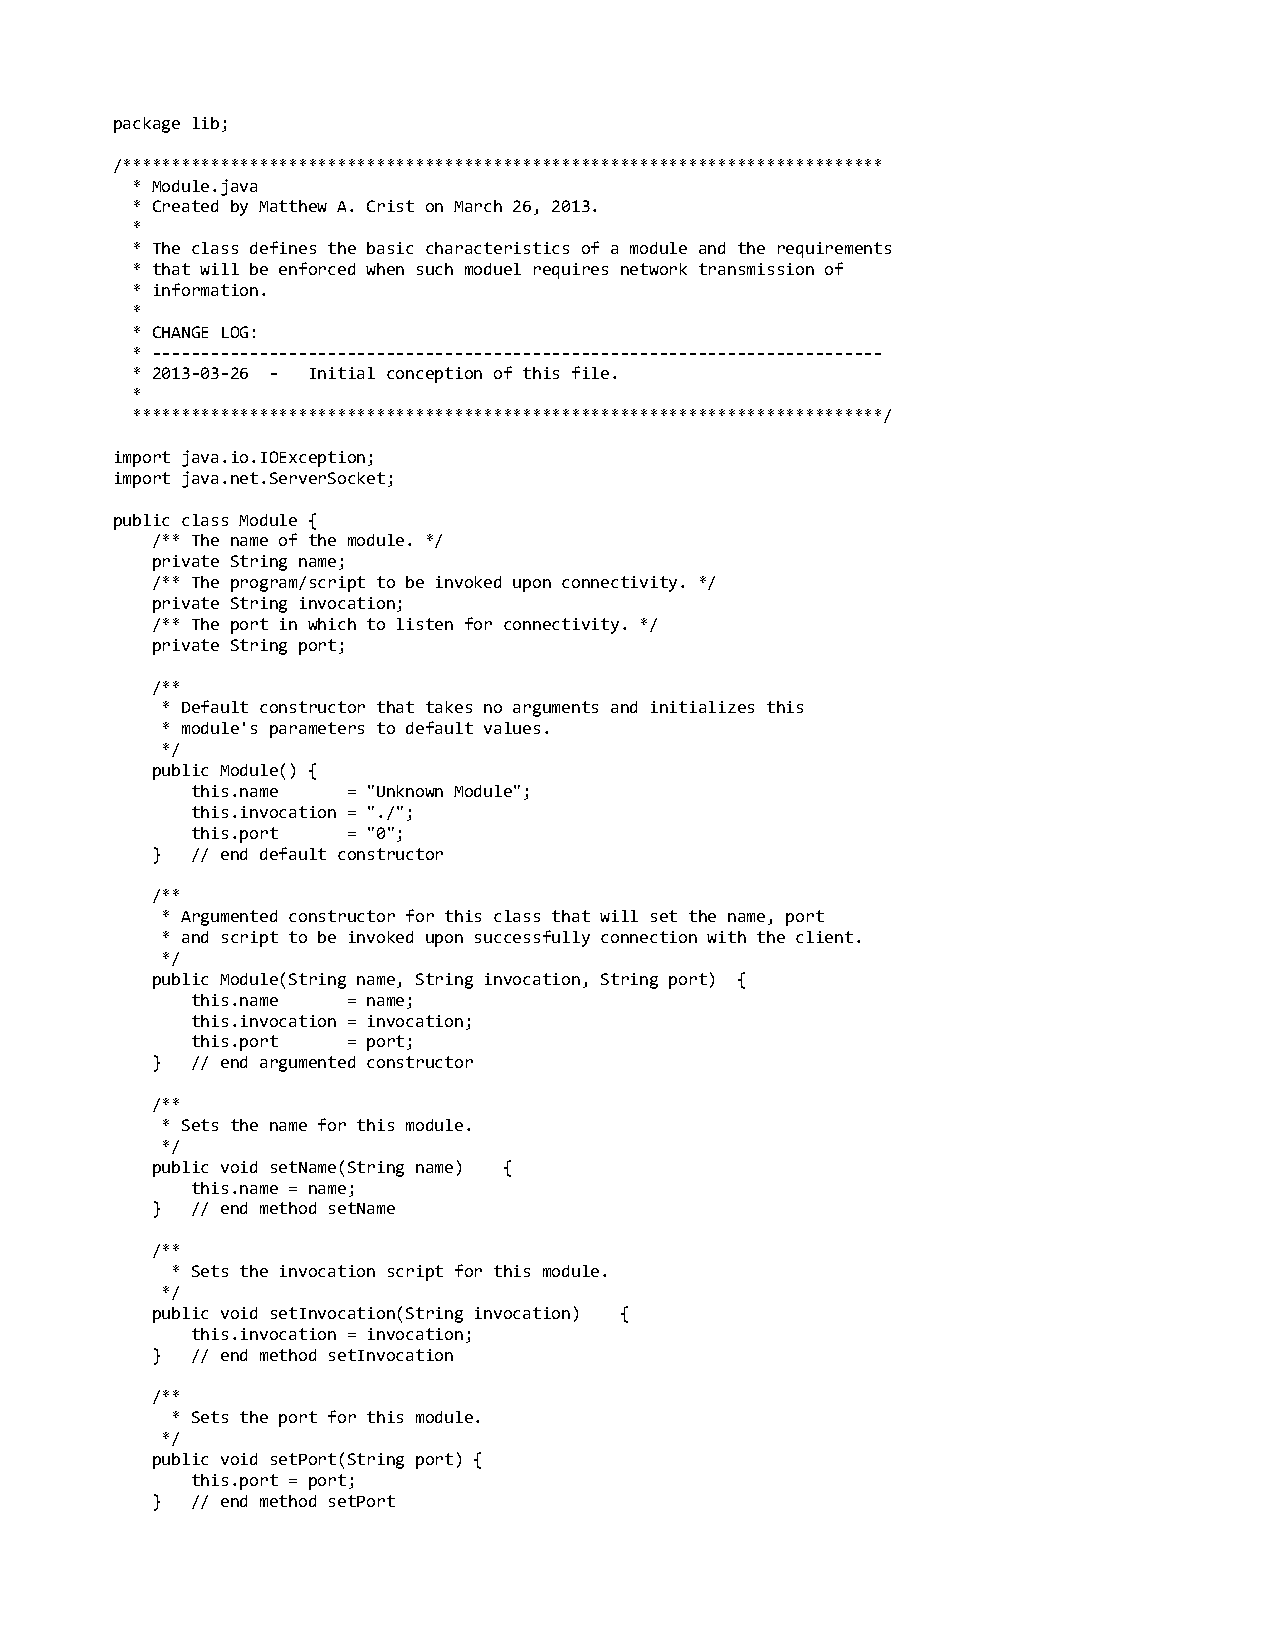
\includepdf[pages=1-2, pagecommand={}, scale=0.93]{Module}


\newpage 
\item [\large Appendix D: PSP File for Main Project]\hfill
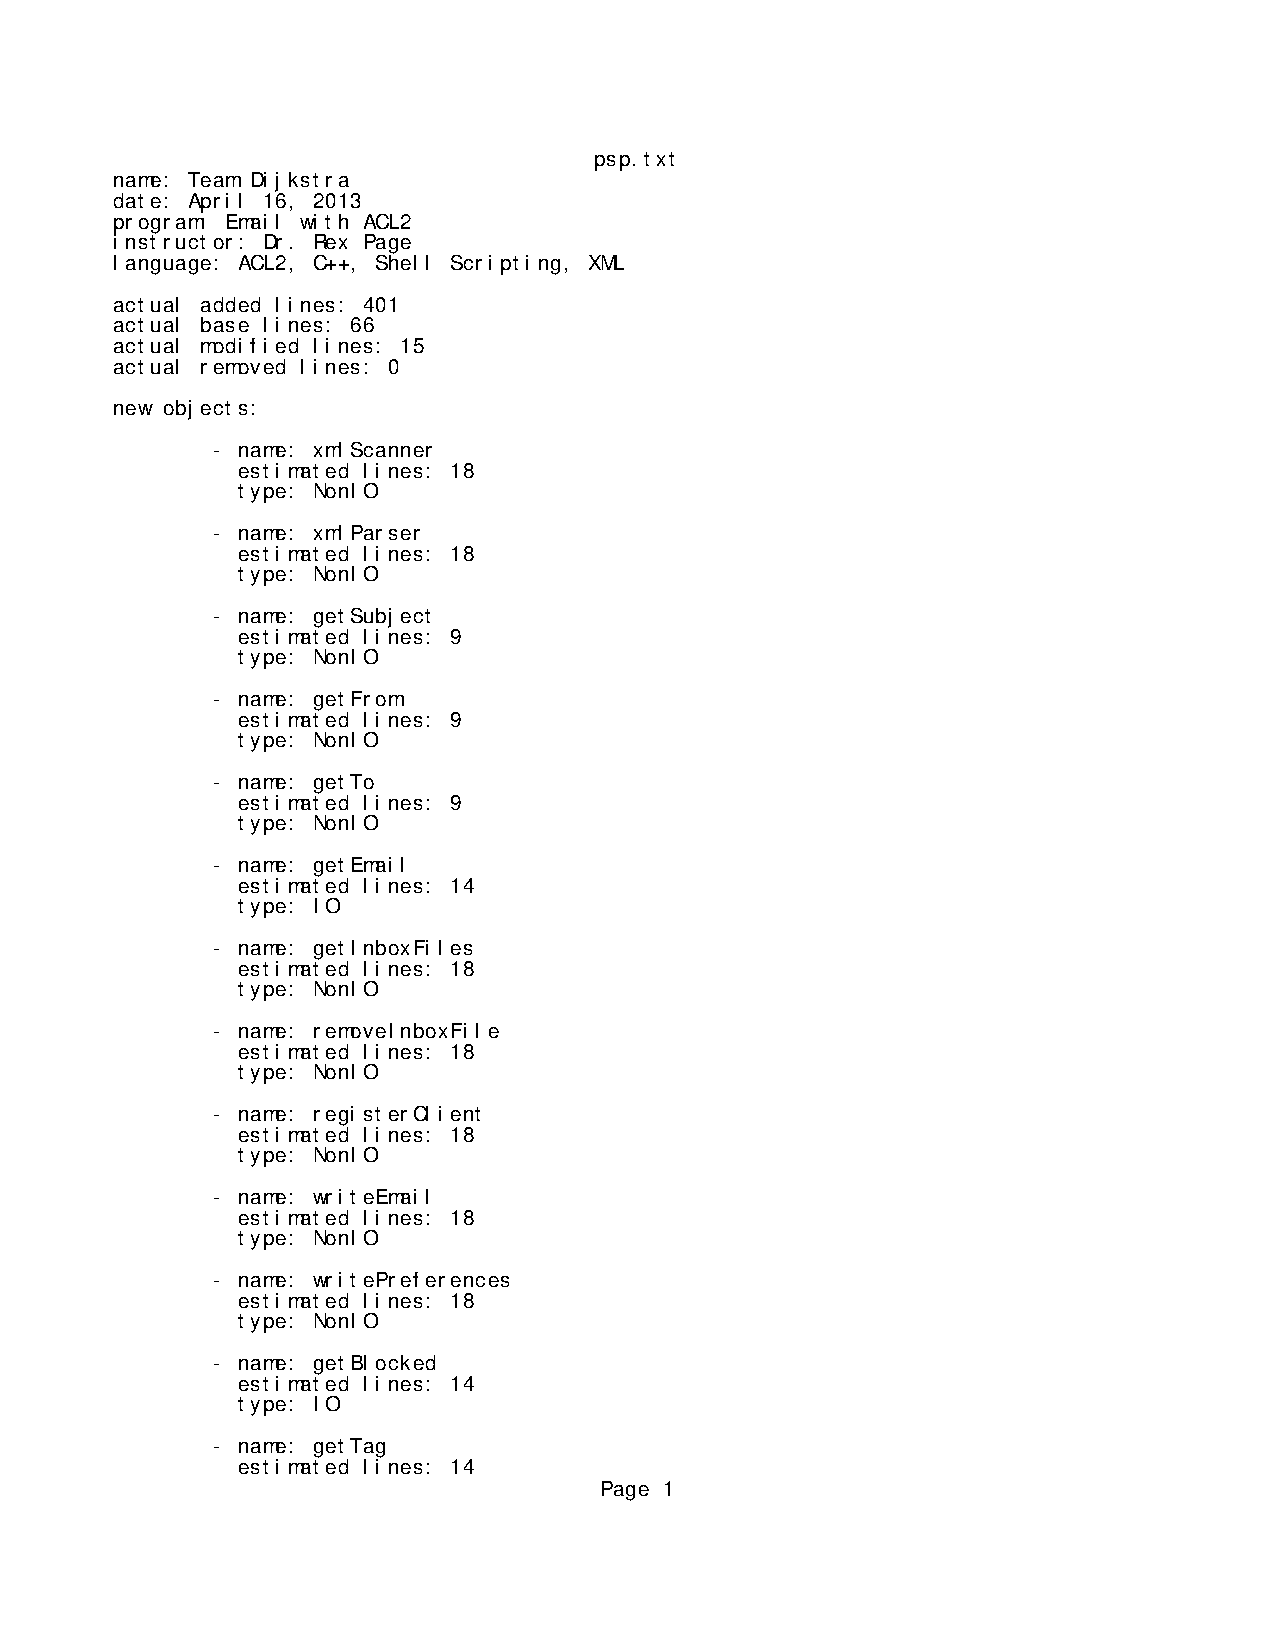
\includepdf[pages=1-22, pagecommand={}, scale=0.93]{psp}


\newpage
\item[\large Appendix D: PSP File for Additional Features PROBE Estimate] \hfill
\begin{verbatim}
name: Team Dijkstra
date: January 31, 2013
program: Additional Features
instructor: Dr. Rex Page
language: ACL2



new objects:

	- name: isSecureMessage
	  estimated lines: 6
	  type: NonIO

	- name: postToSecureClient
	  estimated lines: 16
	  type: I/O

	- name: getSecureMessages
	  estimated lines: 16
	  type: I/O

	- name: getSecurityCredential
	  estimated lines: 9
	  type: NonIO

	- name: authorizeSecureClient
	  estimated lines: 9
	  type: NonIO

	- name: registerSecureClient
	  estimated lines: 9
	  type: NonIO

	- name: isSecuredMessage
	  estimated lines: 9
	  type: NonIO

	- name: setSecuredType
	  estimated lines: 14
	  type: IO

	- name: getSecuredOutput
	  estimated lines: 18
	  type: NonIO

	- name: postSecuredMessage
	  estimated lines: 16
	  type: IO

	- name: inputEncryptionCode
	  estimated lines: 9
	  type: NonIO

	- name: encryptMessage
	  estimated lines: 9
	  type: NonIO

	- name: decryptMessage
	  estimated lines: 9
	  type: NonIO

	- name: openAttachmentFile
	  estimated lines: 16
	  type: IO

	- name: attachmentToBytes
	  estimated lines: 18
	  type: NonIO

	- name: attachmentToXML
	  estimated lines: 18
	  type: NonIO

	- name: addToBody
	  estimated lines: 9
	  type: NonIO

	- name: encryptAttachment
	  estimated lines: 18
	  type: NonIO

	- name: decryptAttachment
	  estimated lines: 18
	  type: NonIO

	- name: xmlReaderForAttachments
	  estimated lines: 18
	  type: NonIO

	- name: sendAttachmentToServer
	  estimated lines: 16
	  type: IO

	- name: getAttachmentsFromServer
	  estimated lines: 14
	  type: IO

	- name: setAttachmentKey
	  estimated lines: 9
	  type: NonIO
\end{verbatim}

\newpage
\item[\large Appendix E: Engineering Procedures and Standards] 
\hypertarget{Overview} {}
\item[Overview] \hfill \\ 
The purpose of this document is to define the engineering standards and procedures for Team Dijkstra's Software Engineering II project. \\ \\
This document will contain information regarding our Source Code Control, Defect Database Design, Coding Style Sheet, Rationale for Language Choice, and updated PROBE Table. \\ \\
This document will serve as a team reference guide when it comes to actual implementation of the project. This will help keep solidify and help keep our code design and style uniform. \\

\hypertarget{Source} {}
\item[Source-Code Control] \hfill \\ 
To control and maintain our source-code, our group is using Google Code's svn repository. Revision tracking and version control is centralized, and collaboration is simple. Each user has a Google account with which he can checkout the code. Anytime changes are made, svn keeps track and notes it in the repository. Only registered members of the group can upload changes to the repository as a security measure. \\

\hypertarget{DD} {}
\item[Defect Database Design] \hfill \\
Each defect will be reported using Google Code's Issues tracker. Each report will consist of the discoverer, a summary, the date, a description of the steps to reproduce the problem, a description of the error, and priority level. Once the issue is added to the database, anyone can read the defect report, work on fixing it, and update the status. \\ \\
In the defect database, the columns are labeled as follows: ID, Type, Status, Priority, Milestone, Owner, and Summary + Labels. After an issue has been resolved, it will move from being an open issue to a closed issue. The fixed issue will remain in the record for logging purposes.
When reporting, there are different labels that users can use to help categorize and organize the defects. First is the type of report. An issue can be a "defect," which is a report of a software defect, or it can be an "enhancement," which is a suggestion for software improvement. There can also be a "review," which is a request for a source code review. The second type of label is the priority level. Priority critical is an issue that must be resolved in order for the project to be functional. Priority high is an issue that is strongly wanted. Priority medium is a normal bug. Priority low is an issue that can be resolved eventually. 

\newpage
\hypertarget{CSS} {}

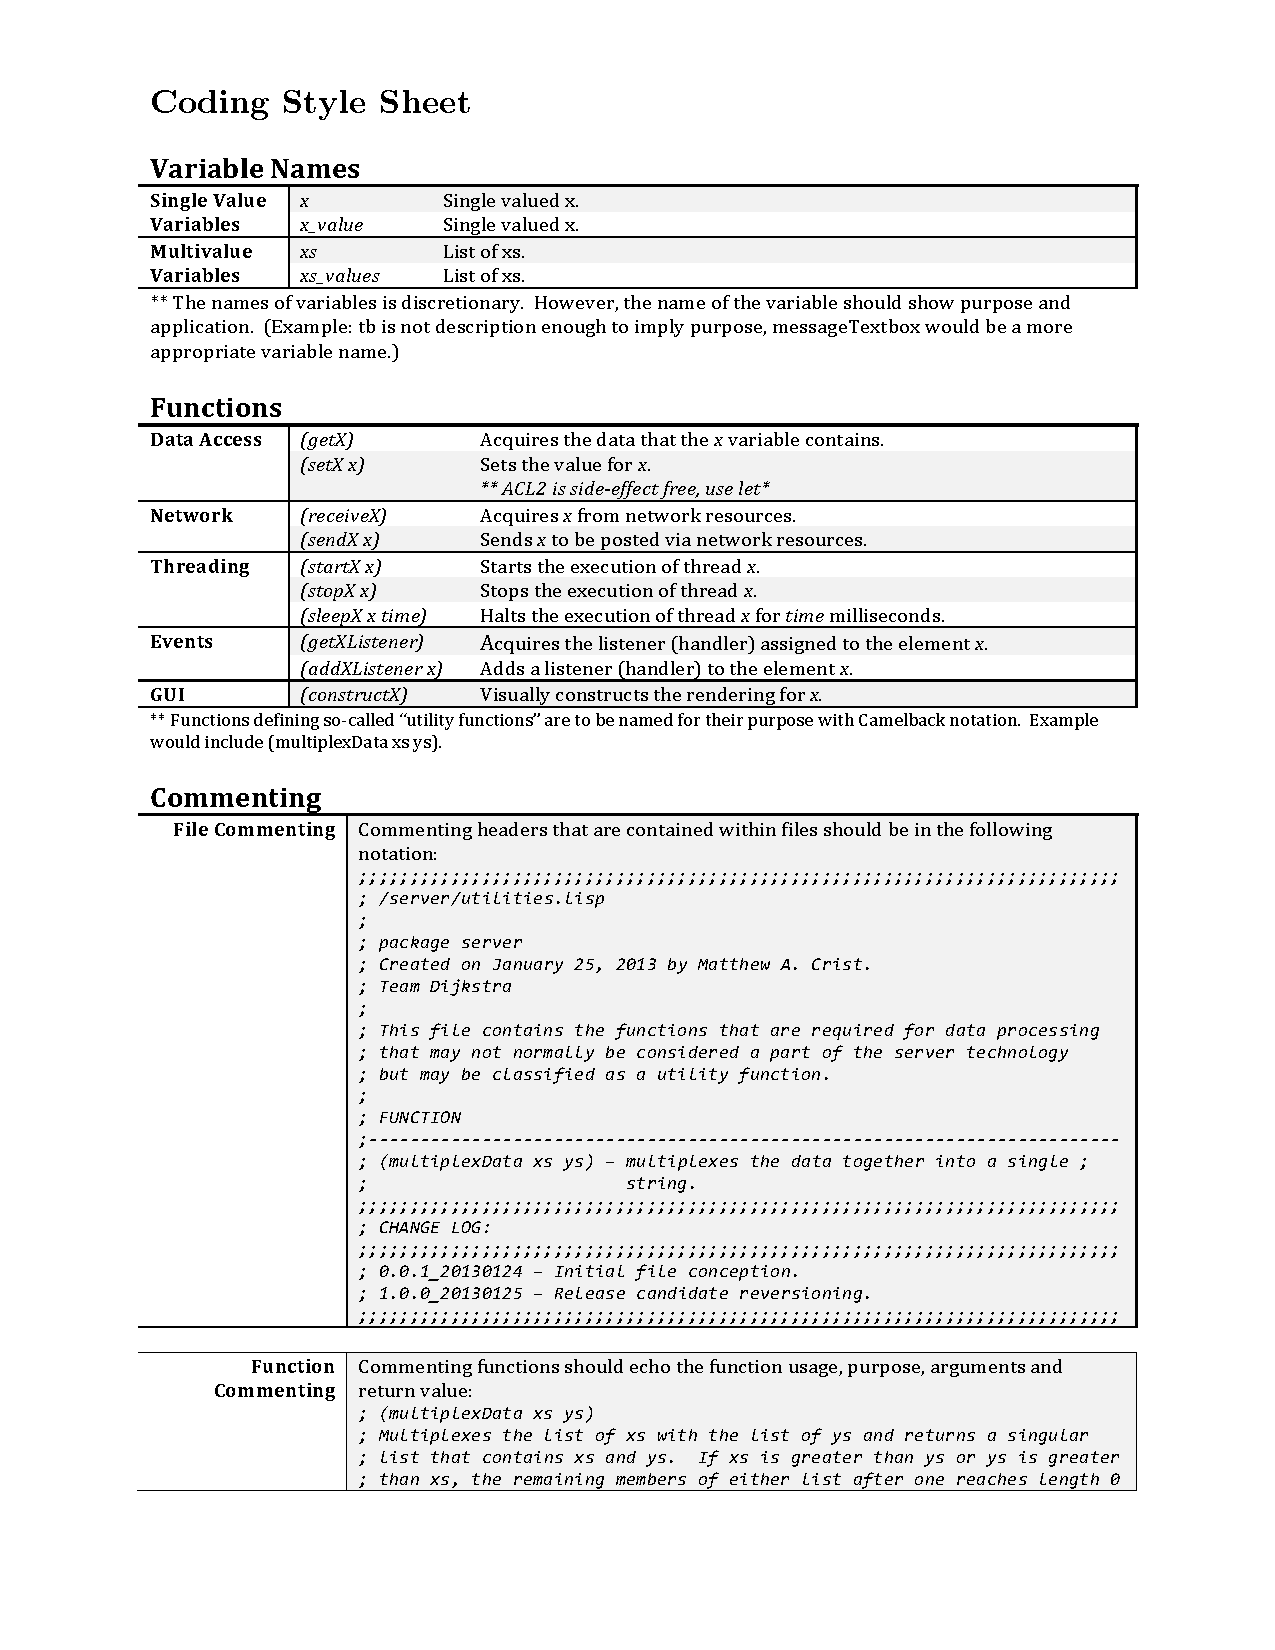
\includepdf[pages=1-2, pagecommand={}, scale=0.95]{CSS}

\newpage
\hypertarget{R} {}
\item[Rationale for Language Choice] \hfill \\ 
This project will make use of standard ACL2. This section will discuss the reasoning for this choice and why we have chosen standard ACL2 over Modular ACL2. \\ \\
The main reason for choosing standard ACL2 is the fact that we can compile the source code rather than have it interpreted through Dracula. Running the code this way will allow the code to be executed much faster and efficiently. This will be beneficial when chat logs become extensive and we have multiple clients running off the server program. Since this program has a large I/O portion, the gains from running the executable code is a compelling reason to use standard ACL2.\\ \\
We plan on using Dr. Racket and Dracula for general development and basic testing. We have chosen this blended environment because of the familiarity with Dr. Racket and the capability of producing executable code from this environment. Another development environment, Proof Pad, was considered, but this environment is primitive and only allows executable code to be ran. We will pass on using this environment due to the unfamiliarity with it and will use Dracula for development and then compiling the code into an executable for running and testing.  \\ \\
The other language choice, Modular ACL2, was not considered since it only runs in Dracula. Modular ACL2 cannot be compiled into an executable and will be slow to execute with our multiple I/O program design. This will become problematic when we decide to use large sets of clients and buffers with the program. Modular ACL2 with Dracula will end up being much slower than running standard ACL2 on the executable code.

\newpage
\hypertarget{P} {}
\item[PROBE Table] \hfill \\ 
The following PROBE Table is to be used for determining an estimate of the number of Lines of Code for a function.  This table was derived from a cumulation of our group members' projects from Software Engineering-I with the addition of the final team project for the semester. \\ \\
There are four basic types of functions that we will implement. The first is a standard non IO function. Most functions will fall into this category. The second is an IO function. These functions will only be those that open and read/modify a file on the system. \\ \\
The final two categories are used to estimate the size of our testing suite. The properties category will be used to classify properties and theorems. Check-Expects are the final category and are used for the check-expect statements in the test suite.\\ \\
The updated PROBE table is as follows:
\begin{table}[htdp]
\begin{center}
\begin{tabular}{lrrrrr}
Function Type & Tiny 7\% & Small 24\% & Medium 38\% & Large 24\% & Huge 7\% \\
\hline
Non IO Functions & 3 & 4 & 6 & 9 & 18 \\
IO Functions & 4 & 5 & 9 & 14 & 16\\
Properties & 3 & 4 & 6 & 8 & 14 \\
Check-Expects & 2 & 3 & 4 & 8 & 14\\
\hline
\end{tabular}
\end{center} 
\end{table}%


\end{description}
\end{document}















































